\documentclass[12pt]{extarticle}
\usepackage[paperwidth=18in,paperheight=8.5in]{geometry}
\usepackage{amsmath}
\usepackage{hyperref}
\usepackage{multirow}
\usepackage{pdfpages}
\usepackage[utf8]{inputenc}
\title{Kaon mixing: chiral and continuum extrapolations}
\author{R Mukherjee}
\date{\today}
\begin{document}
\maketitle
\tableofcontents
\clearpage
\begin{figure}
\centering
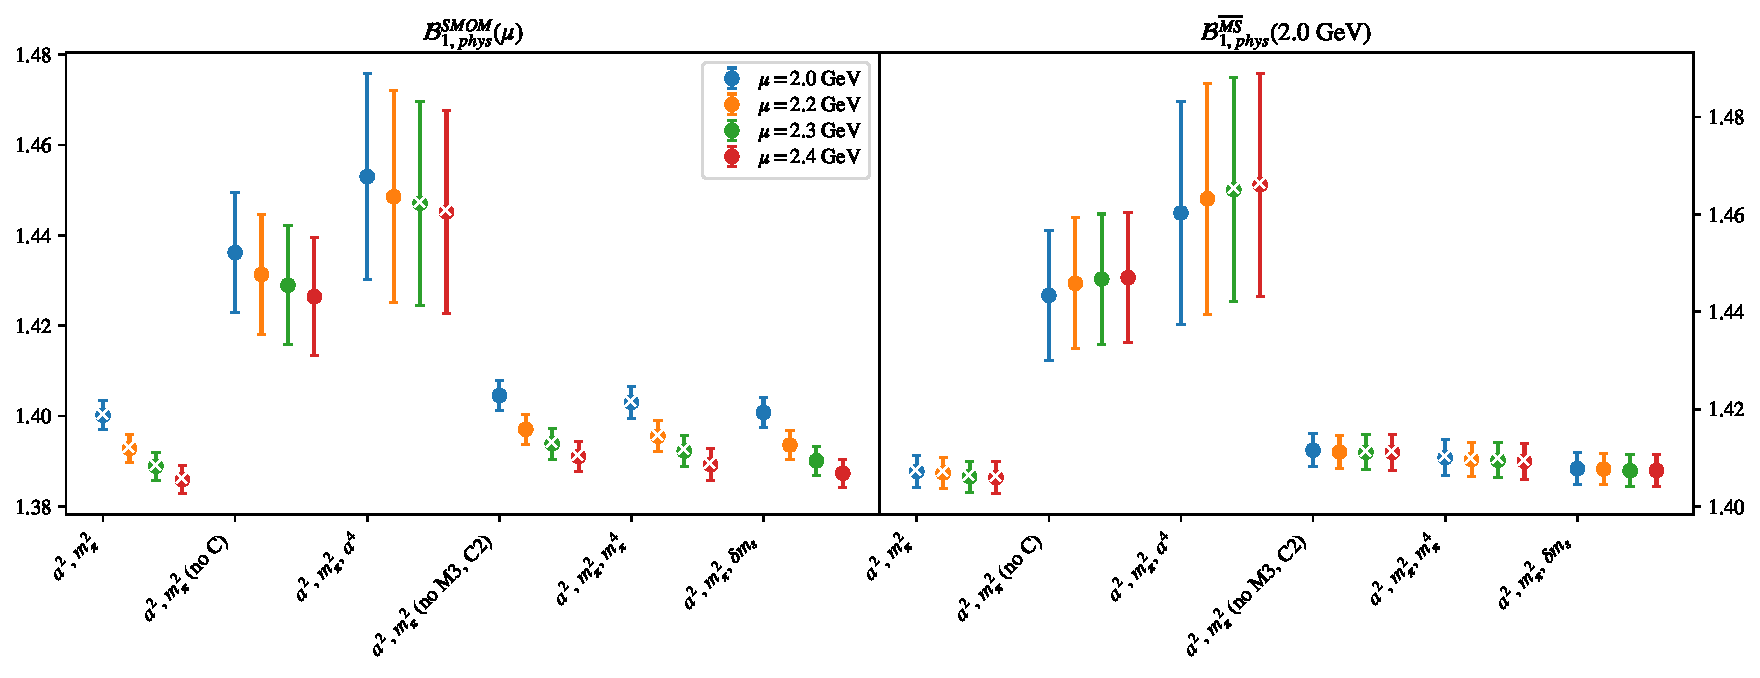
\includegraphics[page=1, width=1.1\textwidth]{VVpAA/NPR/fit_summary_bag.pdf}
\caption{$\mathcal{B}_{1}$\\(left) $\mathcal{B}_{phys}$ in RI/SMOM scheme from fit variations (fits with $p$-value $<0.05$ marked with ``$\times$"). \\(right) $\mathcal{B}_{phys}$ in $\overline{MS}$ computed using $\mathcal{B}^{\overline{MS}} = R^{\overline{MS}\leftarrow SMOM}(2.0)\sigma_{npt}(2.0,\mu) \mathcal{B}^{SMOM}(\mu)$.}
\end{figure}
\clearpage
\begin{figure}
\centering
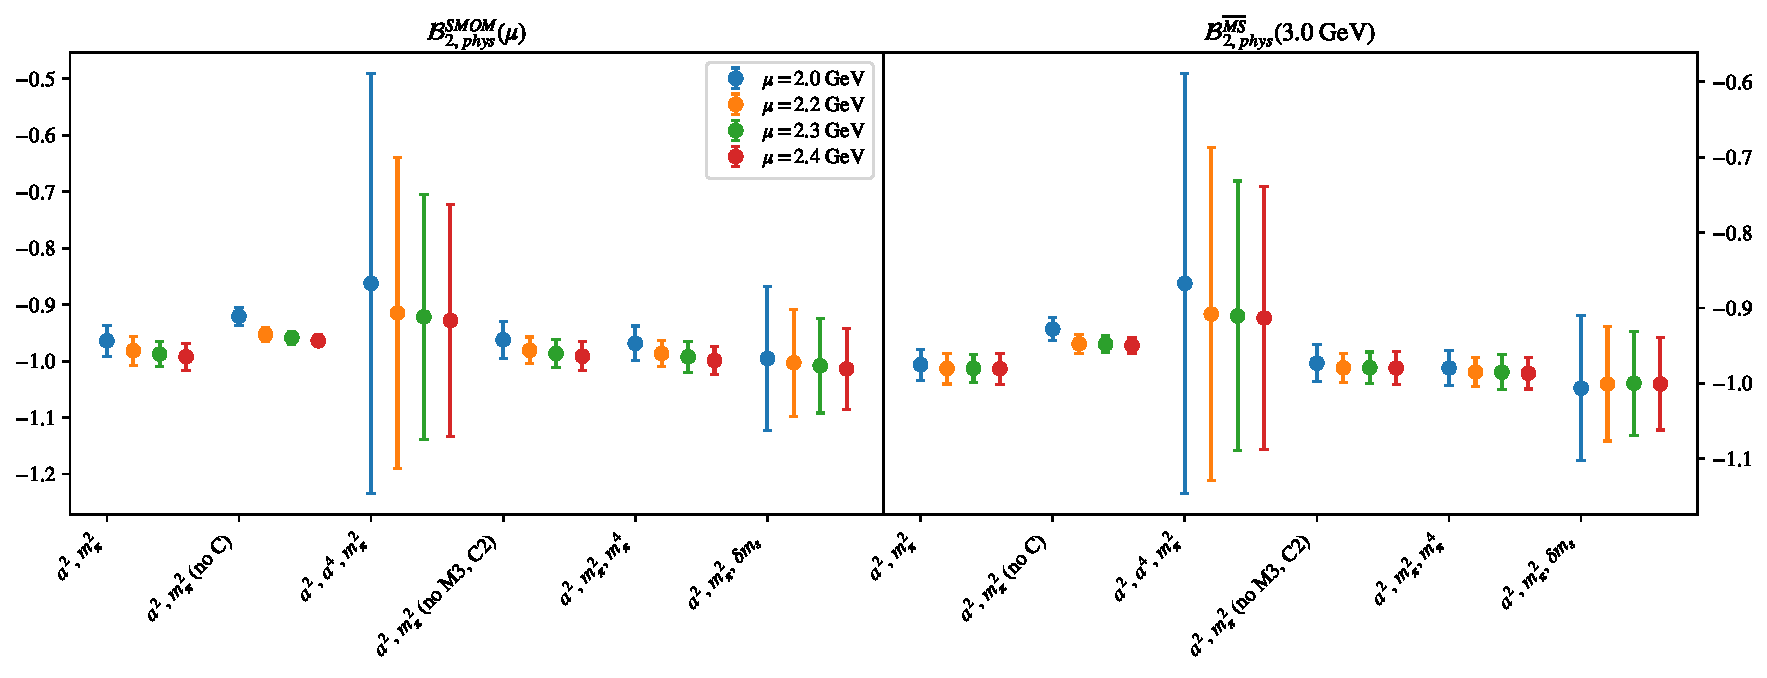
\includegraphics[page=1, width=1.1\textwidth]{VVmAA/NPR/fit_summary_bag.pdf}
\caption{$\mathcal{B}_{2}$\\(left) $\mathcal{B}_{phys}$ in RI/SMOM scheme from fit variations (fits with $p$-value $<0.05$ marked with ``$\times$"). \\(right) $\mathcal{B}_{phys}$ in $\overline{MS}$ computed using $\mathcal{B}^{\overline{MS}} = R^{\overline{MS}\leftarrow SMOM}(3.0)\sigma_{npt}(3.0,\mu) \mathcal{B}^{SMOM}(\mu)$.}
\end{figure}
\clearpage
\begin{figure}
\centering
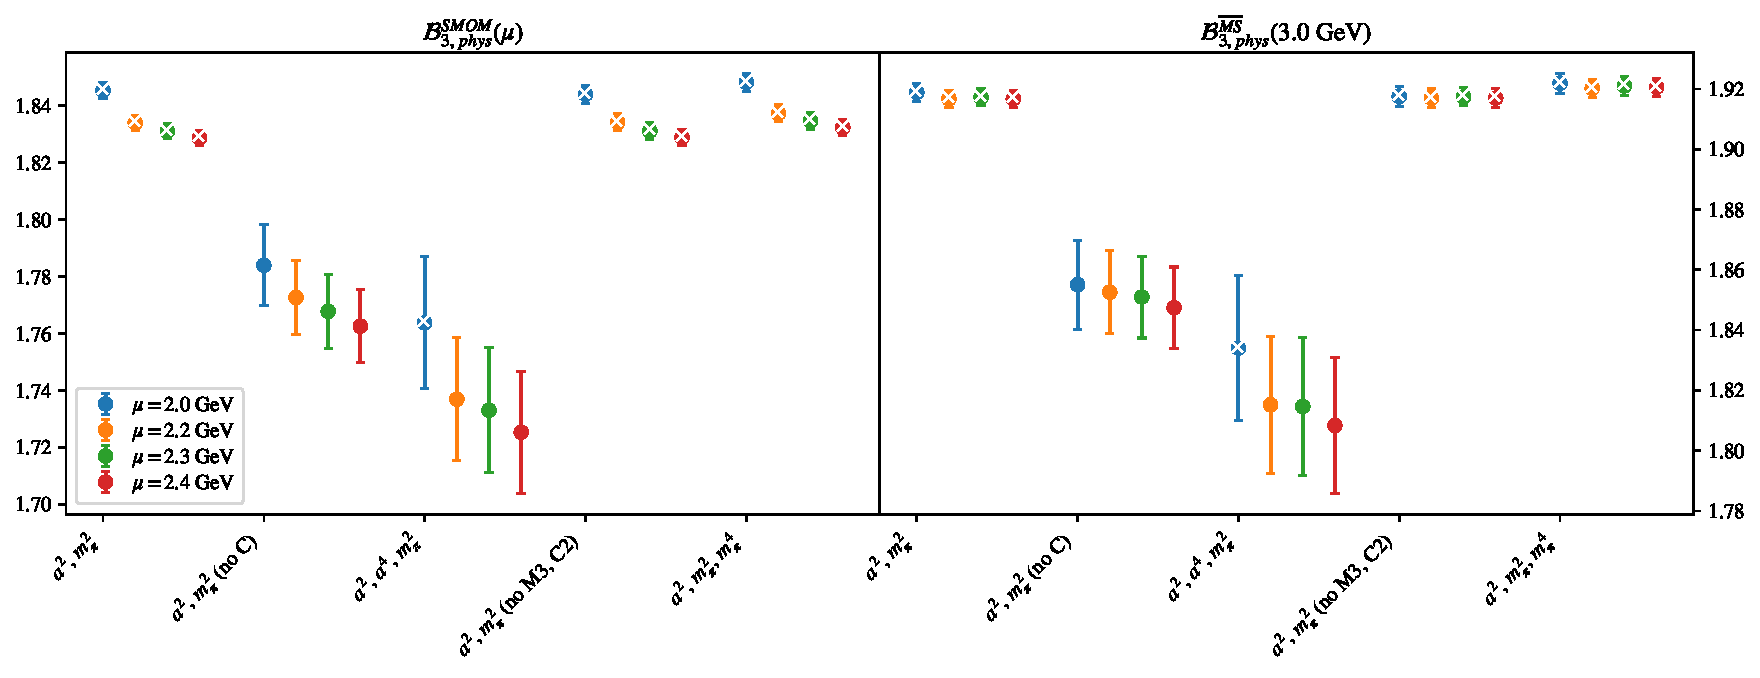
\includegraphics[page=1, width=1.1\textwidth]{SSmPP/NPR/fit_summary_bag.pdf}
\caption{$\mathcal{B}_{3}$\\(left) $\mathcal{B}_{phys}$ in RI/SMOM scheme from fit variations (fits with $p$-value $<0.05$ marked with ``$\times$"). \\(right) $\mathcal{B}_{phys}$ in $\overline{MS}$ computed using $\mathcal{B}^{\overline{MS}} = R^{\overline{MS}\leftarrow SMOM}(3.0)\sigma_{npt}(3.0,\mu) \mathcal{B}^{SMOM}(\mu)$.}
\end{figure}
\clearpage
\begin{figure}
\centering
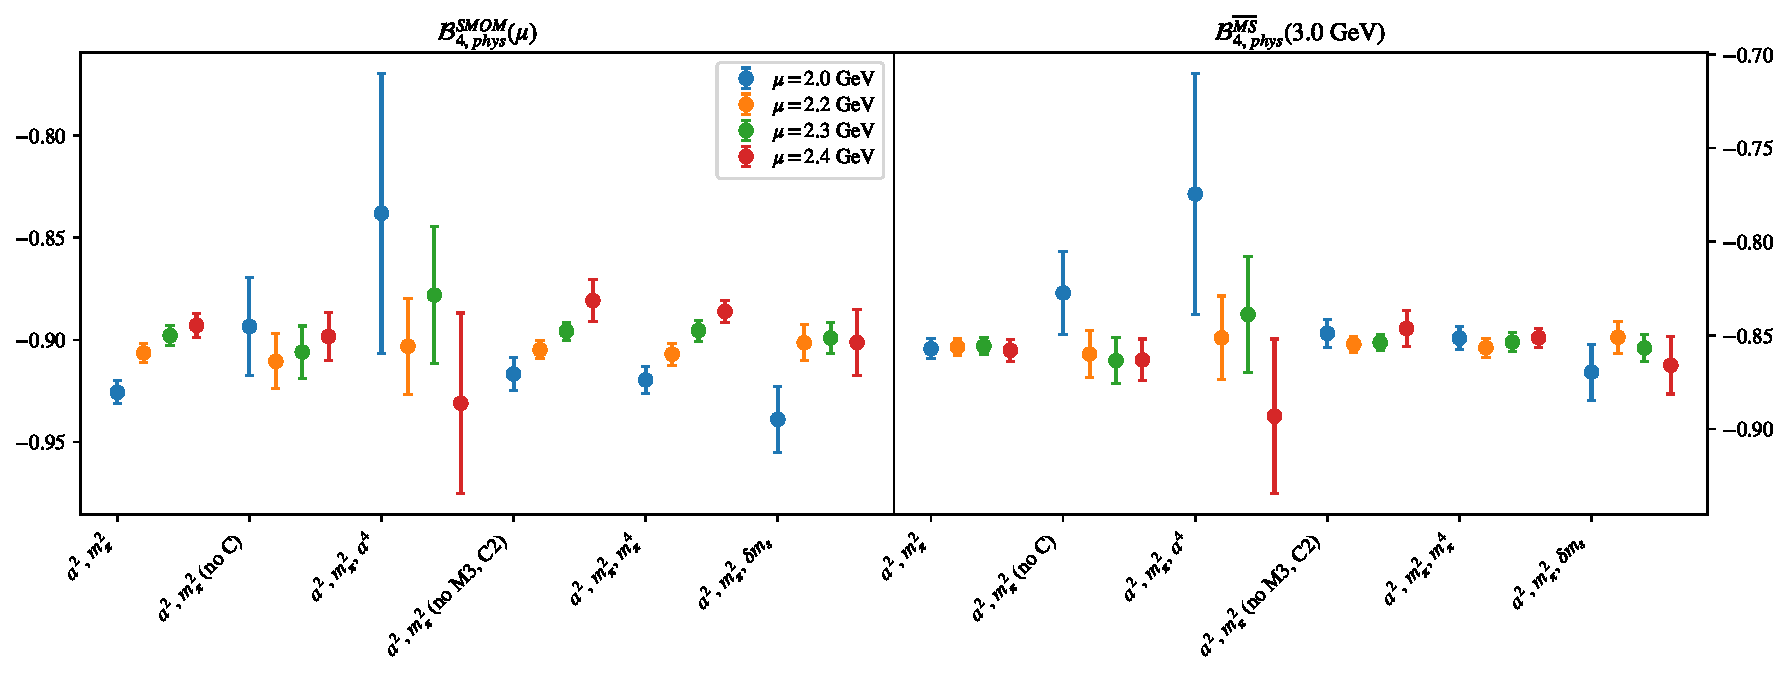
\includegraphics[page=1, width=1.1\textwidth]{SSpPP/NPR/fit_summary_bag.pdf}
\caption{$\mathcal{B}_{4}$\\(left) $\mathcal{B}_{phys}$ in RI/SMOM scheme from fit variations (fits with $p$-value $<0.05$ marked with ``$\times$"). \\(right) $\mathcal{B}_{phys}$ in $\overline{MS}$ computed using $\mathcal{B}^{\overline{MS}} = R^{\overline{MS}\leftarrow SMOM}(3.0)\sigma_{npt}(3.0,\mu) \mathcal{B}^{SMOM}(\mu)$.}
\end{figure}
\clearpage
\begin{figure}
\centering
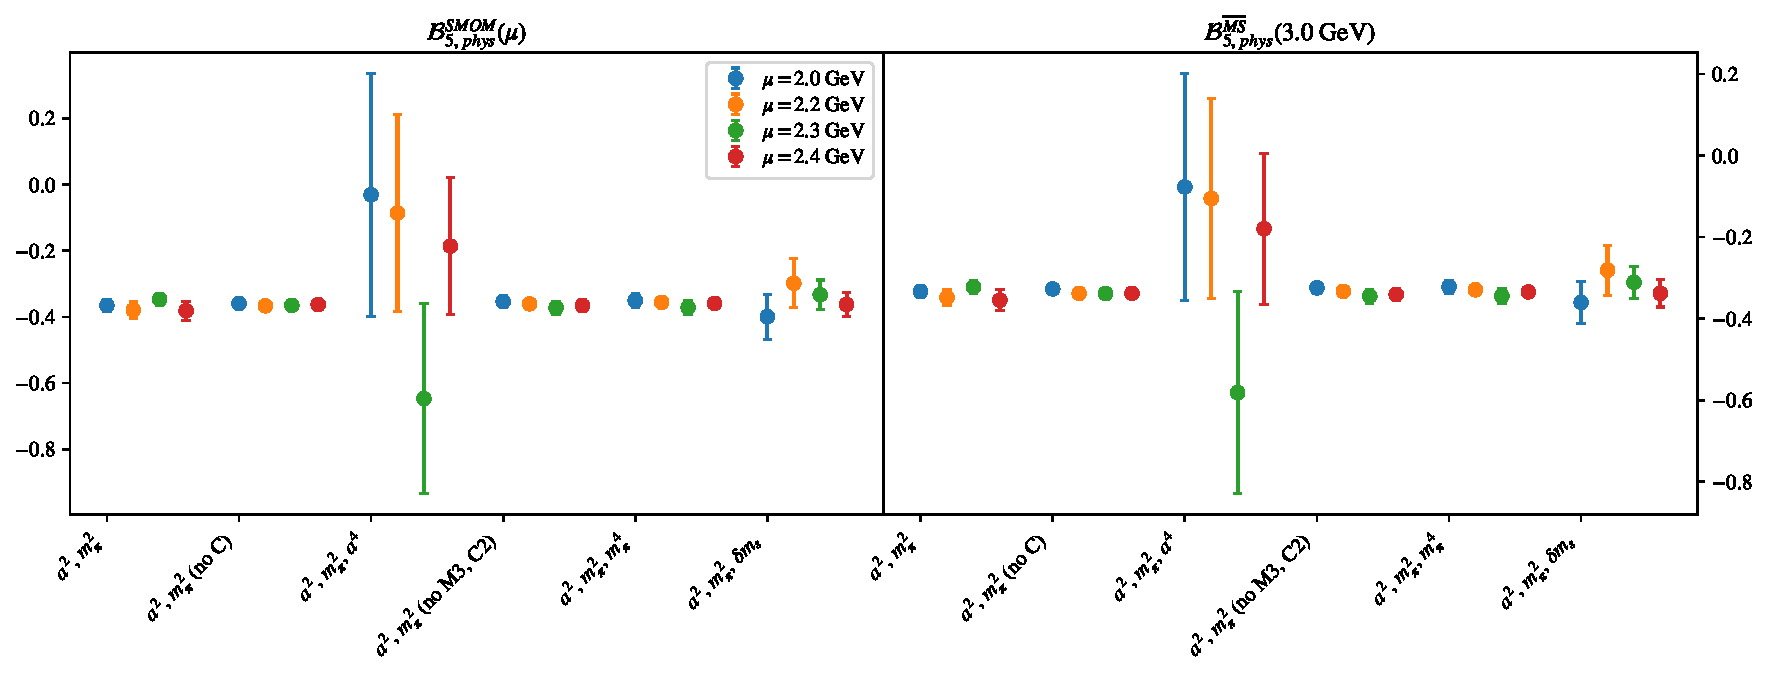
\includegraphics[page=1, width=1.1\textwidth]{TT/NPR/fit_summary_bag.pdf}
\caption{$\mathcal{B}_{5}$\\(left) $\mathcal{B}_{phys}$ in RI/SMOM scheme from fit variations (fits with $p$-value $<0.05$ marked with ``$\times$"). \\(right) $\mathcal{B}_{phys}$ in $\overline{MS}$ computed using $\mathcal{B}^{\overline{MS}} = R^{\overline{MS}\leftarrow SMOM}(3.0)\sigma_{npt}(3.0,\mu) \mathcal{B}^{SMOM}(\mu)$.}
\end{figure}
\clearpage
\section{$\mathcal{B}_1$}
\begin{table}[h!]
\begin{center}
\begin{tabular}{|c|c|c|c|c|c|c|}
\hline
$\mu$ (GeV) & $a^2$, $m_\pi^2$& $a^2$, $m_\pi^2$ (no C)& $a^2$, $m_\pi^2$, $a^4$& $a^2$, $m_\pi^2$ (no M3, C2)& $a^2$, $m_\pi^2$, $m_\pi^4$& $a^2$, $m_\pi^2$, $\delta m_s$\\
\hline
2.0& \hyperlink{VVpAA/NPR/a2m2_20.pdf.1}{\textbf{1.4018(27)}: 2.317 (0.041)} & \hyperlink{VVpAA/NPR/a2m2noC_20.pdf.1}{\textbf{1.417(12)}: 0.876 (0.417)} & \hyperlink{VVpAA/NPR/a2a4m2_20.pdf.1}{\textbf{1.421(21)}: 2.793 (0.025)} & \hyperlink{VVpAA/NPR/a2m2mcut_20.pdf.1}{\textbf{1.4064(36)}: 0.219 (0.883)} & \hyperlink{VVpAA/NPR/a2m2m4_20.pdf.1}{\textbf{1.4066(36)}: 0.977 (0.419)} & \hyperlink{VVpAA/NPR/a2m2delm_20.pdf.1}{\textbf{1.3992(33)}: 2.43 (0.045)}\\
2.2& \hyperlink{VVpAA/NPR/a2m2_22.pdf.1}{\textbf{1.3947(27)}: 2.657 (0.021)} & \hyperlink{VVpAA/NPR/a2m2noC_22.pdf.1}{\textbf{1.412(12)}: 1.018 (0.361)} & \hyperlink{VVpAA/NPR/a2a4m2_22.pdf.1}{\textbf{1.417(21)}: 3.136 (0.014)} & \hyperlink{VVpAA/NPR/a2m2mcut_22.pdf.1}{\textbf{1.3995(36)}: 0.359 (0.782)} & \hyperlink{VVpAA/NPR/a2m2m4_22.pdf.1}{\textbf{1.3995(36)}: 1.227 (0.297)} & \hyperlink{VVpAA/NPR/a2m2delm_22.pdf.1}{\textbf{1.3919(32)}: 2.651 (0.031)}\\
2.3& \hyperlink{VVpAA/NPR/a2m2_23.pdf.1}{\textbf{1.3912(27)}: 2.892 (0.013)} & \hyperlink{VVpAA/NPR/a2m2noC_23.pdf.1}{\textbf{1.410(12)}: 1.097 (0.334)} & \hyperlink{VVpAA/NPR/a2a4m2_23.pdf.1}{\textbf{1.415(21)}: 3.386 (0.009)} & \hyperlink{VVpAA/NPR/a2m2mcut_23.pdf.1}{\textbf{1.3962(36)}: 0.452 (0.716)} & \hyperlink{VVpAA/NPR/a2m2m4_23.pdf.1}{\textbf{1.3962(36)}: 1.407 (0.229)} & \hyperlink{VVpAA/NPR/a2m2delm_23.pdf.1}{\textbf{1.3882(31)}: 2.818 (0.024)}\\
2.4& \hyperlink{VVpAA/NPR/a2m2_24.pdf.1}{\textbf{1.3883(26)}: 2.991 (0.011)} & \hyperlink{VVpAA/NPR/a2m2noC_24.pdf.1}{\textbf{1.408(12)}: 1.148 (0.317)} & \hyperlink{VVpAA/NPR/a2a4m2_24.pdf.1}{\textbf{1.413(21)}: 3.498 (0.007)} & \hyperlink{VVpAA/NPR/a2m2mcut_24.pdf.1}{\textbf{1.3934(37)}: 0.474 (0.7)} & \hyperlink{VVpAA/NPR/a2m2m4_24.pdf.1}{\textbf{1.3934(36)}: 1.461 (0.211)} & \hyperlink{VVpAA/NPR/a2m2delm_24.pdf.1}{\textbf{1.3852(31)}: 2.9 (0.021)}\\
\hline
\end{tabular}
\caption{Physical point value from chiral and continuum extrapolation at renormalisation scale $\mu$. Entries are \textbf{value(error)}: $\chi^2/\text{DOF}$ ($p$-value).}
\end{center}
\end{table}
\begin{table}[h!]
\begin{center}
\begin{tabular}{|c c|c|c|c|c|c|c|}
\hline
$\mu$ (GeV) &  & $a^2$, $m_\pi^2$& $a^2$, $m_\pi^2$ (no C)& $a^2$, $m_\pi^2$, $a^4$& $a^2$, $m_\pi^2$ (no M3, C2)& $a^2$, $m_\pi^2$, $m_\pi^4$& $a^2$, $m_\pi^2$, $\delta m_s$\\
\hline
\multirow{3}{0.5in}{2.0} & $\alpha$ & 0.1035(98)& 0.042(53)& -0.024& 0.092(12)& 0.092(12)& 0.109(11)\\
 & $\beta$ & 0.00290(16)& 0.00246(34)& 0.00293(16)& 0.00222(35)& 0.001& 0.00302(17)\\
 & $\gamma$ &  &  & 0.25(28)&  & 0.000181(89)& -0.003(24)\\
\hline
\multirow{3}{0.5in}{2.2} & $\alpha$ & 0.1067(94)& 0.037(52)& -0.045& 0.095(12)& 0.095(12)& 0.113(10)\\
 & $\beta$ & 0.00286(15)& 0.00243(36)& 0.00290(16)& 0.00217(37)& 0.001& 0.00300(17)\\
 & $\gamma$ &  &  & 0.30(28)&  & 0.000182(92)& -0.004(24)\\
\hline
\multirow{3}{0.5in}{2.3} & $\alpha$ & 0.1088(96)& 0.032(51)& -0.054& 0.096(12)& 0.097(12)& 0.116(10)\\
 & $\beta$ & 0.00285(16)& 0.00237(35)& 0.00289(16)& 0.00213(37)& 0.001& 0.00300(17)\\
 & $\gamma$ &  &  & 0.32(27)&  & 0.000189(91)& -0.004(24)\\
\hline
\multirow{3}{0.5in}{2.4} & $\alpha$ & 0.1097(96)& 0.032(51)& -0.055& 0.097(12)& 0.097(12)& 0.117(10)\\
 & $\beta$ & 0.00285(16)& 0.00237(36)& 0.00289(16)& 0.00213(37)& 0.001& 0.00300(17)\\
 & $\gamma$ &  &  & 0.32(27)&  & 0.000191(91)& -0.004(23)\\
\hline
\end{tabular}
\caption{Fit values of coefficients in $Q = Q_{phys} + \mathbf{\alpha} a^2 + \mathbf{\beta}\left(\frac{m_\pi^2}{f_\pi^2}-\frac{m_{\pi,PDG}^2}{f_\pi^2}\right) + \gamma(\ldots)$}
\end{center}
\end{table}
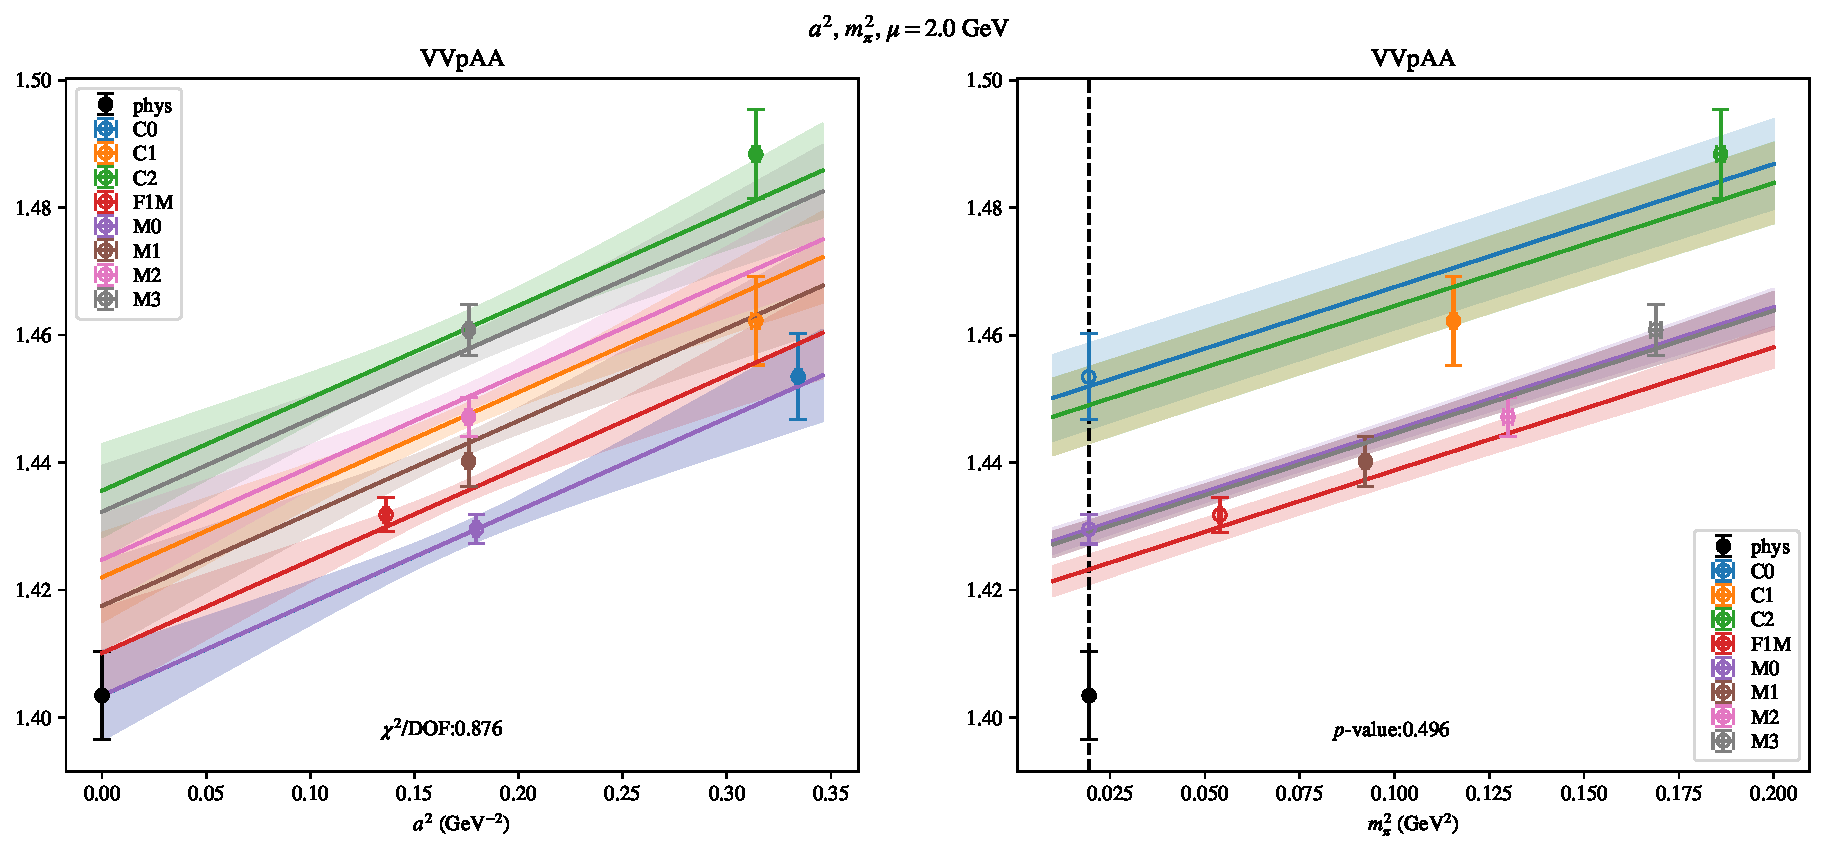
\includepdf[link, pages=-]{VVpAA/NPR/a2m2_20.pdf}
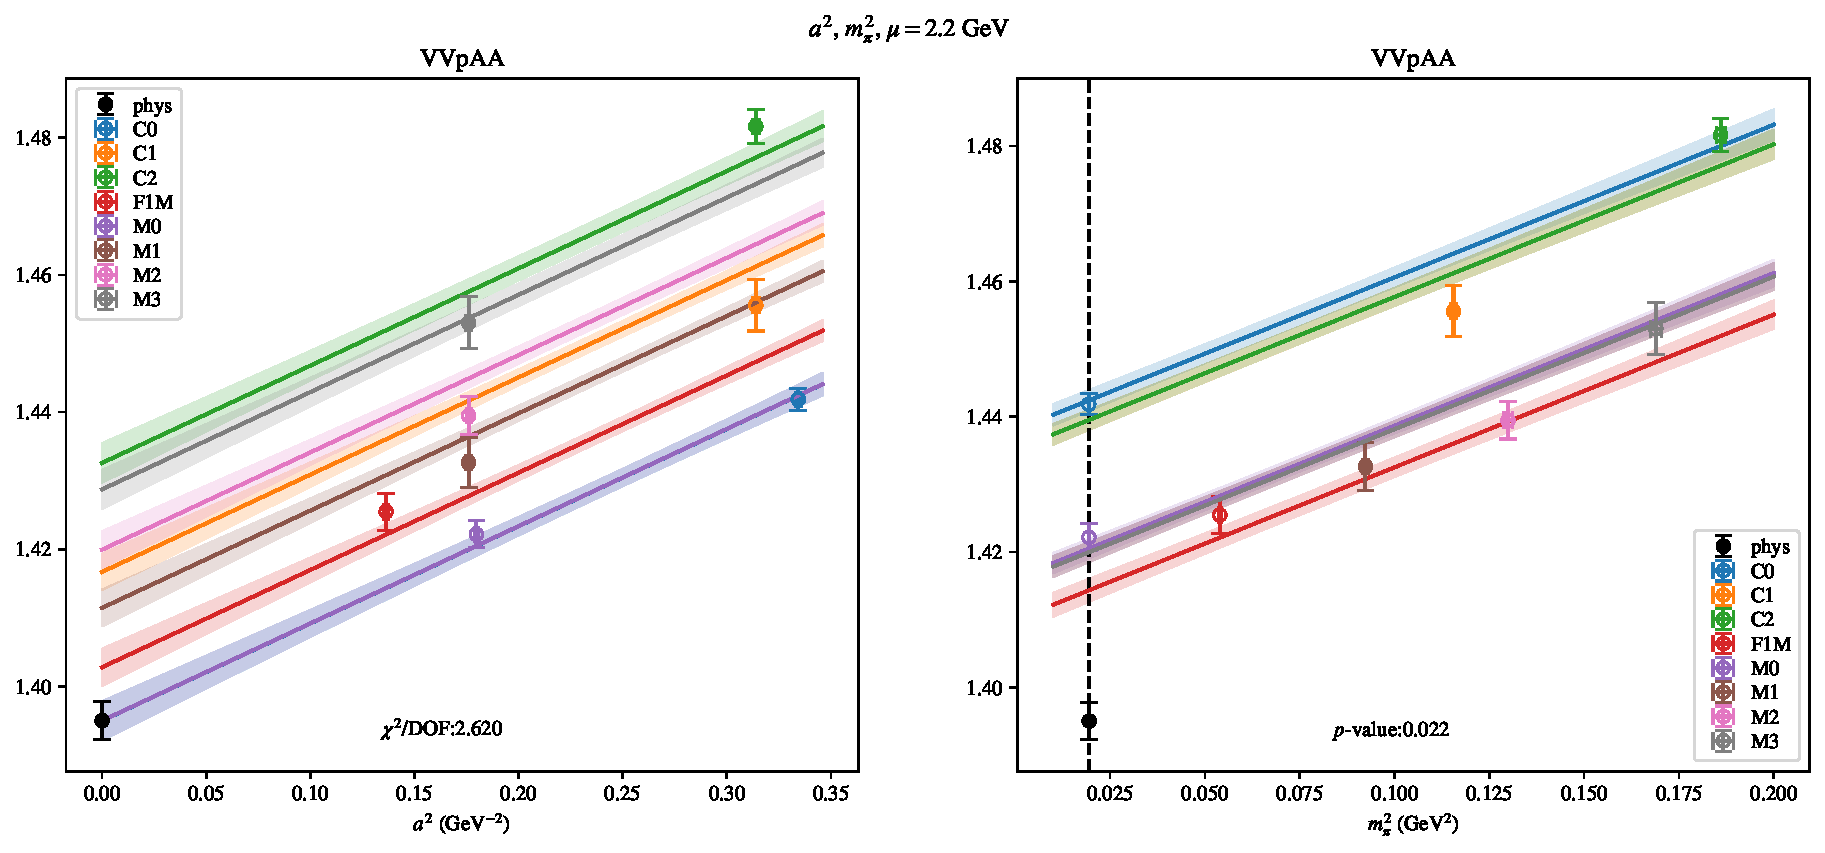
\includepdf[link, pages=-]{VVpAA/NPR/a2m2_22.pdf}
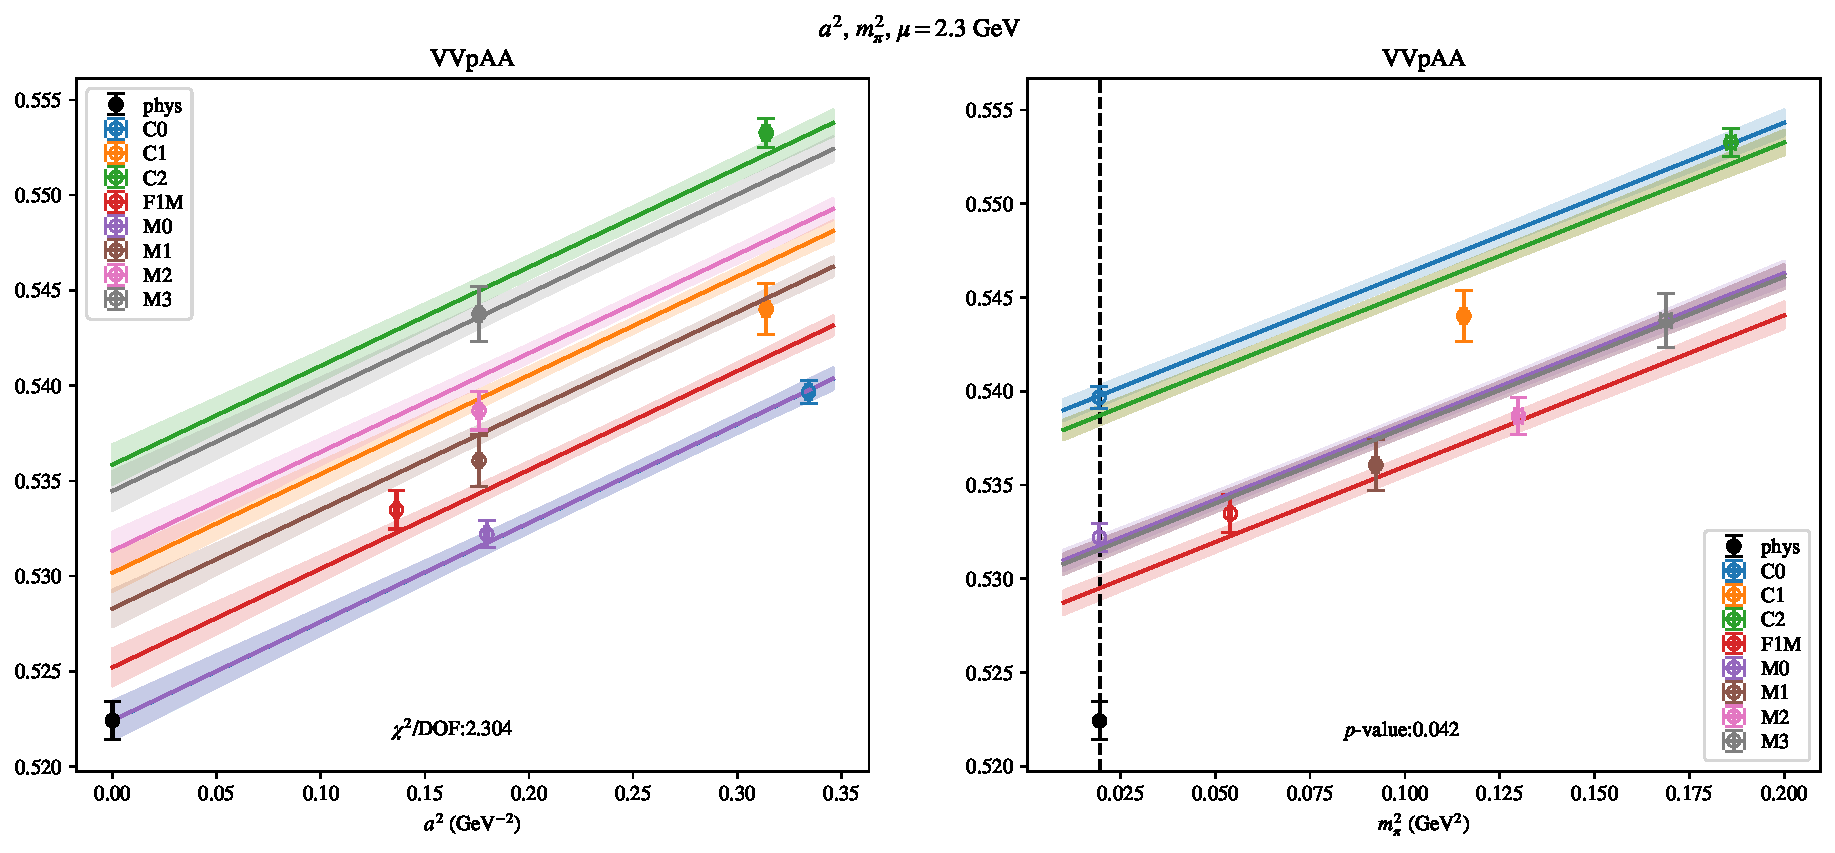
\includepdf[link, pages=-]{VVpAA/NPR/a2m2_23.pdf}
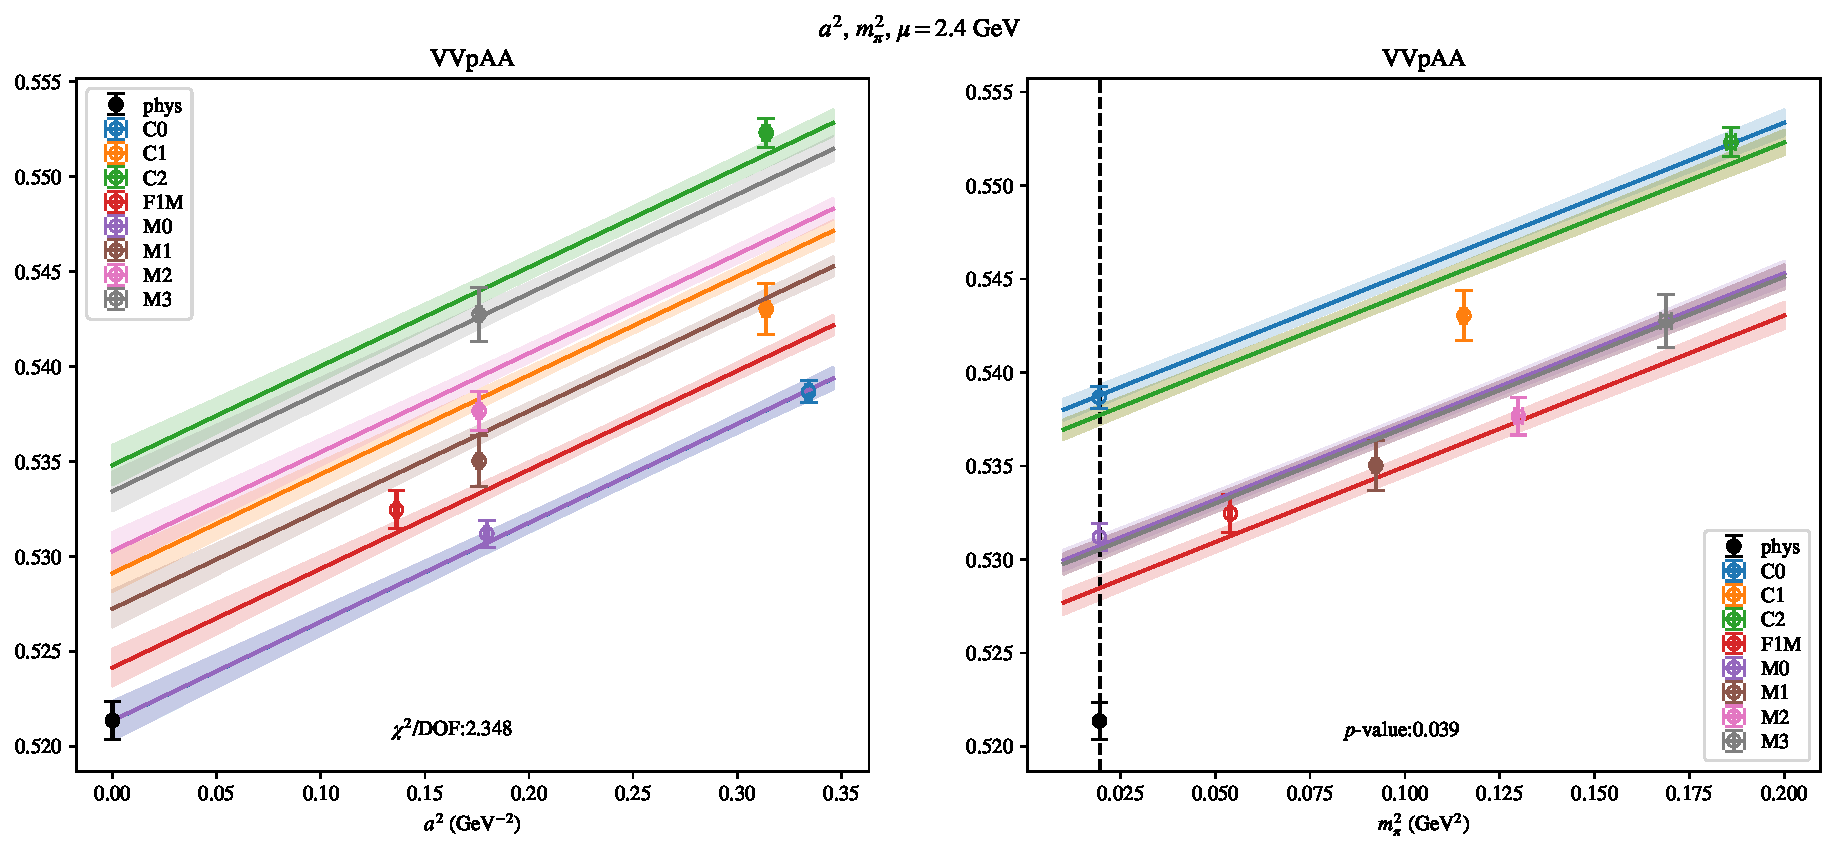
\includepdf[link, pages=-]{VVpAA/NPR/a2m2_24.pdf}
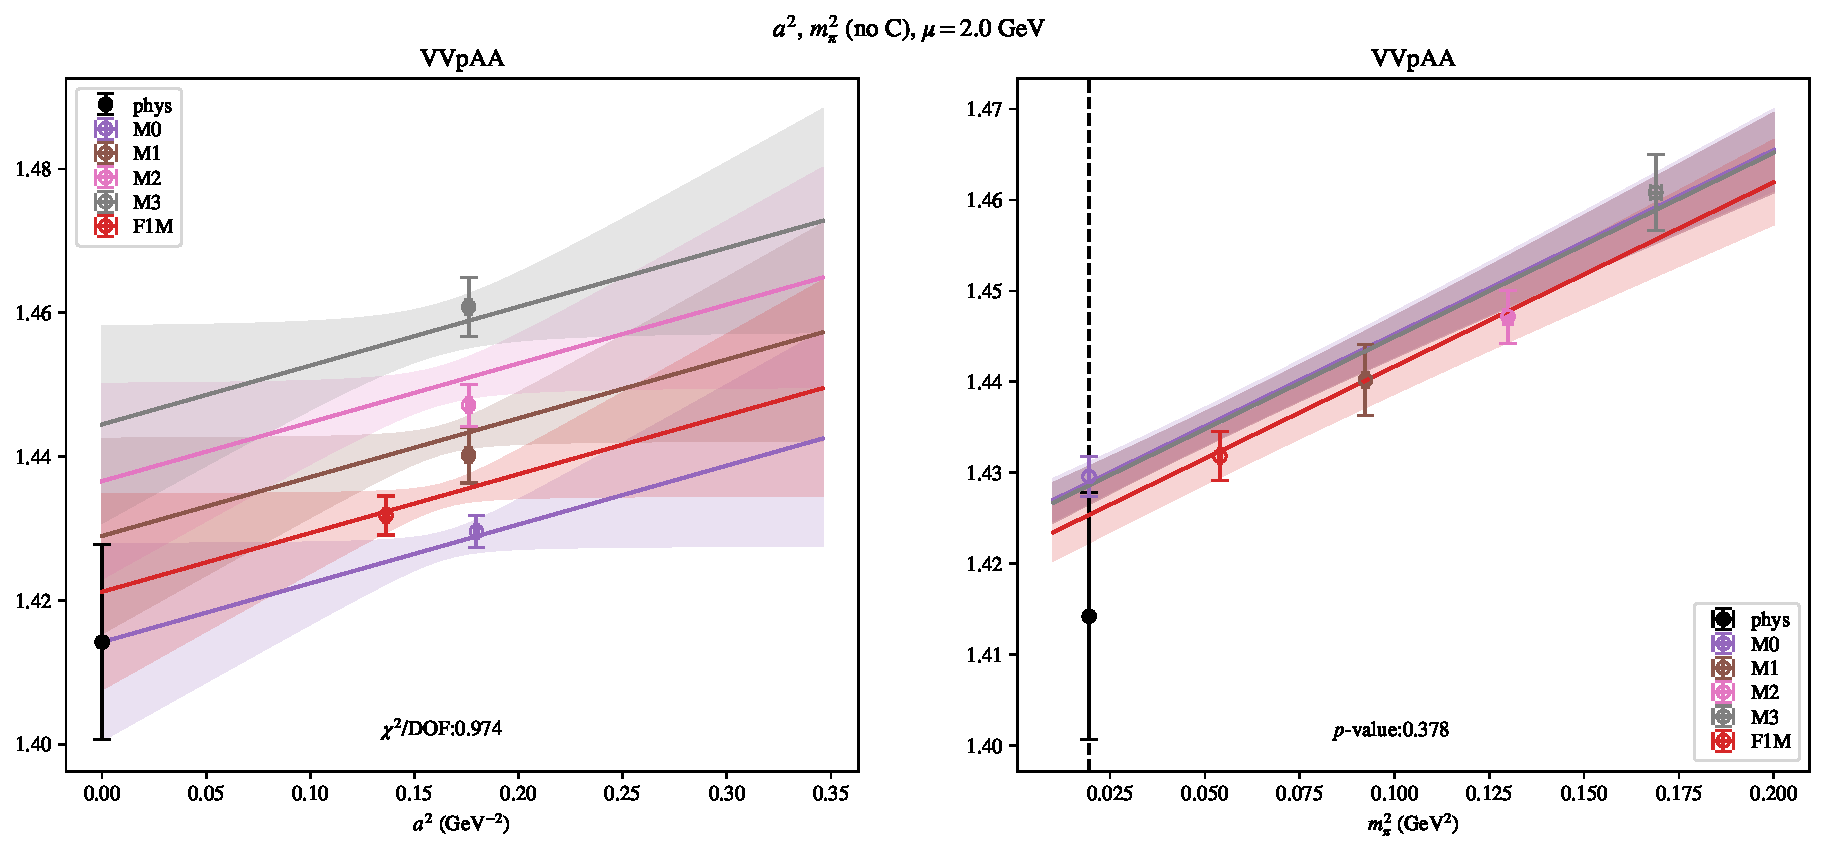
\includepdf[link, pages=-]{VVpAA/NPR/a2m2noC_20.pdf}
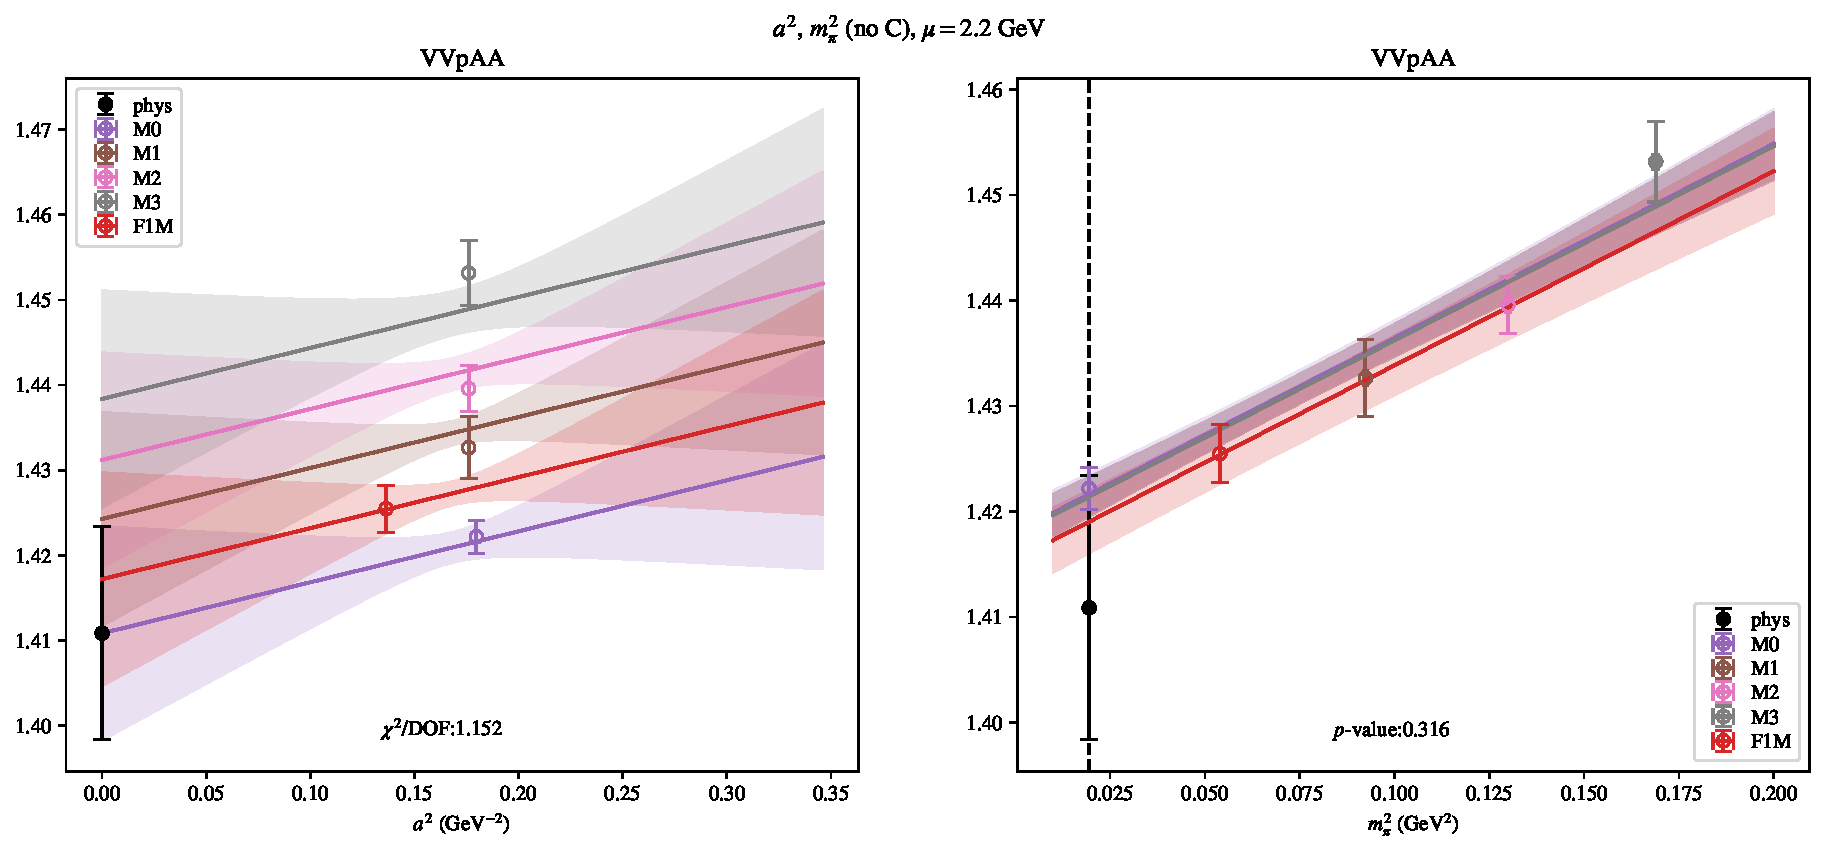
\includepdf[link, pages=-]{VVpAA/NPR/a2m2noC_22.pdf}
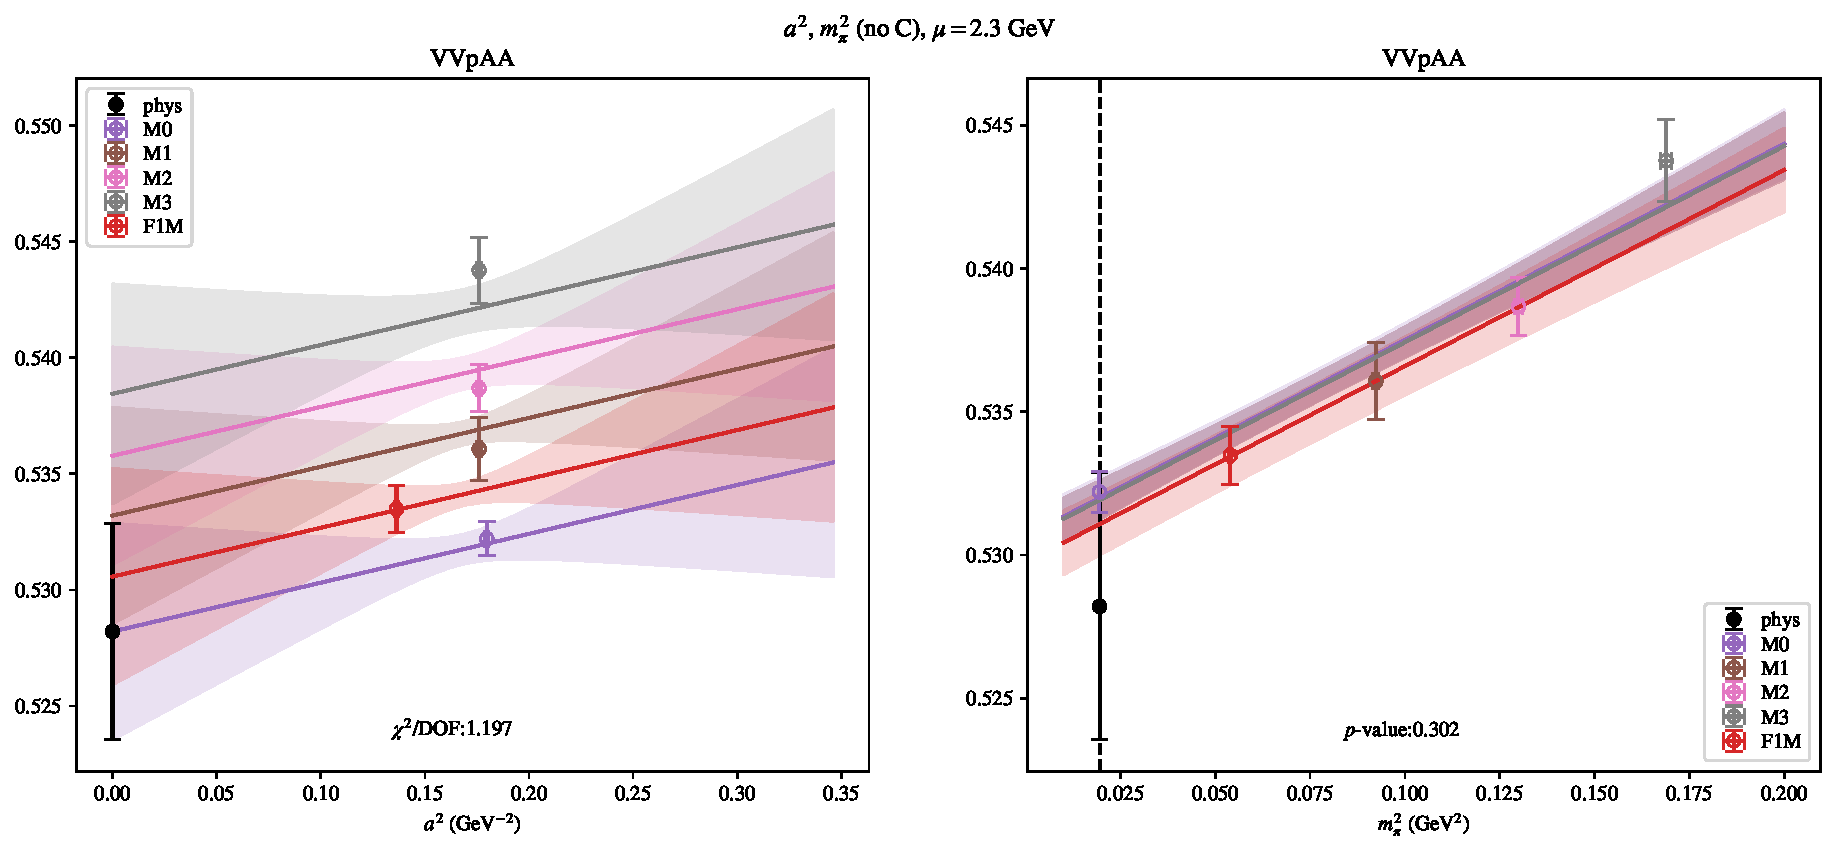
\includepdf[link, pages=-]{VVpAA/NPR/a2m2noC_23.pdf}
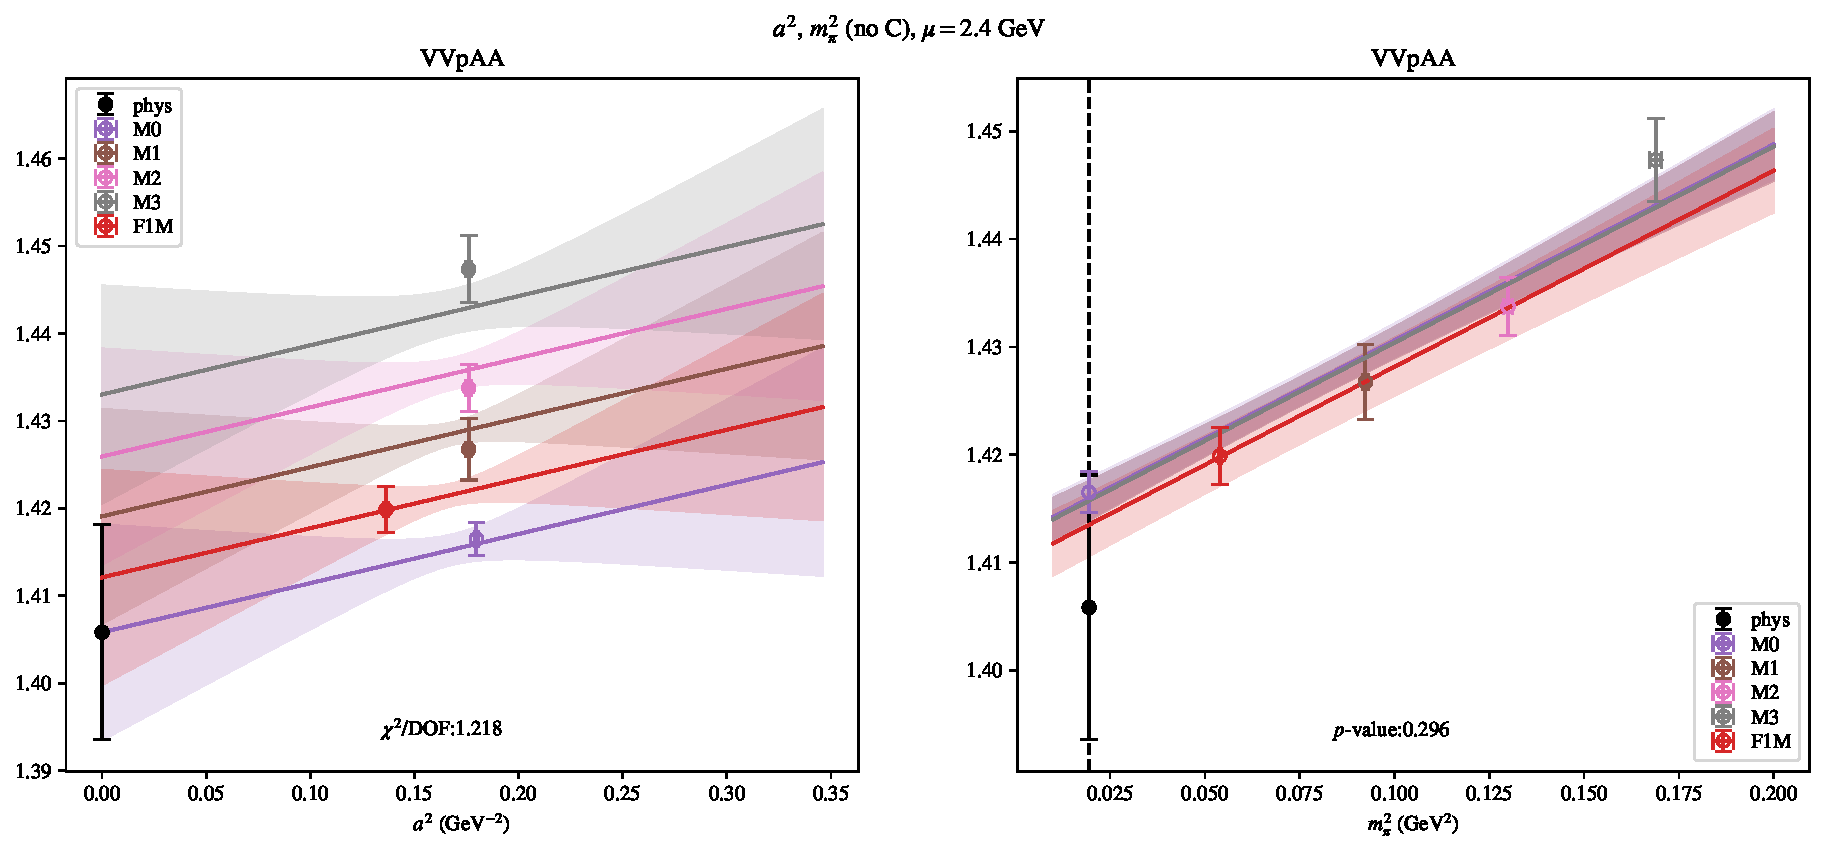
\includepdf[link, pages=-]{VVpAA/NPR/a2m2noC_24.pdf}
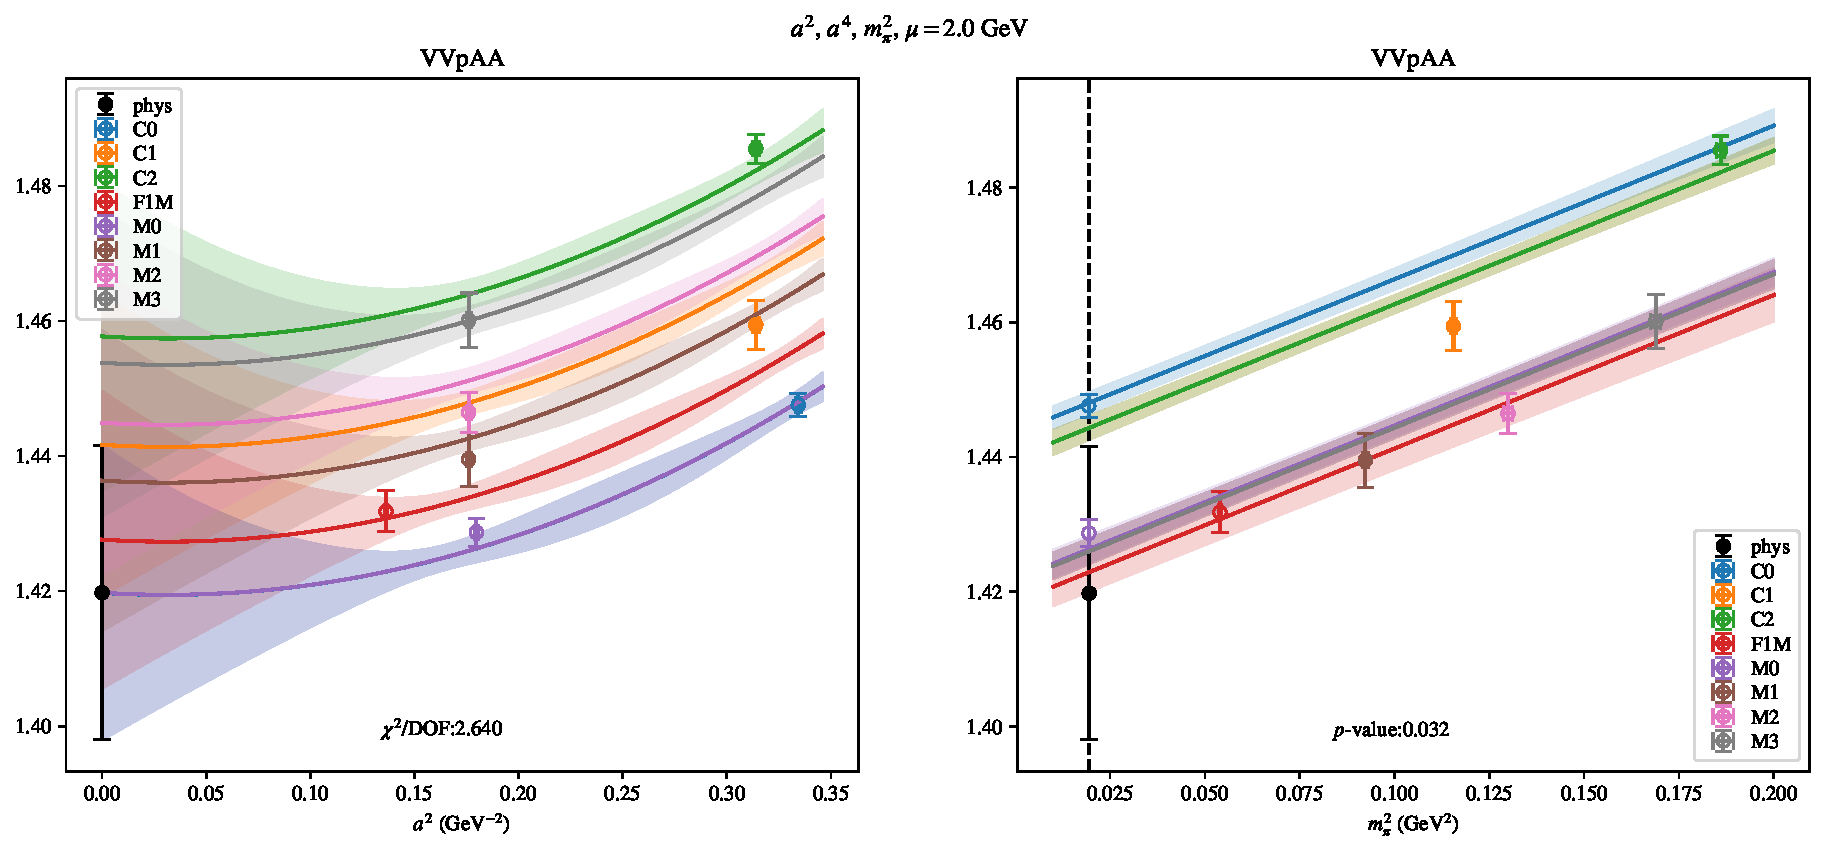
\includepdf[link, pages=-]{VVpAA/NPR/a2a4m2_20.pdf}
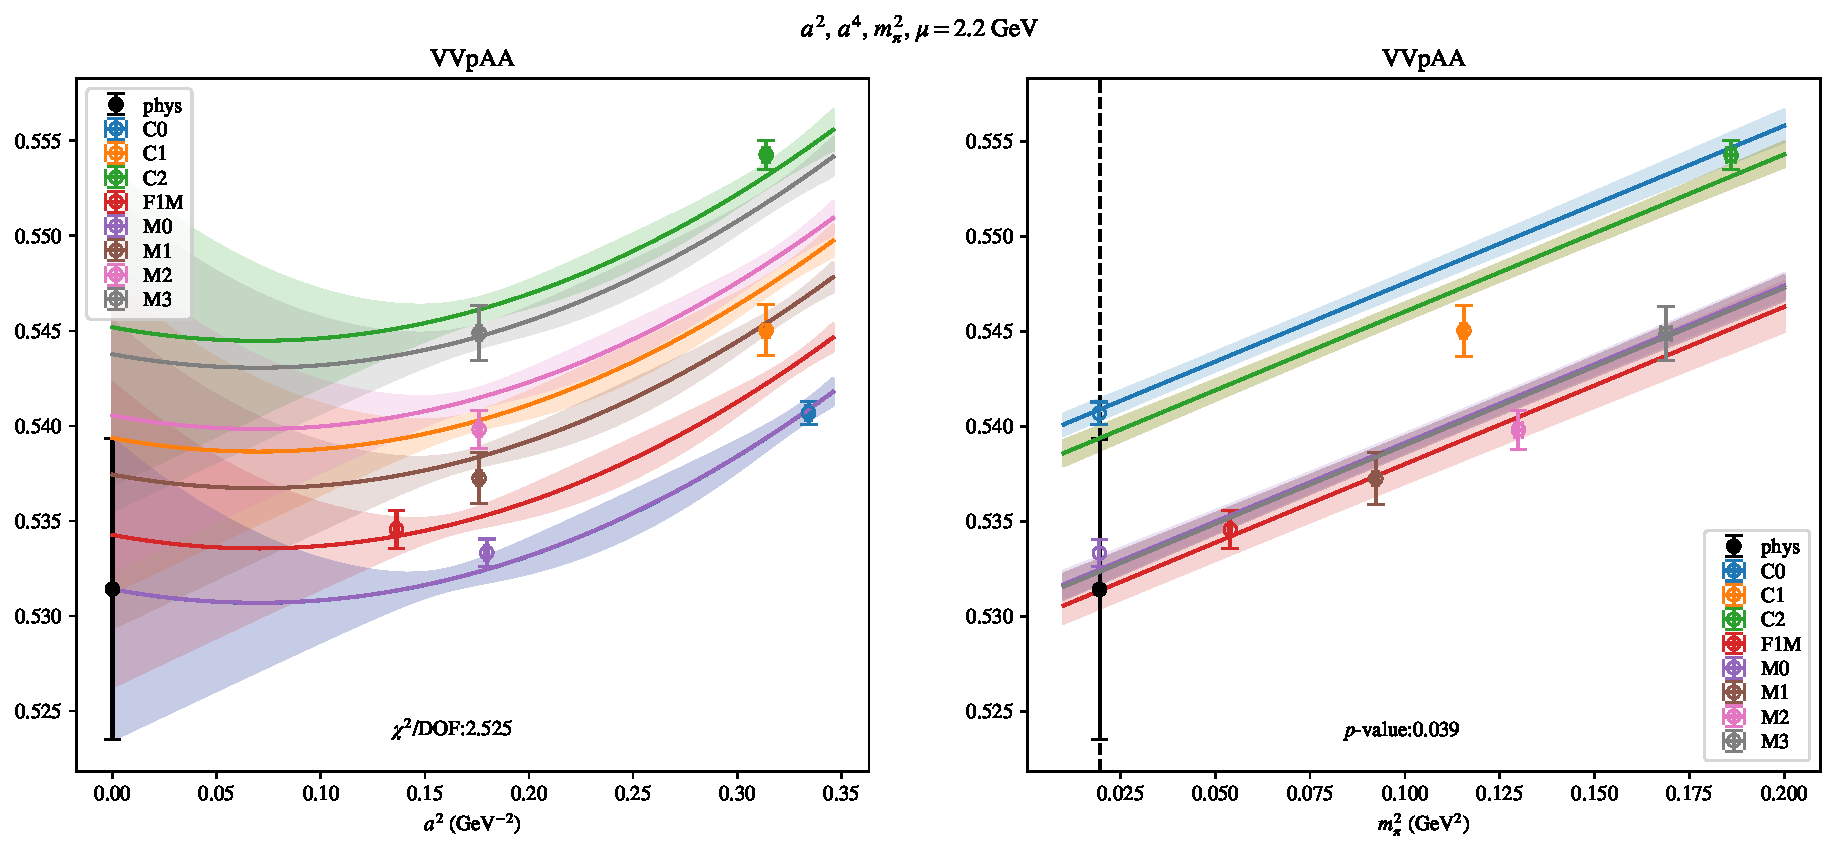
\includepdf[link, pages=-]{VVpAA/NPR/a2a4m2_22.pdf}
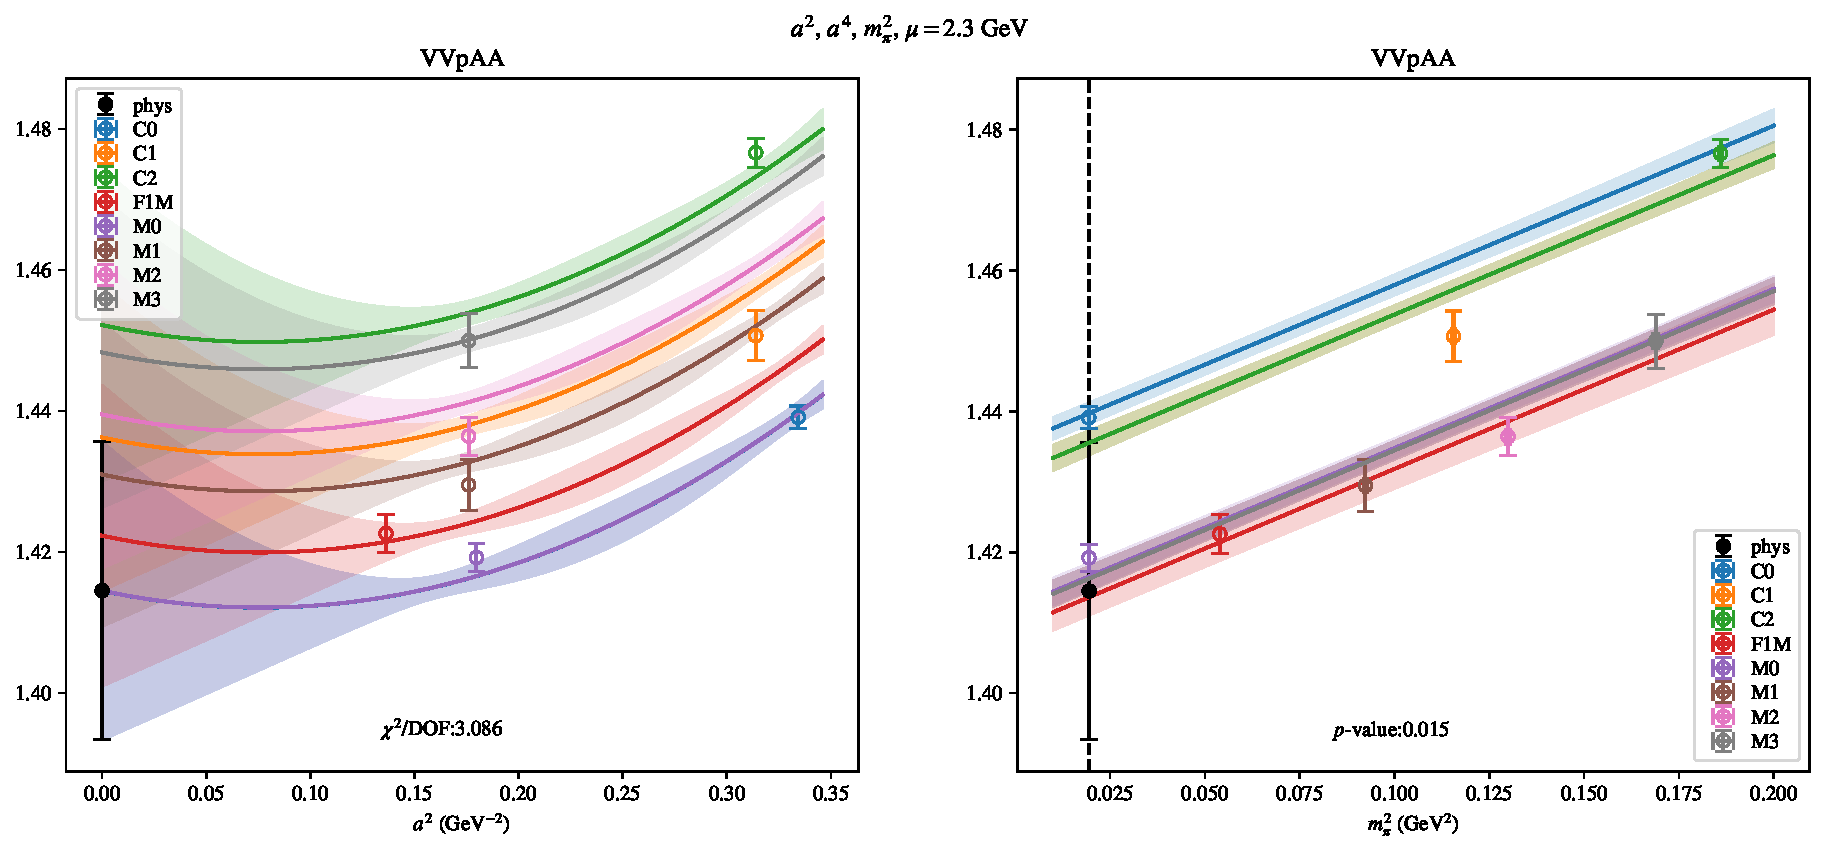
\includepdf[link, pages=-]{VVpAA/NPR/a2a4m2_23.pdf}
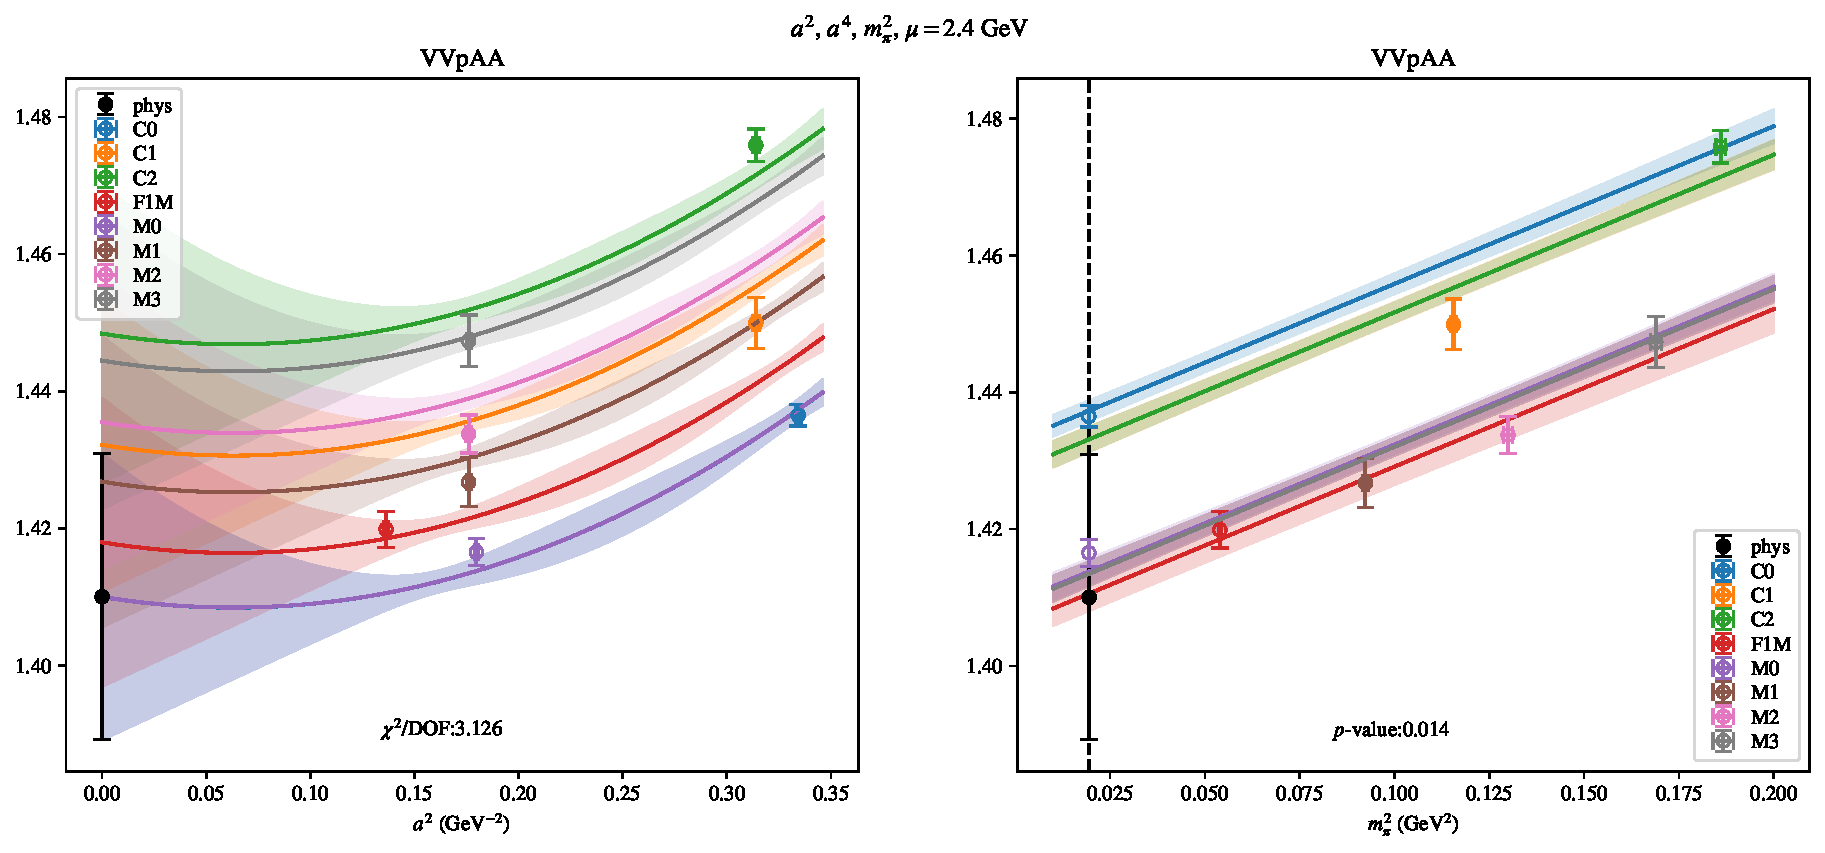
\includepdf[link, pages=-]{VVpAA/NPR/a2a4m2_24.pdf}
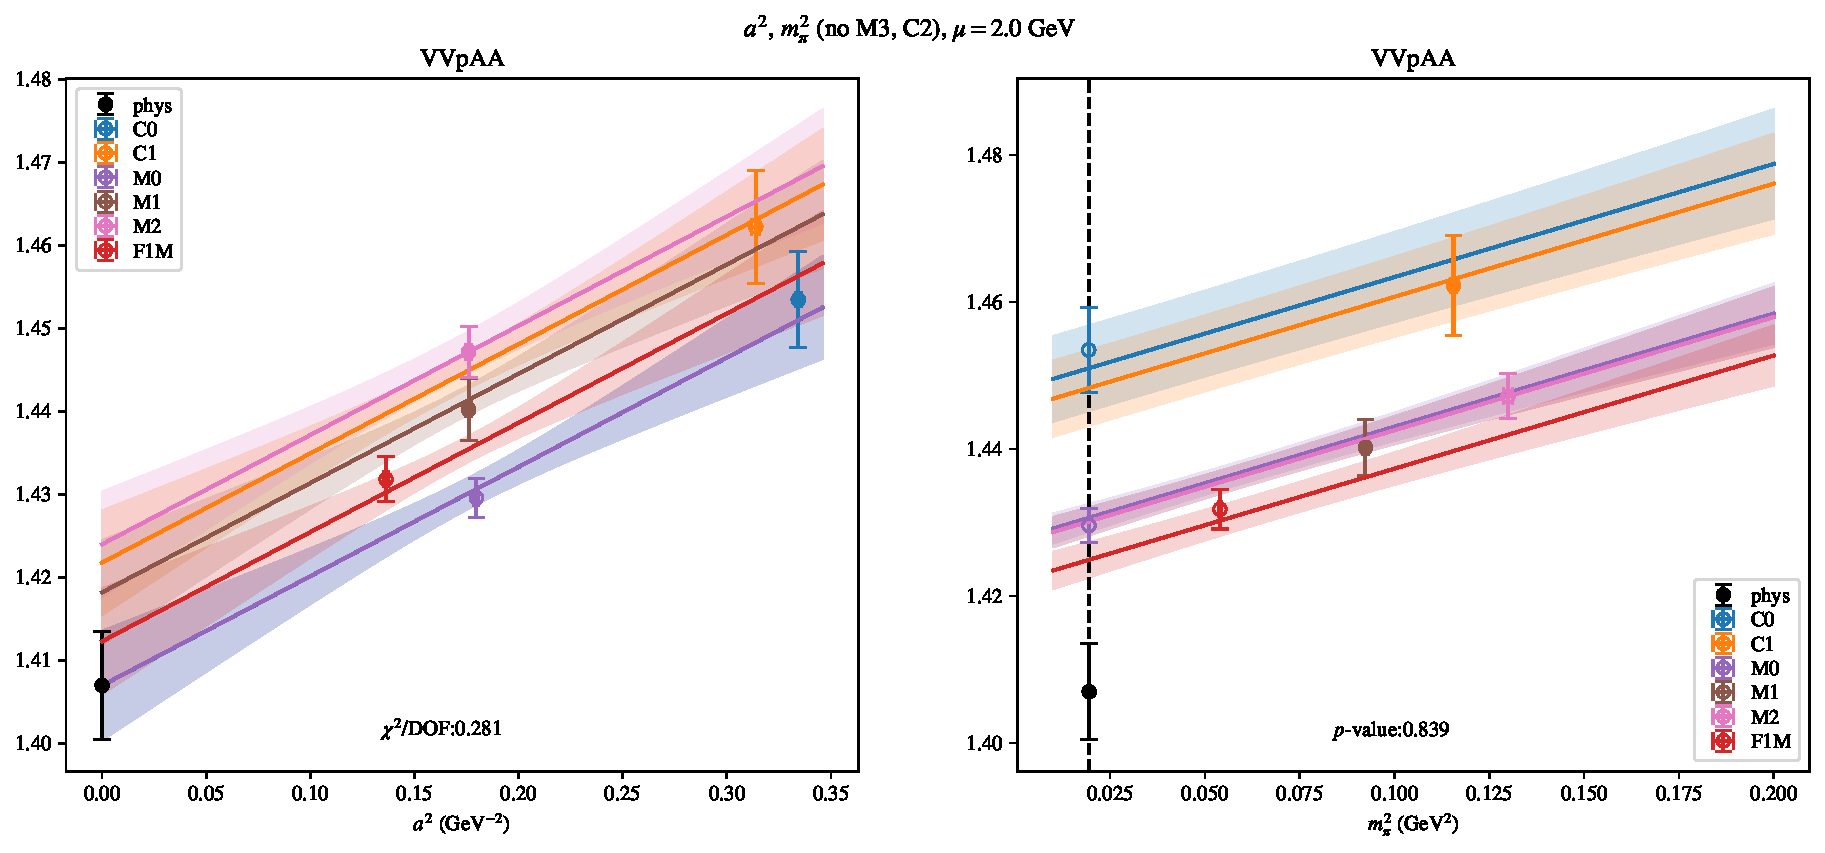
\includepdf[link, pages=-]{VVpAA/NPR/a2m2mcut_20.pdf}
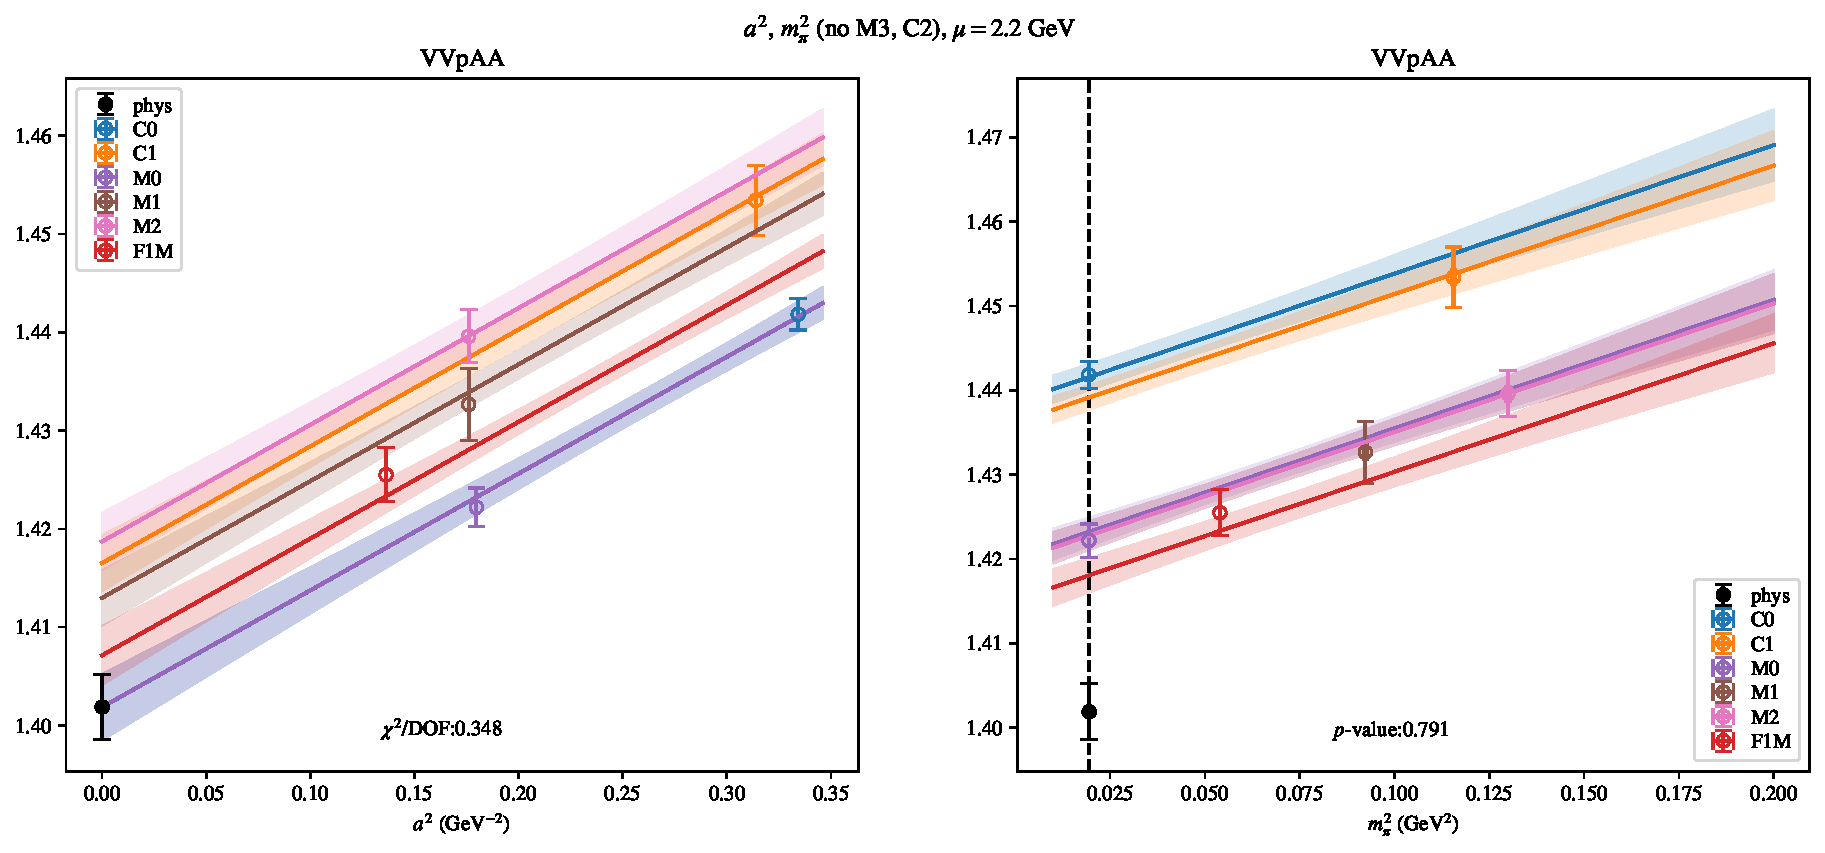
\includepdf[link, pages=-]{VVpAA/NPR/a2m2mcut_22.pdf}
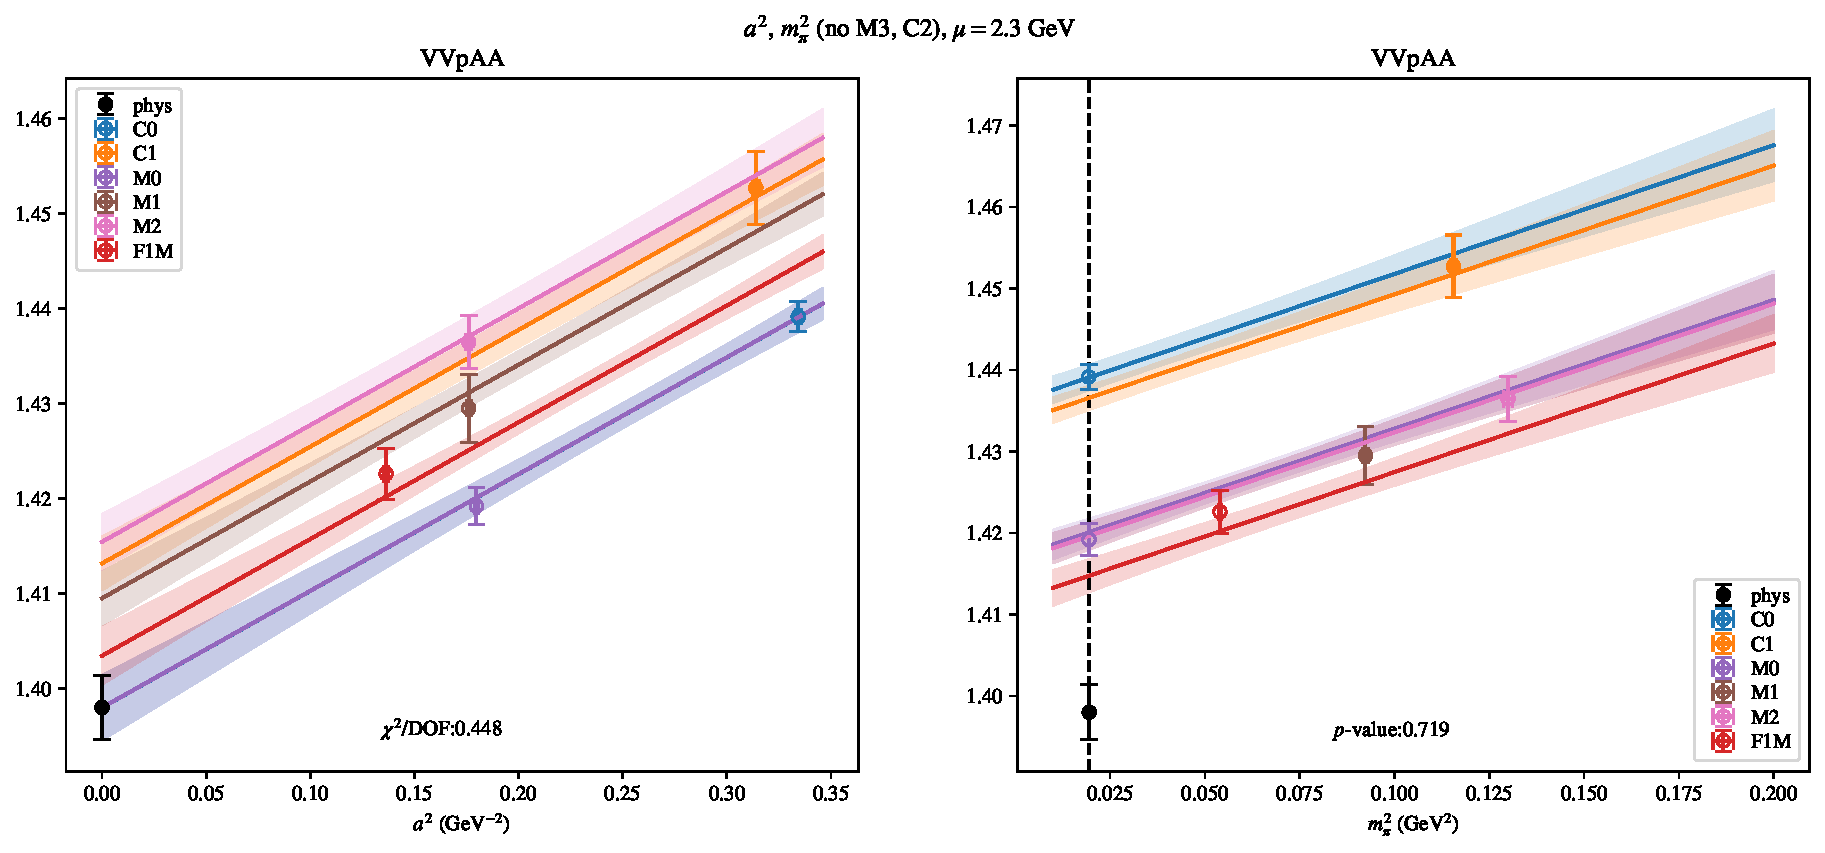
\includepdf[link, pages=-]{VVpAA/NPR/a2m2mcut_23.pdf}
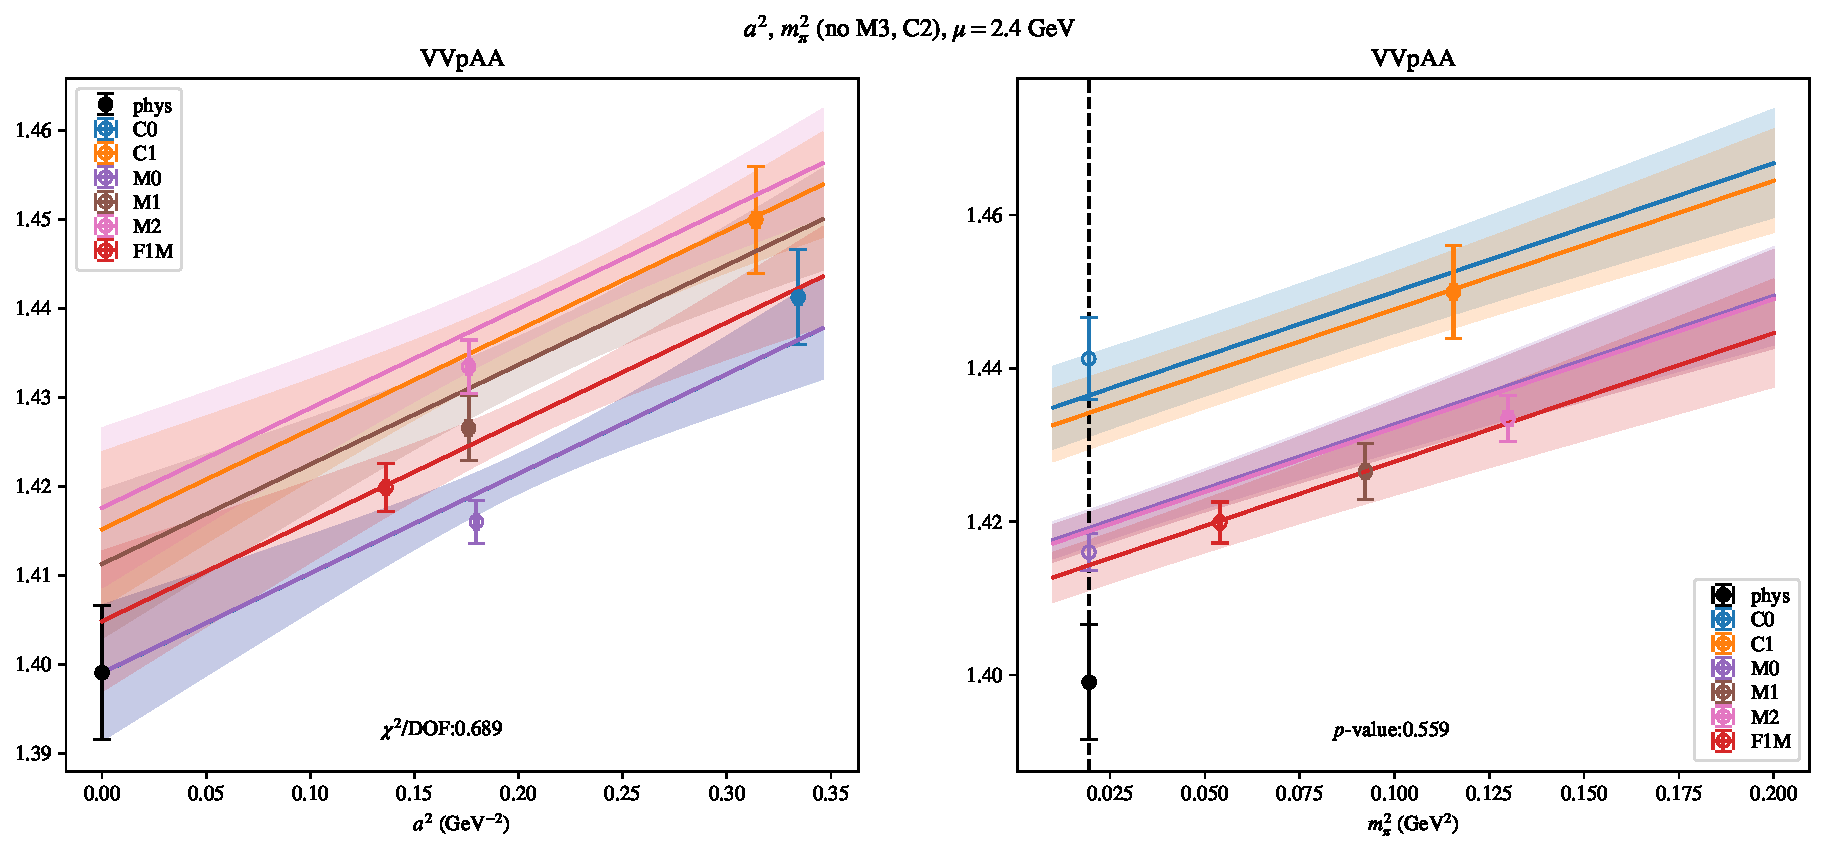
\includepdf[link, pages=-]{VVpAA/NPR/a2m2mcut_24.pdf}
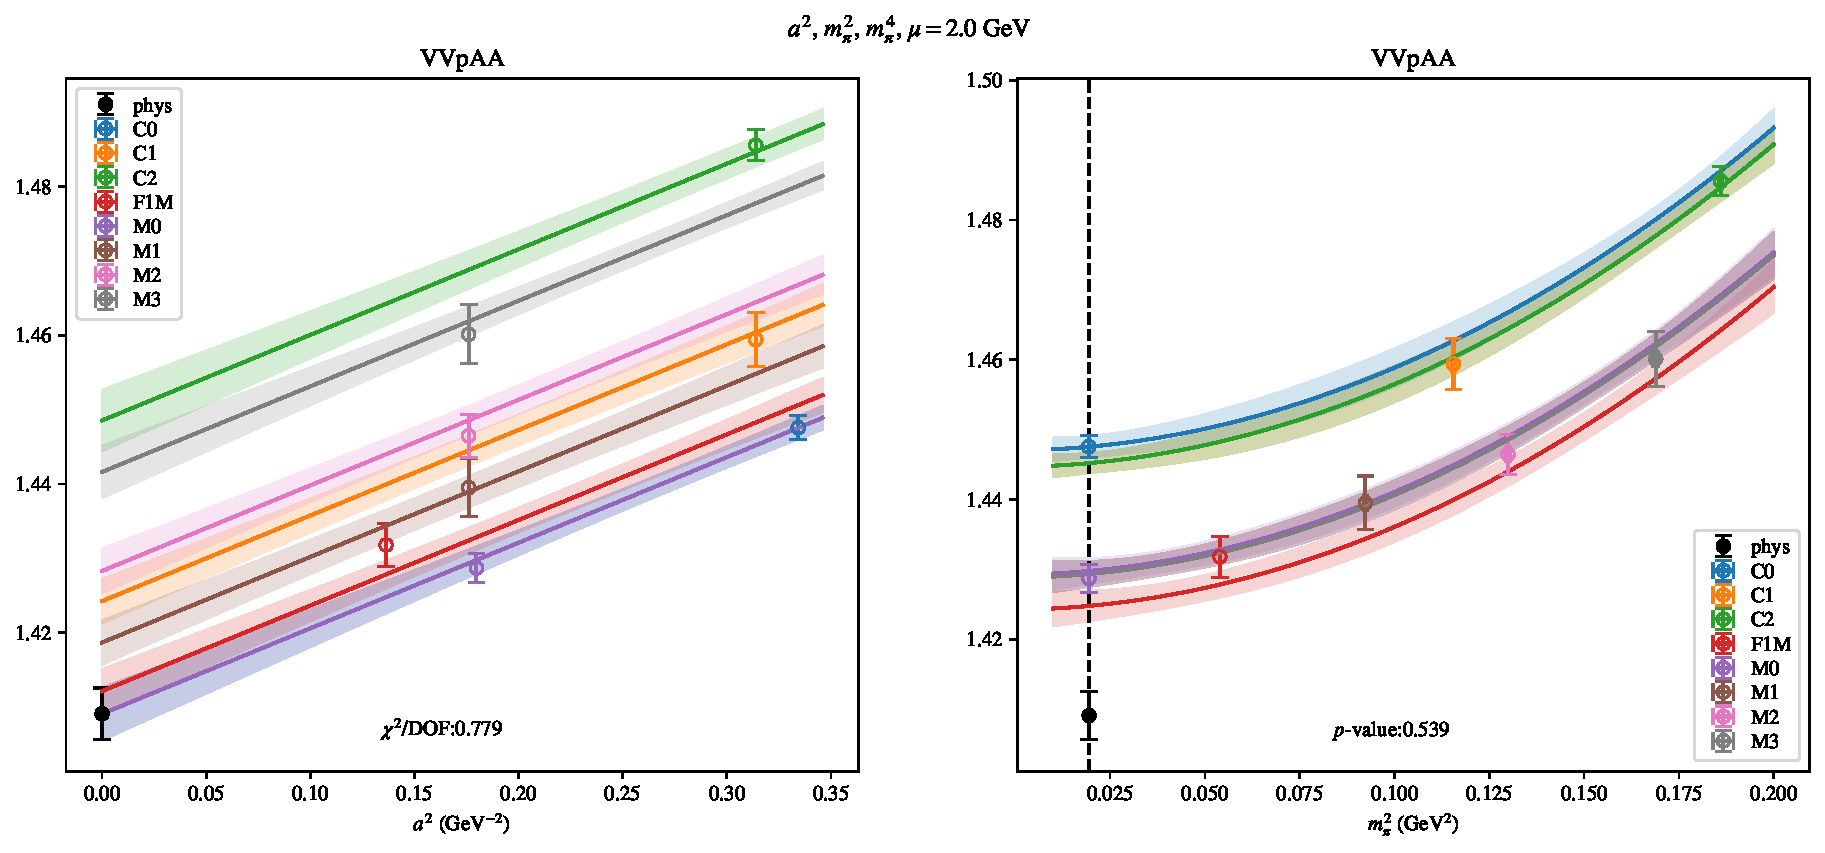
\includepdf[link, pages=-]{VVpAA/NPR/a2m2m4_20.pdf}
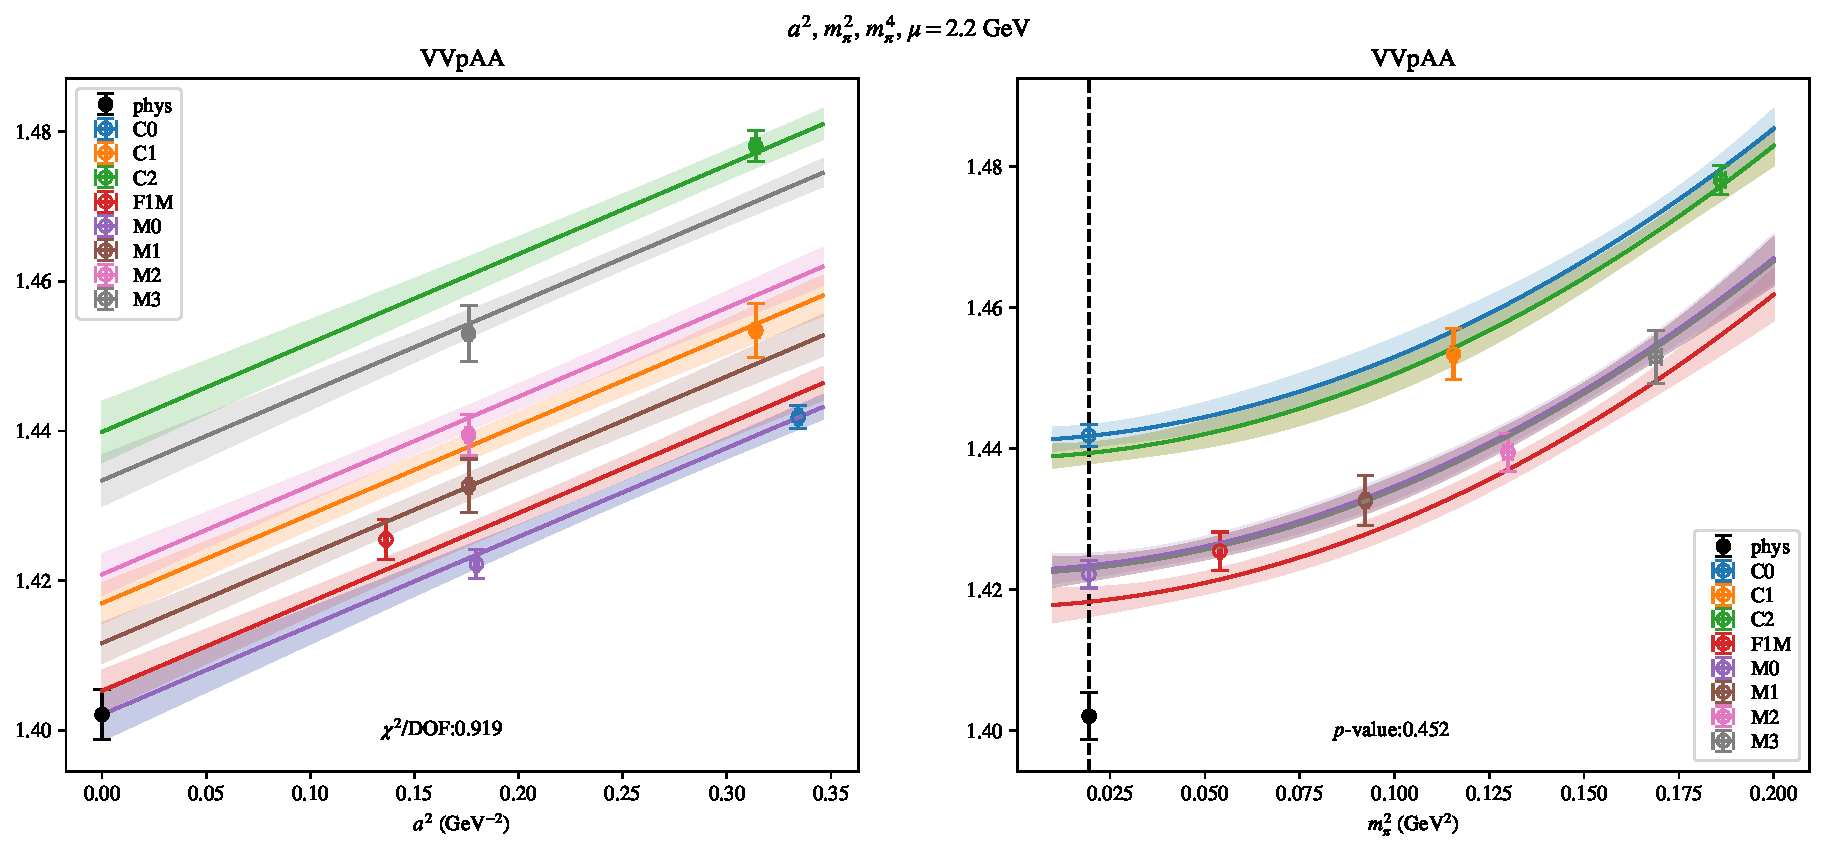
\includepdf[link, pages=-]{VVpAA/NPR/a2m2m4_22.pdf}
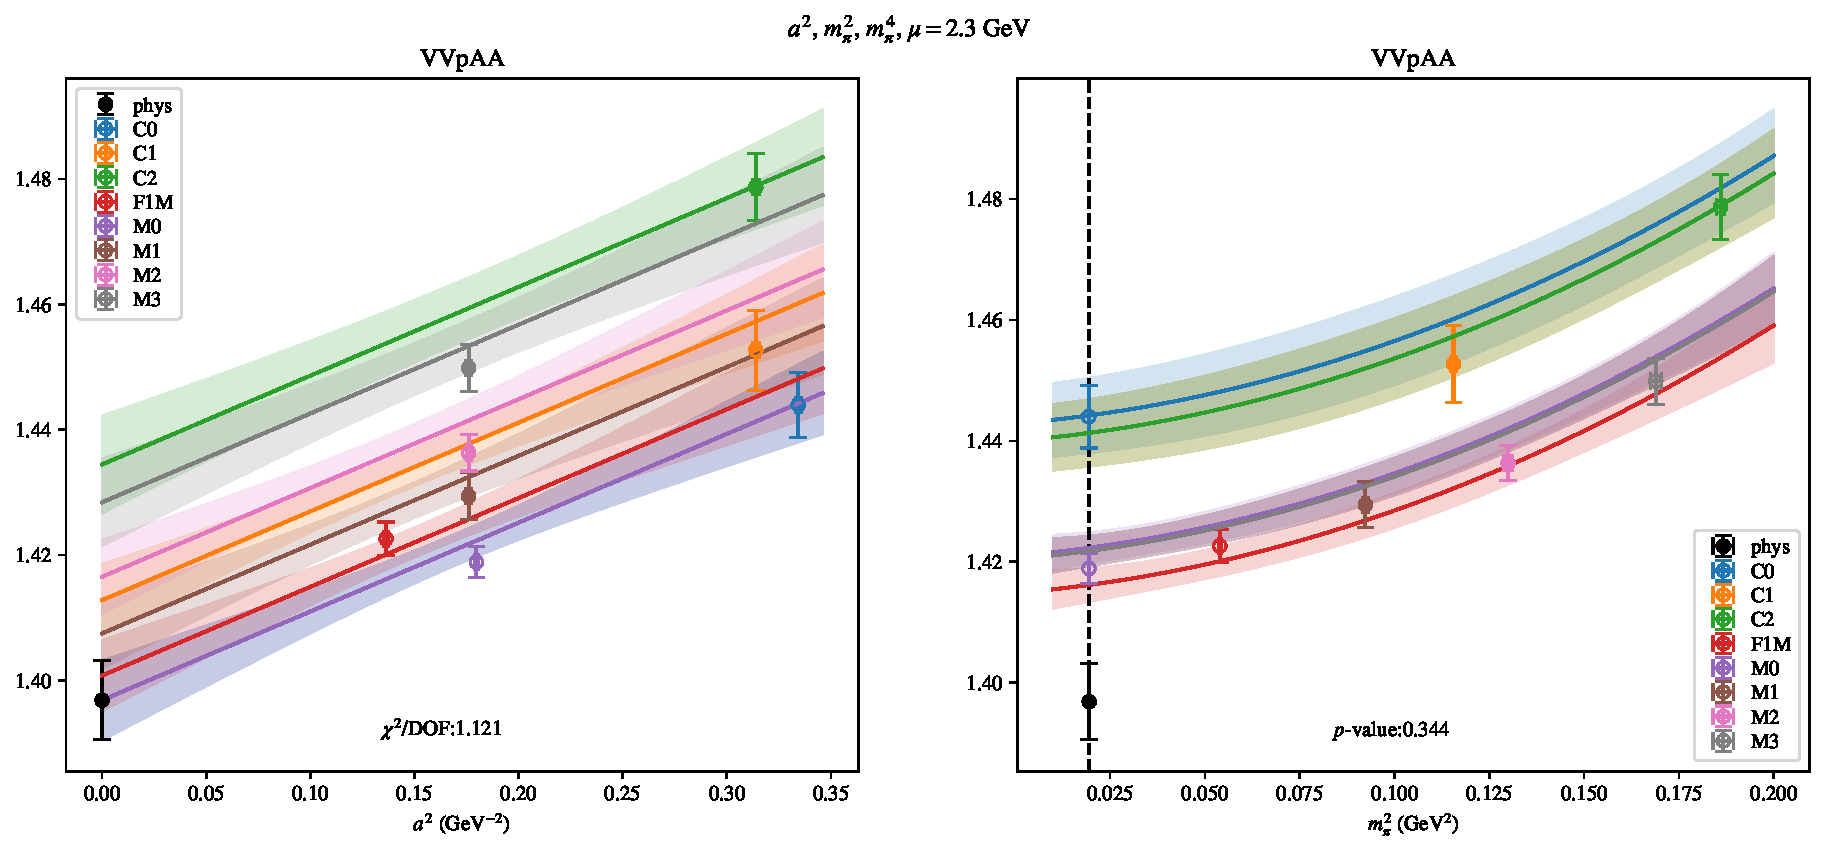
\includepdf[link, pages=-]{VVpAA/NPR/a2m2m4_23.pdf}
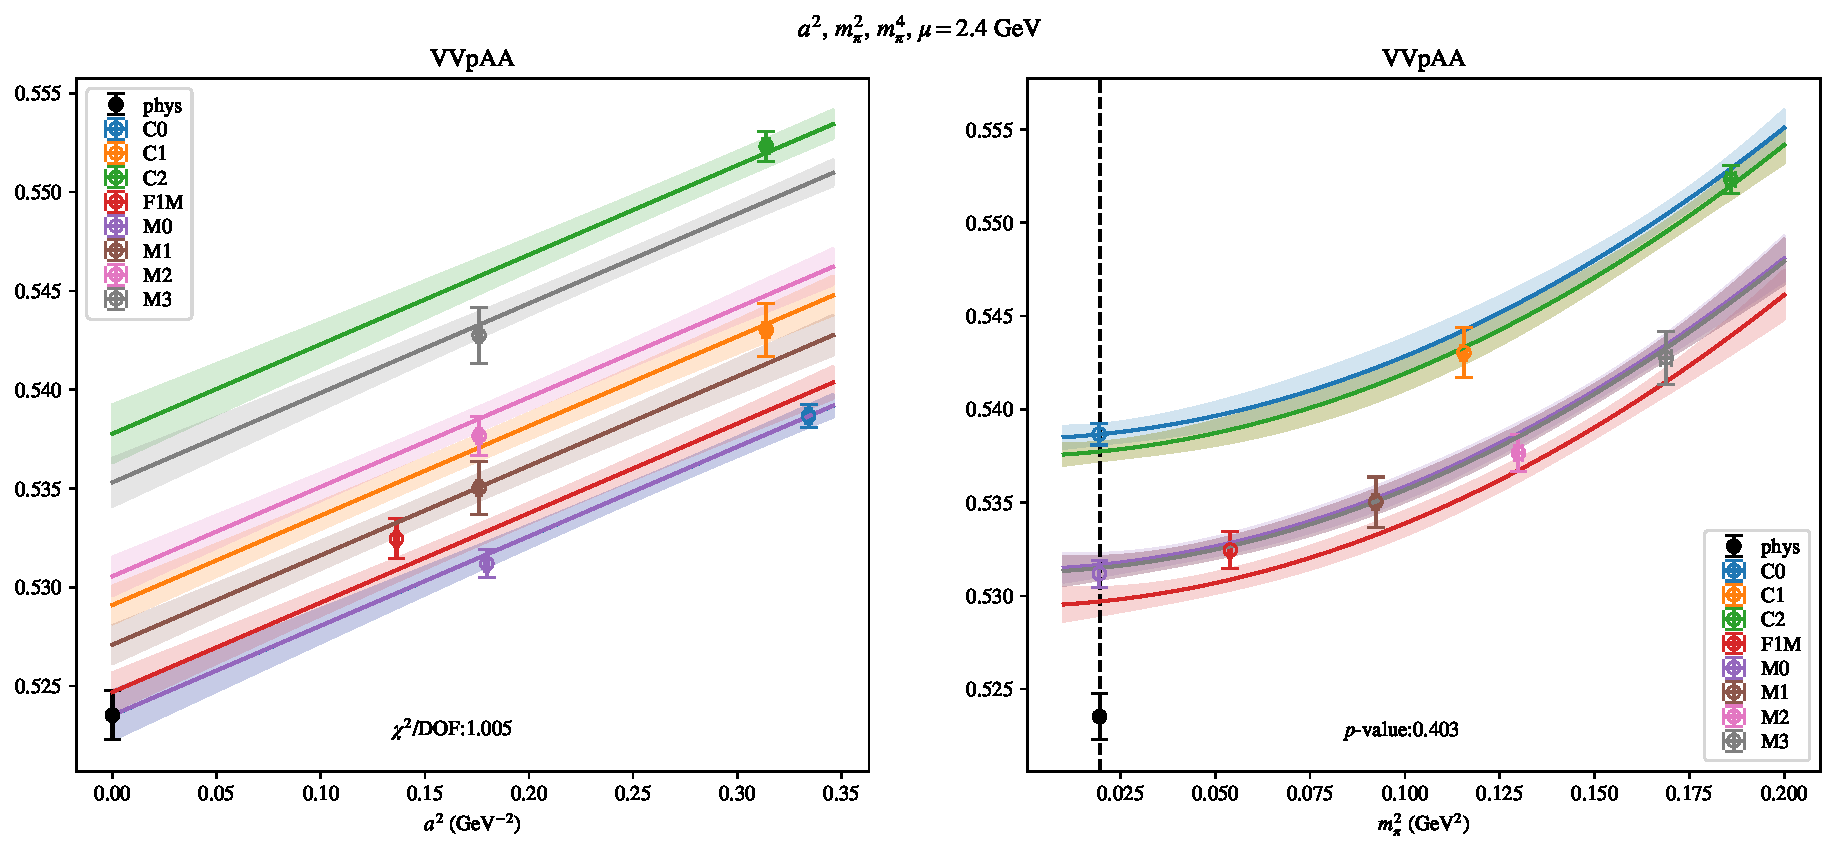
\includepdf[link, pages=-]{VVpAA/NPR/a2m2m4_24.pdf}
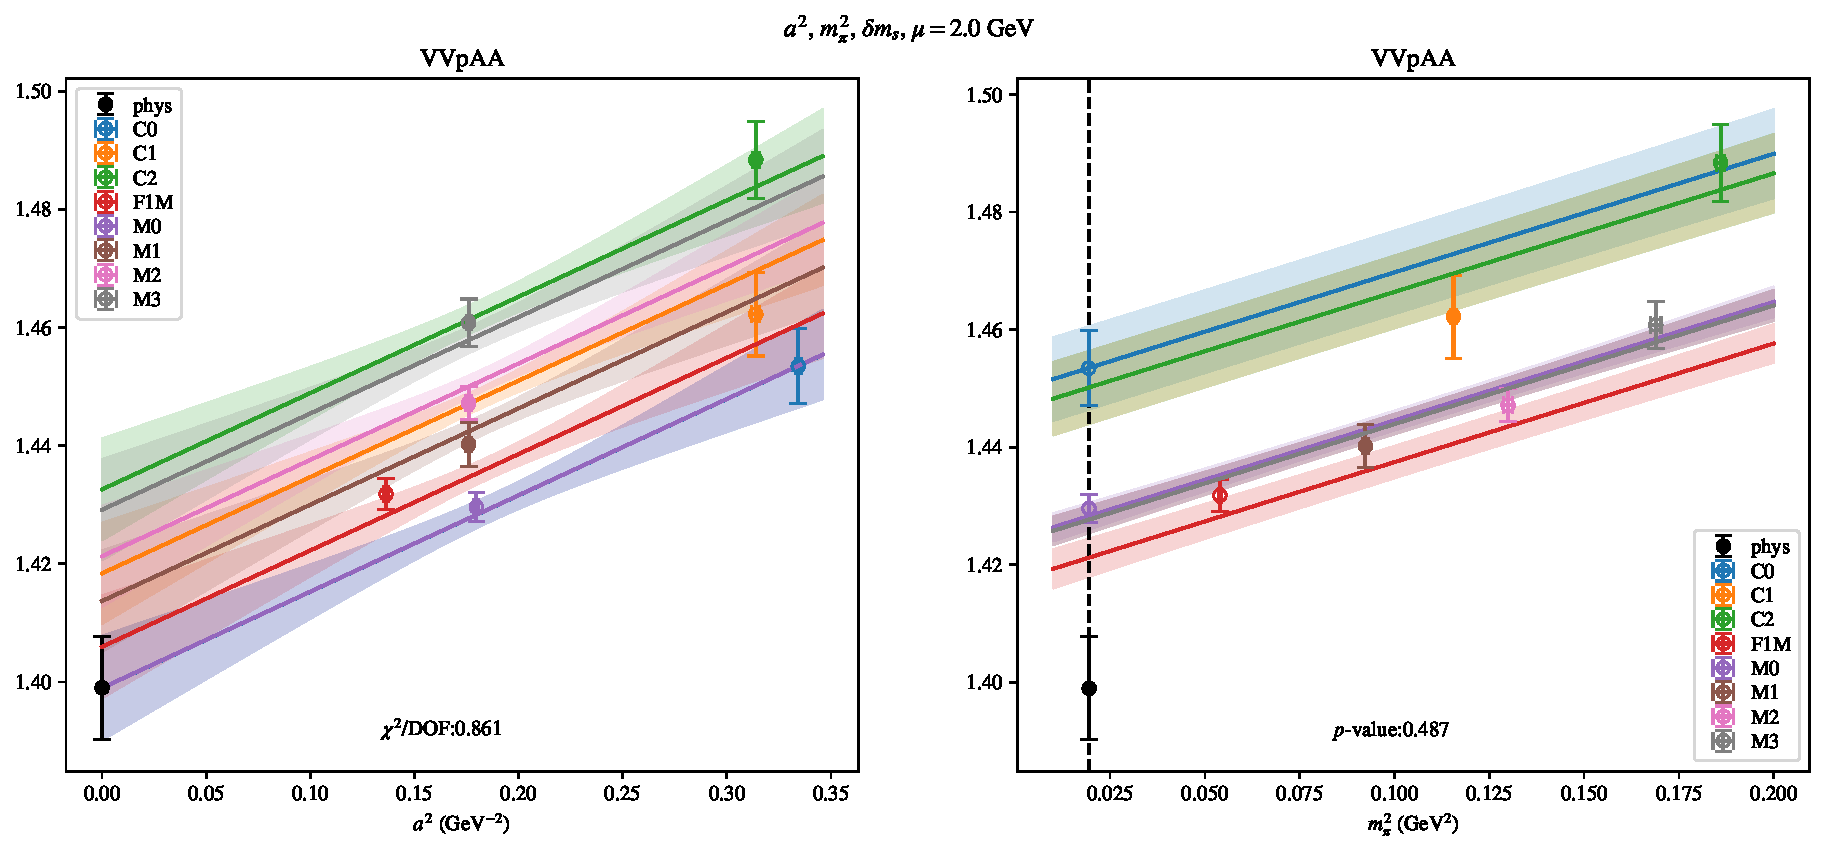
\includepdf[link, pages=-]{VVpAA/NPR/a2m2delm_20.pdf}
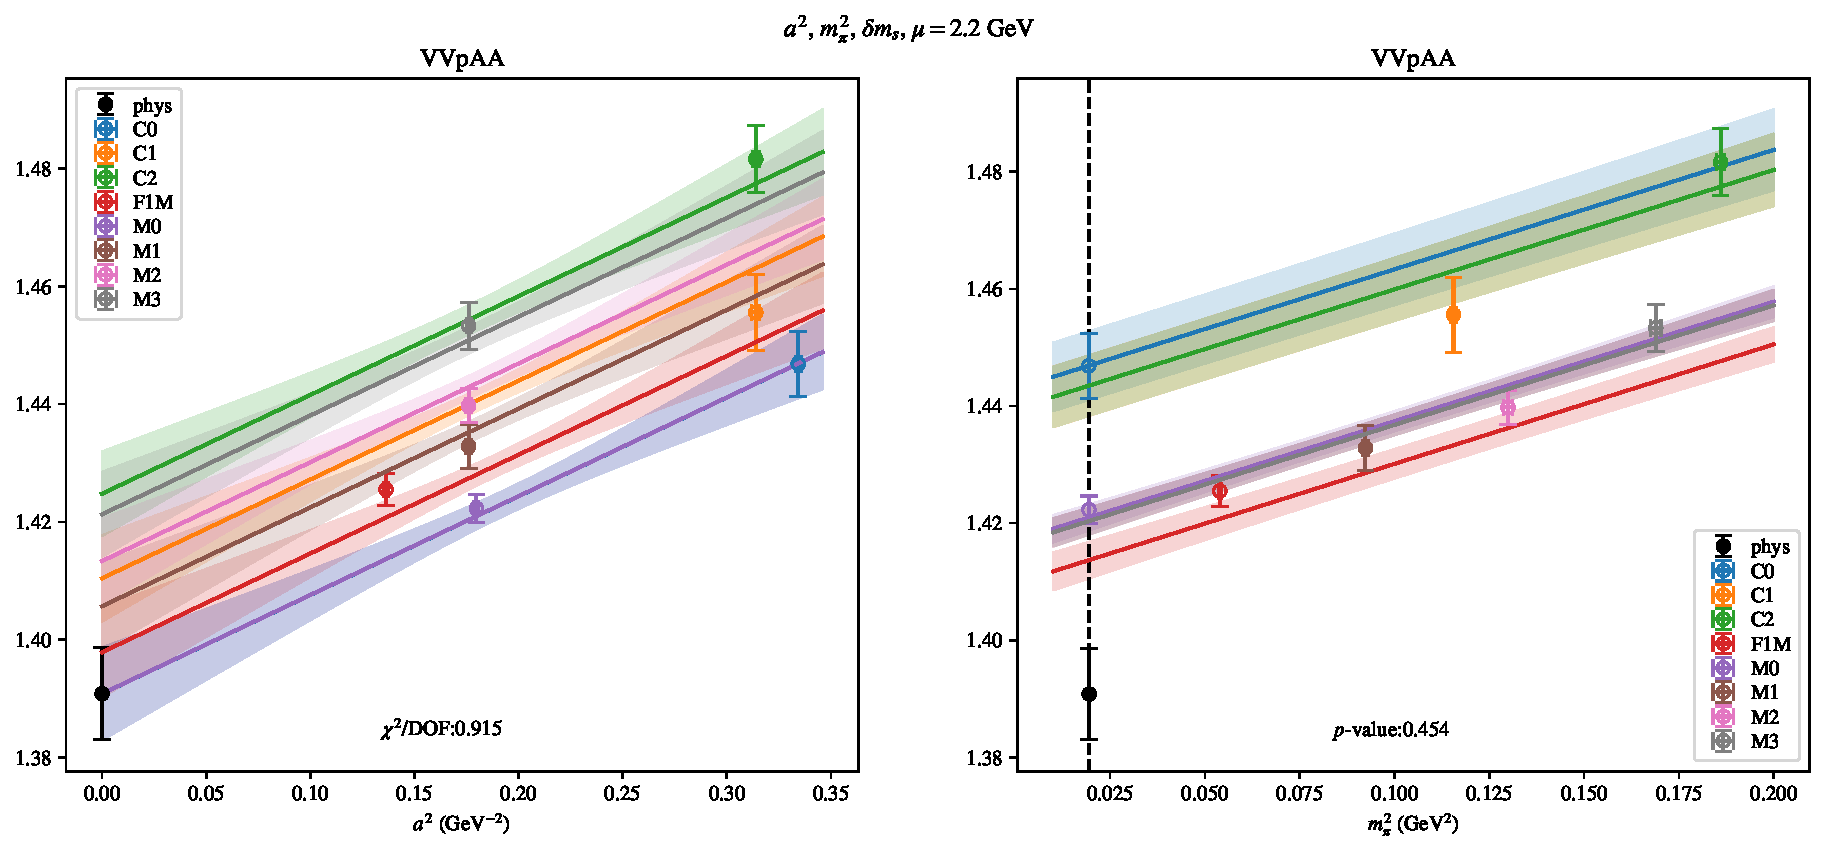
\includepdf[link, pages=-]{VVpAA/NPR/a2m2delm_22.pdf}
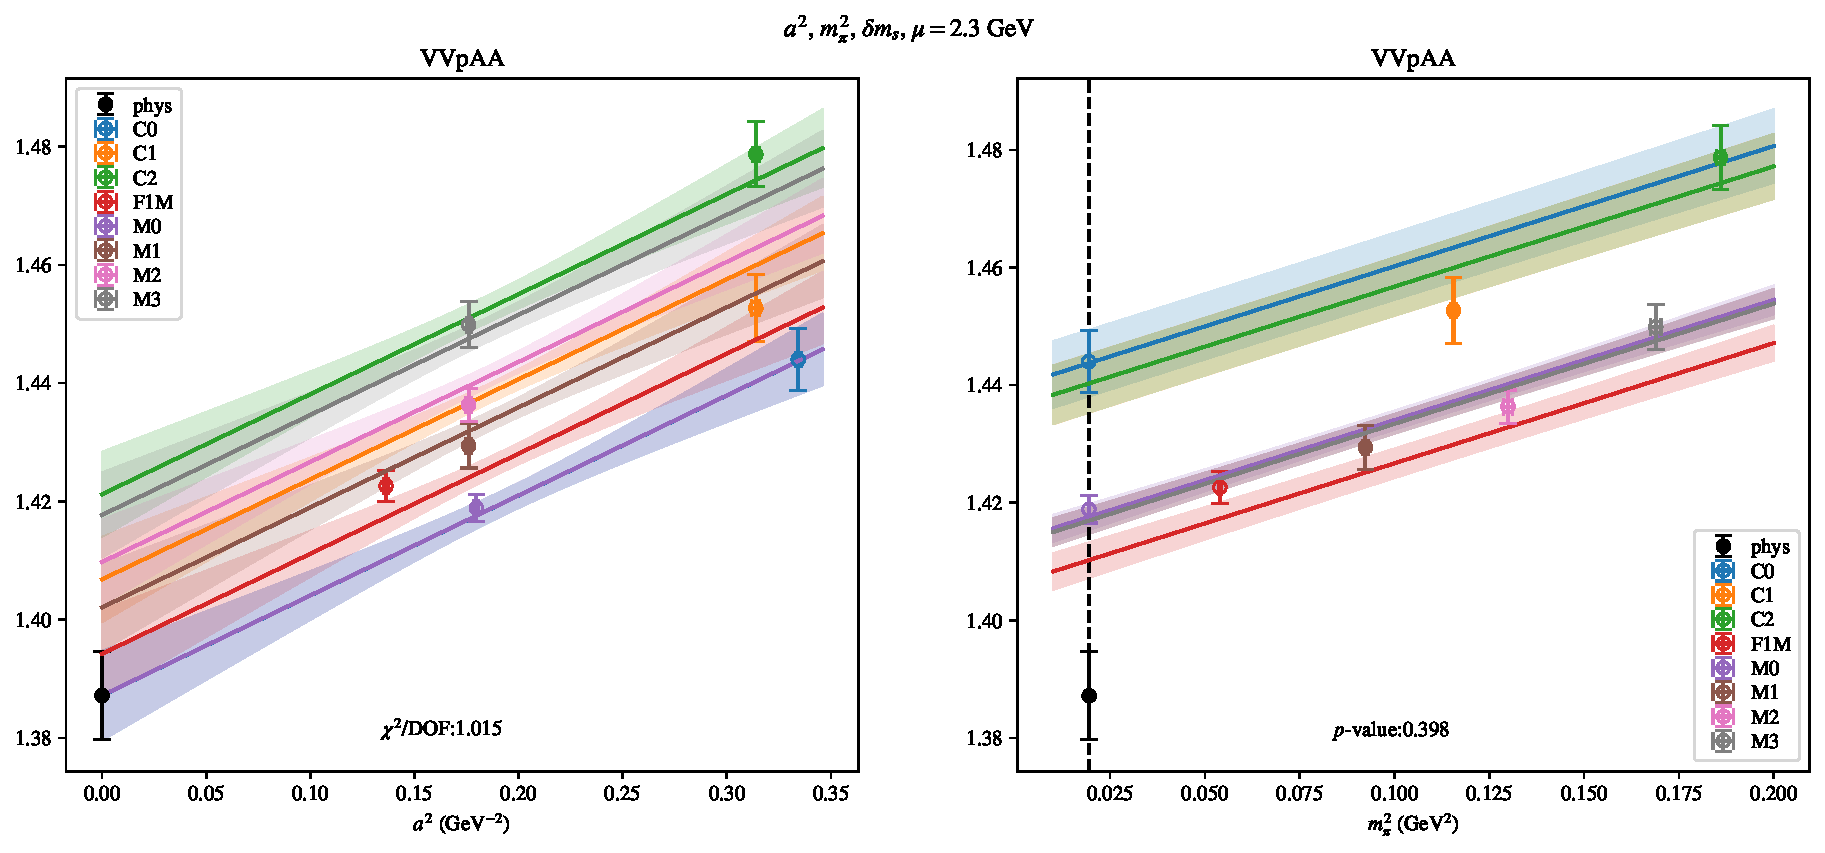
\includepdf[link, pages=-]{VVpAA/NPR/a2m2delm_23.pdf}
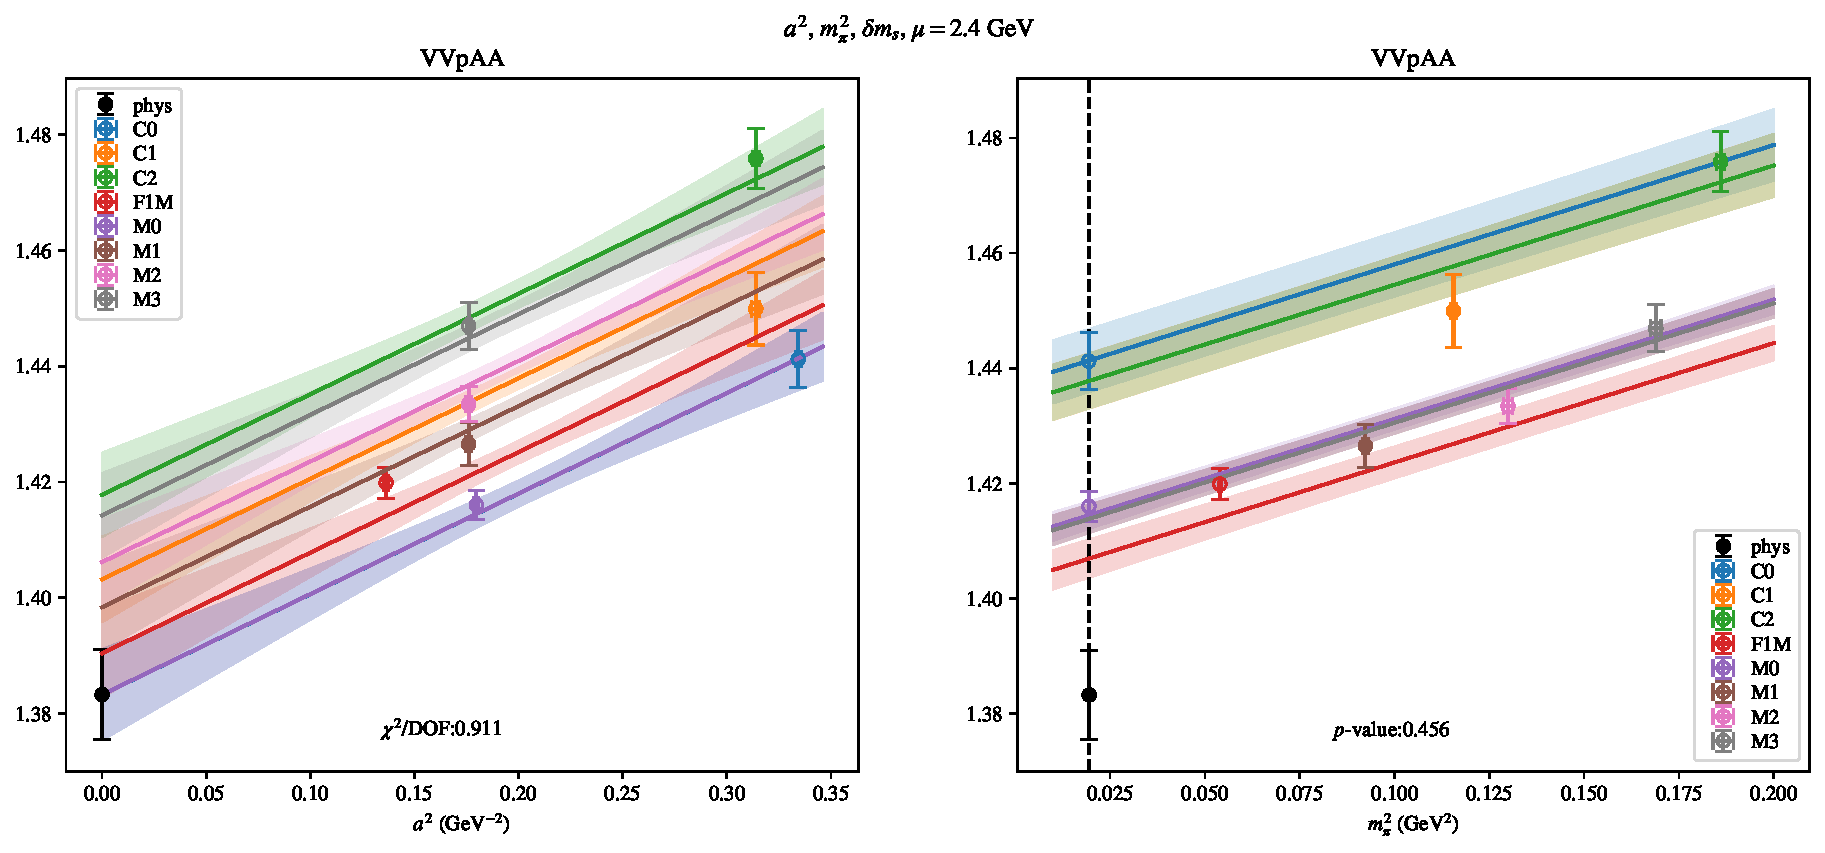
\includepdf[link, pages=-]{VVpAA/NPR/a2m2delm_24.pdf}
\clearpage
\section{$\mathcal{B}_2$}
\begin{table}[h!]
\begin{center}
\begin{tabular}{|c|c|c|c|c|c|c|}
\hline
$\mu$ (GeV) & $a^2$, $m_\pi^2$& $a^2$, $m_\pi^2$ (no C)& $a^2$, $m_\pi^2$, $a^4$& $a^2$, $m_\pi^2$ (no M3, C2)& $a^2$, $m_\pi^2$, $m_\pi^4$& $a^2$, $m_\pi^2$, $\delta m_s$\\
\hline
2.0& \hyperlink{VVmAA/NPR/a2m2_20.pdf.1}{\textbf{-0.993(24)}: 12.132 (0.0)} & \hyperlink{VVmAA/NPR/a2m2noC_20.pdf.1}{\textbf{-0.91(12)}: 0.361 (0.697)} & \hyperlink{VVmAA/NPR/a2a4m2_20.pdf.1}{\textbf{-0.88(13)}: 1.033 (0.388)} & \hyperlink{VVmAA/NPR/a2m2mcut_20.pdf.1}{\textbf{-0.993(23)}: 17.677 (0.0)} & \hyperlink{VVmAA/NPR/a2m2m4_20.pdf.1}{\textbf{-0.995(24)}: 9.387 (0.0)} & \hyperlink{VVmAA/NPR/a2m2delm_20.pdf.1}{\textbf{-0.997(26)}: 0.507 (0.731)}\\
2.2& \hyperlink{VVmAA/NPR/a2m2_22.pdf.1}{\textbf{-1.006(17)}: 10.074 (0.0)} & \hyperlink{VVmAA/NPR/a2m2noC_22.pdf.1}{\textbf{-0.947(91)}: 1.166 (0.312)} & \hyperlink{VVmAA/NPR/a2a4m2_22.pdf.1}{\textbf{-0.91(13)}: 1.271 (0.279)} & \hyperlink{VVmAA/NPR/a2m2mcut_22.pdf.1}{\textbf{-1.007(20)}: 14.486 (0.0)} & \hyperlink{VVmAA/NPR/a2m2m4_22.pdf.1}{\textbf{-1.008(19)}: 8.173 (0.0)} & \hyperlink{VVmAA/NPR/a2m2delm_22.pdf.1}{\textbf{-1.009(17)}: 1.363 (0.244)}\\
2.3& \hyperlink{VVmAA/NPR/a2m2_23.pdf.1}{\textbf{-1.011(14)}: 10.487 (0.0)} & \hyperlink{VVmAA/NPR/a2m2noC_23.pdf.1}{\textbf{-0.955(93)}: 1.503 (0.222)} & \hyperlink{VVmAA/NPR/a2a4m2_23.pdf.1}{\textbf{-0.91(12)}: 1.24 (0.291)} & \hyperlink{VVmAA/NPR/a2m2mcut_23.pdf.1}{\textbf{-1.013(17)}: 15.351 (0.0)} & \hyperlink{VVmAA/NPR/a2m2m4_23.pdf.1}{\textbf{-1.014(15)}: 8.814 (0.0)} & \hyperlink{VVmAA/NPR/a2m2delm_23.pdf.1}{\textbf{-1.014(15)}: 1.75 (0.136)}\\
2.4& \hyperlink{VVmAA/NPR/a2m2_24.pdf.1}{\textbf{-1.016(14)}: 9.724 (0.0)} & \hyperlink{VVmAA/NPR/a2m2noC_24.pdf.1}{\textbf{-0.963(90)}: 1.729 (0.178)} & \hyperlink{VVmAA/NPR/a2a4m2_24.pdf.1}{\textbf{-0.92(12)}: 1.515 (0.195)} & \hyperlink{VVmAA/NPR/a2m2mcut_24.pdf.1}{\textbf{-1.017(16)}: 14.2 (0.0)} & \hyperlink{VVmAA/NPR/a2m2m4_24.pdf.1}{\textbf{-1.018(15)}: 8.365 (0.0)} & \hyperlink{VVmAA/NPR/a2m2delm_24.pdf.1}{\textbf{-1.018(14)}: 1.871 (0.112)}\\
\hline
\end{tabular}
\caption{Physical point value from chiral and continuum extrapolation at renormalisation scale $\mu$. Entries are \textbf{value(error)}: $\chi^2/\text{DOF}$ ($p$-value).}
\end{center}
\end{table}
\begin{table}[h!]
\begin{center}
\begin{tabular}{|c c|c|c|c|c|c|c|}
\hline
$\mu$ (GeV) &  & $a^2$, $m_\pi^2$& $a^2$, $m_\pi^2$ (no C)& $a^2$, $m_\pi^2$, $a^4$& $a^2$, $m_\pi^2$ (no M3, C2)& $a^2$, $m_\pi^2$, $m_\pi^4$& $a^2$, $m_\pi^2$, $\delta m_s$\\
\hline
\multirow{3}{0.5in}{2.0} & $\alpha$ & -0.18(10)& 0.283(76)& 0.90(14)& -0.191(98)& -0.19(10)& -0.20(10)\\
 & $\beta$ & 0.00148(34)& 0.00272(77)& 0.00160(38)& 0.00055(48)& -0.004(10)& 0.00130(34)\\
 & $\gamma$ &  &  & -2.2(30)&  & 0.000540(80)& 0.0192(26)\\
\hline
\multirow{3}{0.5in}{2.2} & $\alpha$ & -0.226(69)& 0.118(55)& 0.66(13)& -0.228(79)& -0.232(76)& -0.236(70)\\
 & $\beta$ & 0.00120(25)& 0.00125(61)& 0.00105(28)& 0.00036(47)& -0.003(11)& 0.00093(25)\\
 & $\gamma$ &  &  & -1.7(27)&  & 0.000397(90)& 0.0151(20)\\
\hline
\multirow{3}{0.5in}{2.3} & $\alpha$ & -0.245(56)& 0.076(55)& 0.63(13)& -0.249(67)& -0.252(61)& -0.254(56)\\
 & $\beta$ & 0.00127(25)& 0.00109(63)& 0.00113(28)& 0.00051(47)& -0.002(11)& 0.00099(24)\\
 & $\gamma$ &  &  & -1.7(26)&  & 0.000371(89)& 0.0144(20)\\
\hline
\multirow{3}{0.5in}{2.4} & $\alpha$ & -0.262(51)& 0.038(53)& 0.56(12)& -0.266(62)& -0.269(54)& -0.271(52)\\
 & $\beta$ & 0.00130(21)& 0.00111(56)& 0.00116(23)& 0.00063(40)& -0.002(10)& 0.00101(20)\\
 & $\gamma$ &  &  & -1.6(25)&  & 0.000327(83)& 0.0134(20)\\
\hline
\end{tabular}
\caption{Fit values of coefficients in $Q = Q_{phys} + \mathbf{\alpha} a^2 + \mathbf{\beta}\left(\frac{m_\pi^2}{f_\pi^2}-\frac{m_{\pi,PDG}^2}{f_\pi^2}\right) + \gamma(\ldots)$}
\end{center}
\end{table}
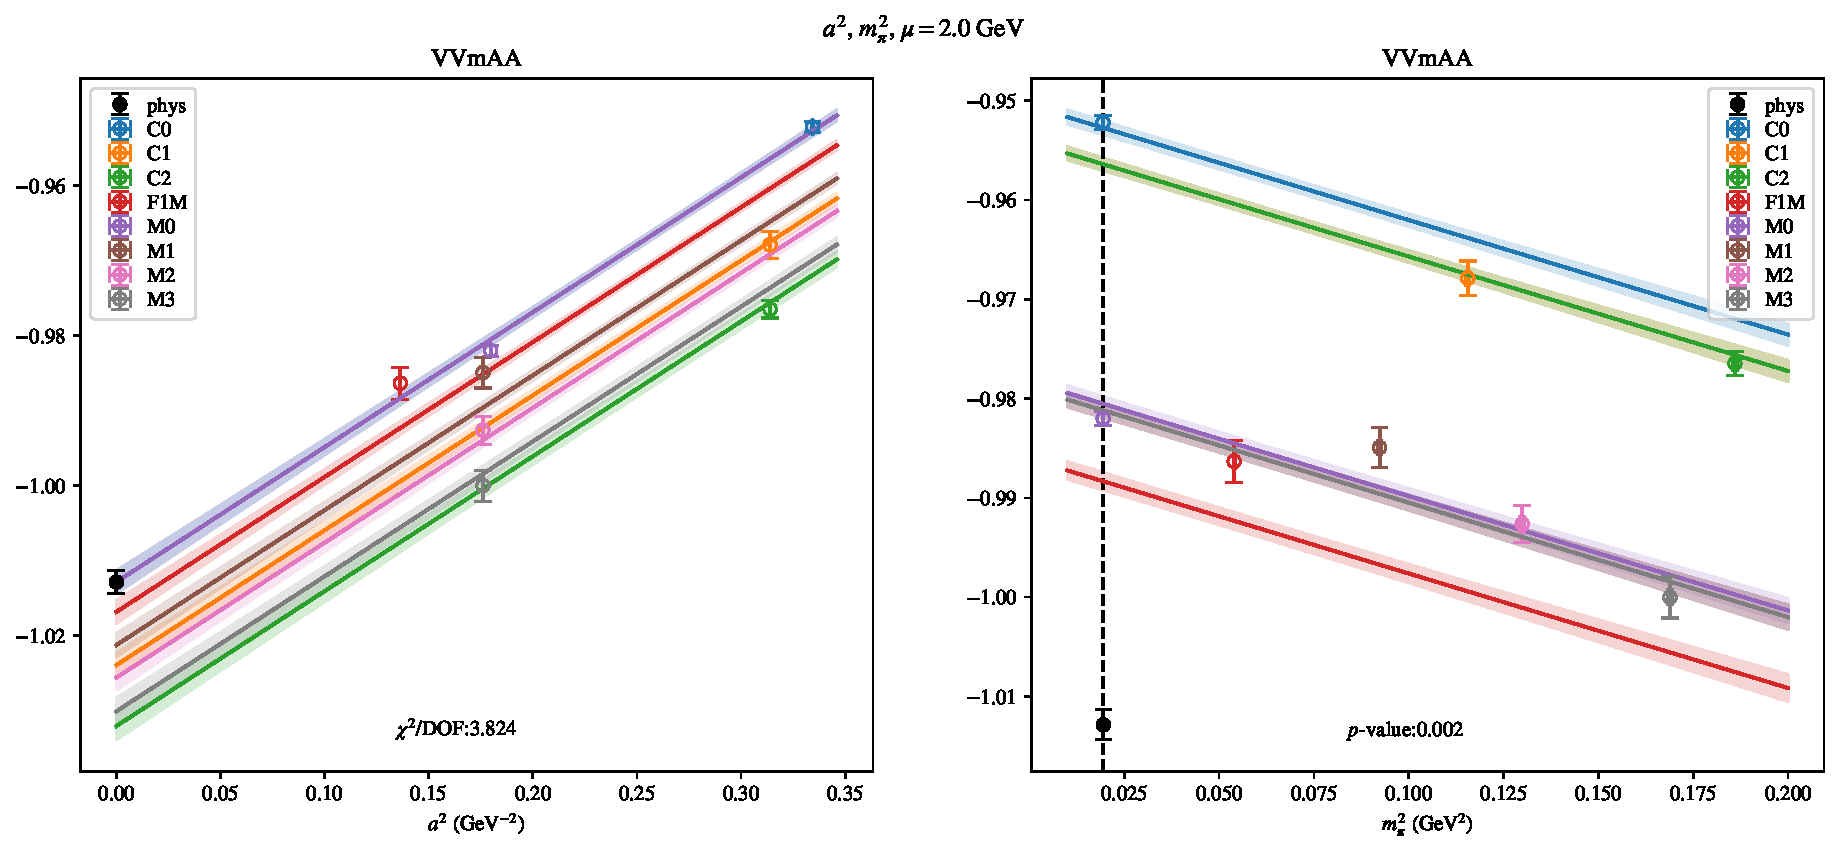
\includepdf[link, pages=-]{VVmAA/NPR/a2m2_20.pdf}
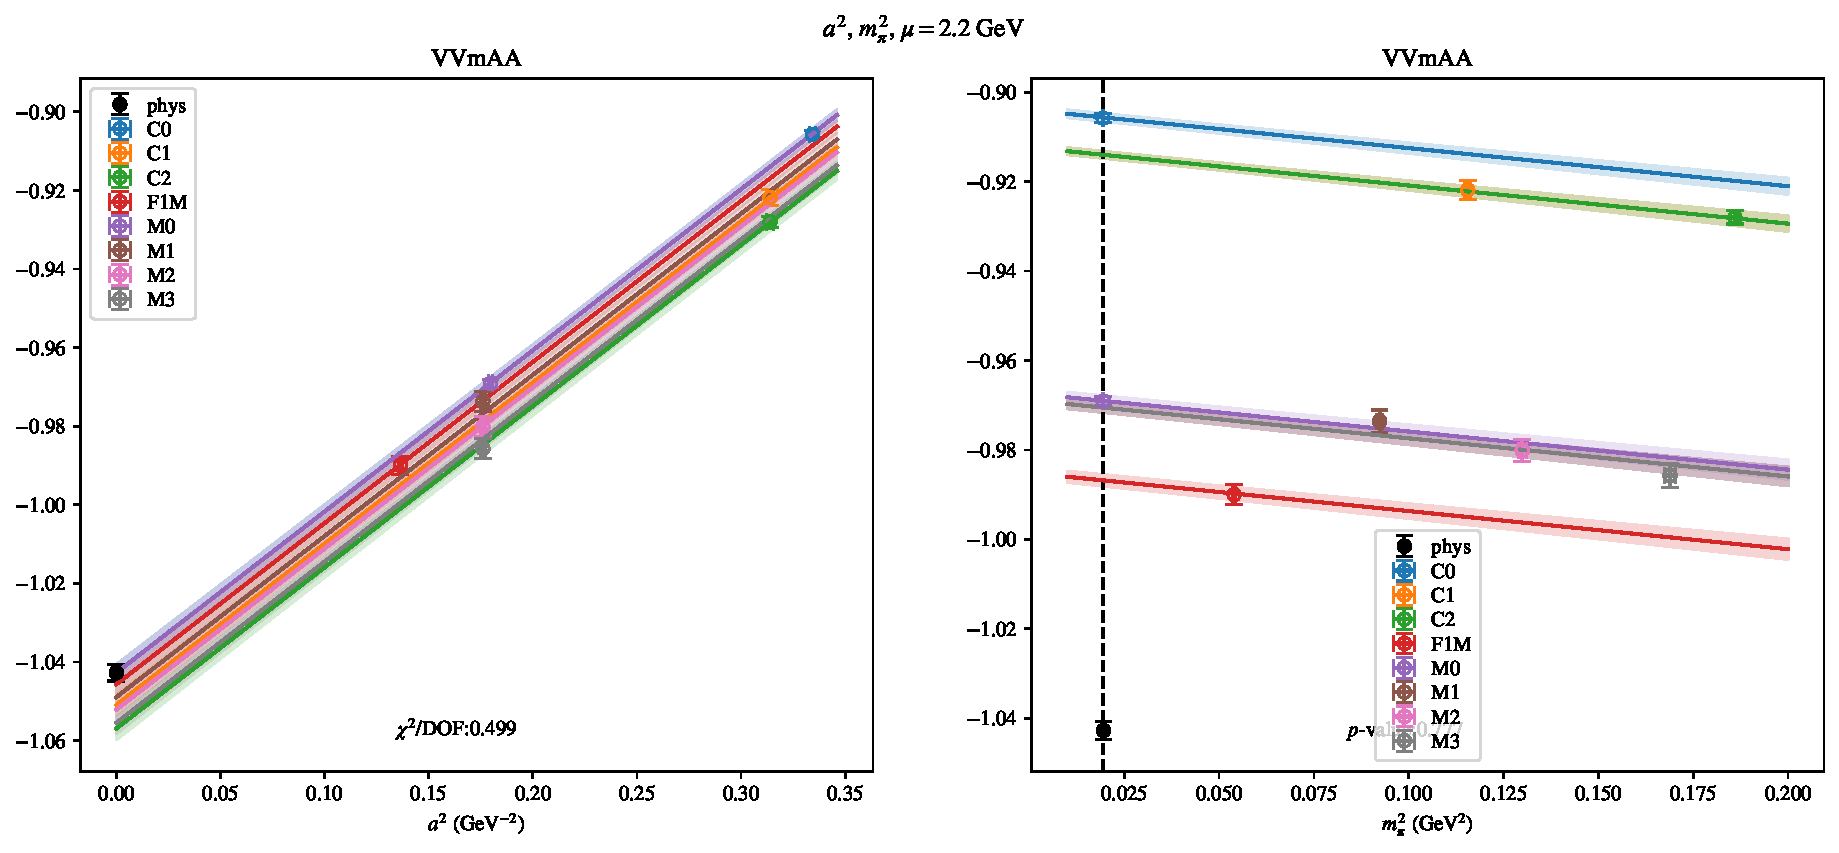
\includepdf[link, pages=-]{VVmAA/NPR/a2m2_22.pdf}
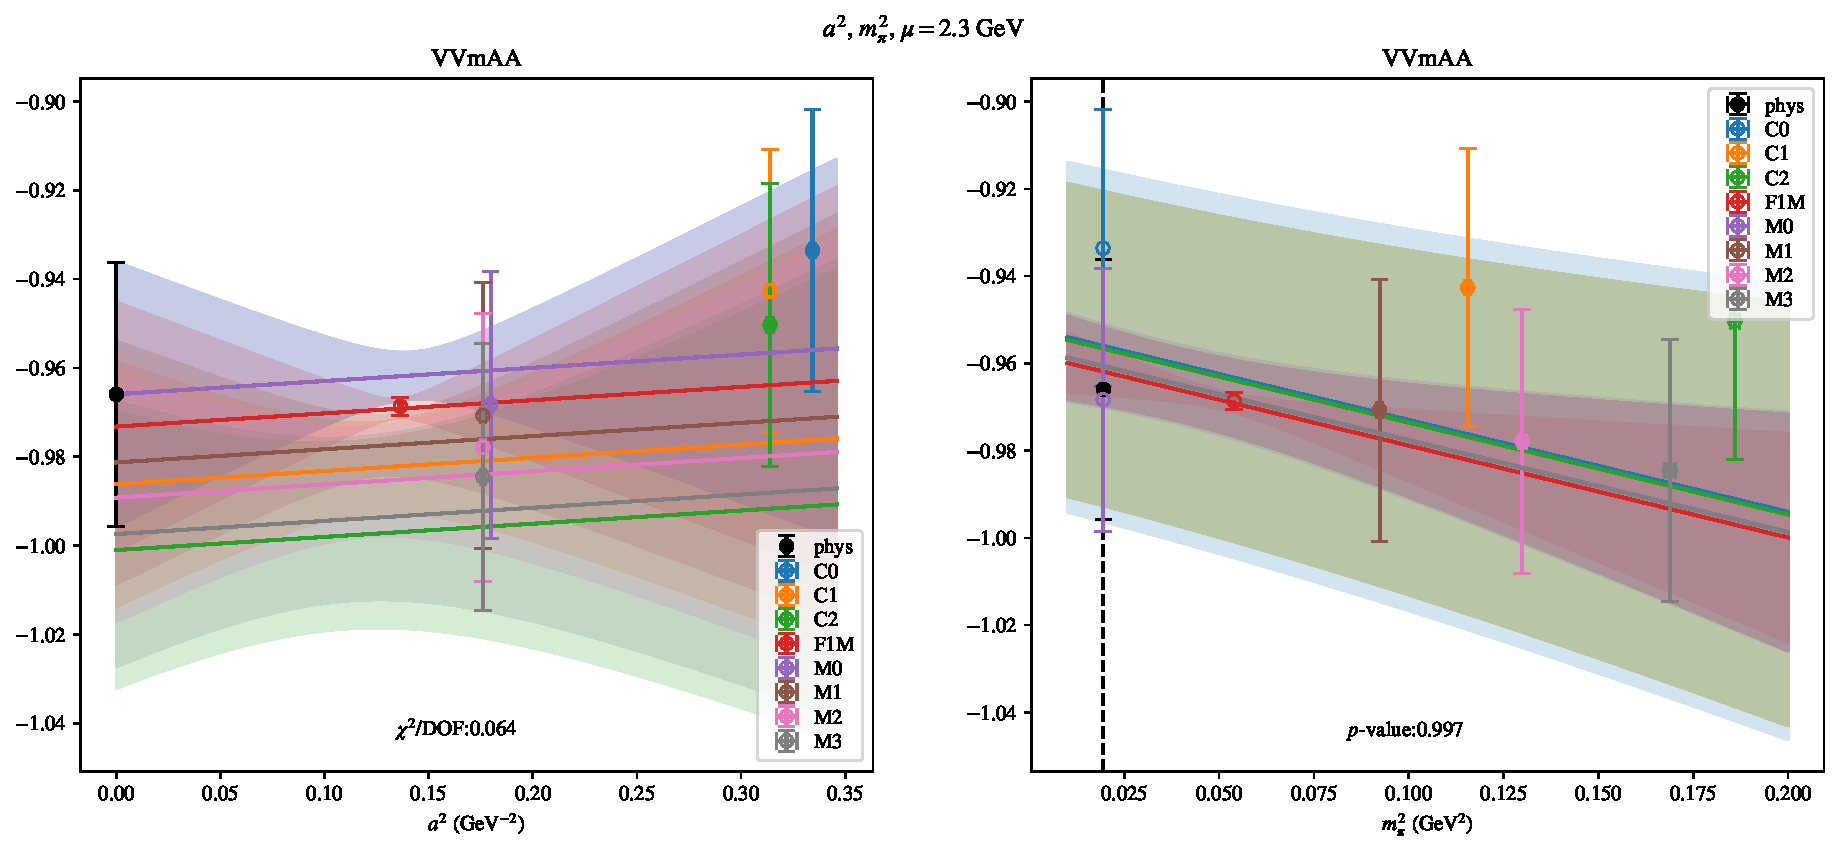
\includepdf[link, pages=-]{VVmAA/NPR/a2m2_23.pdf}
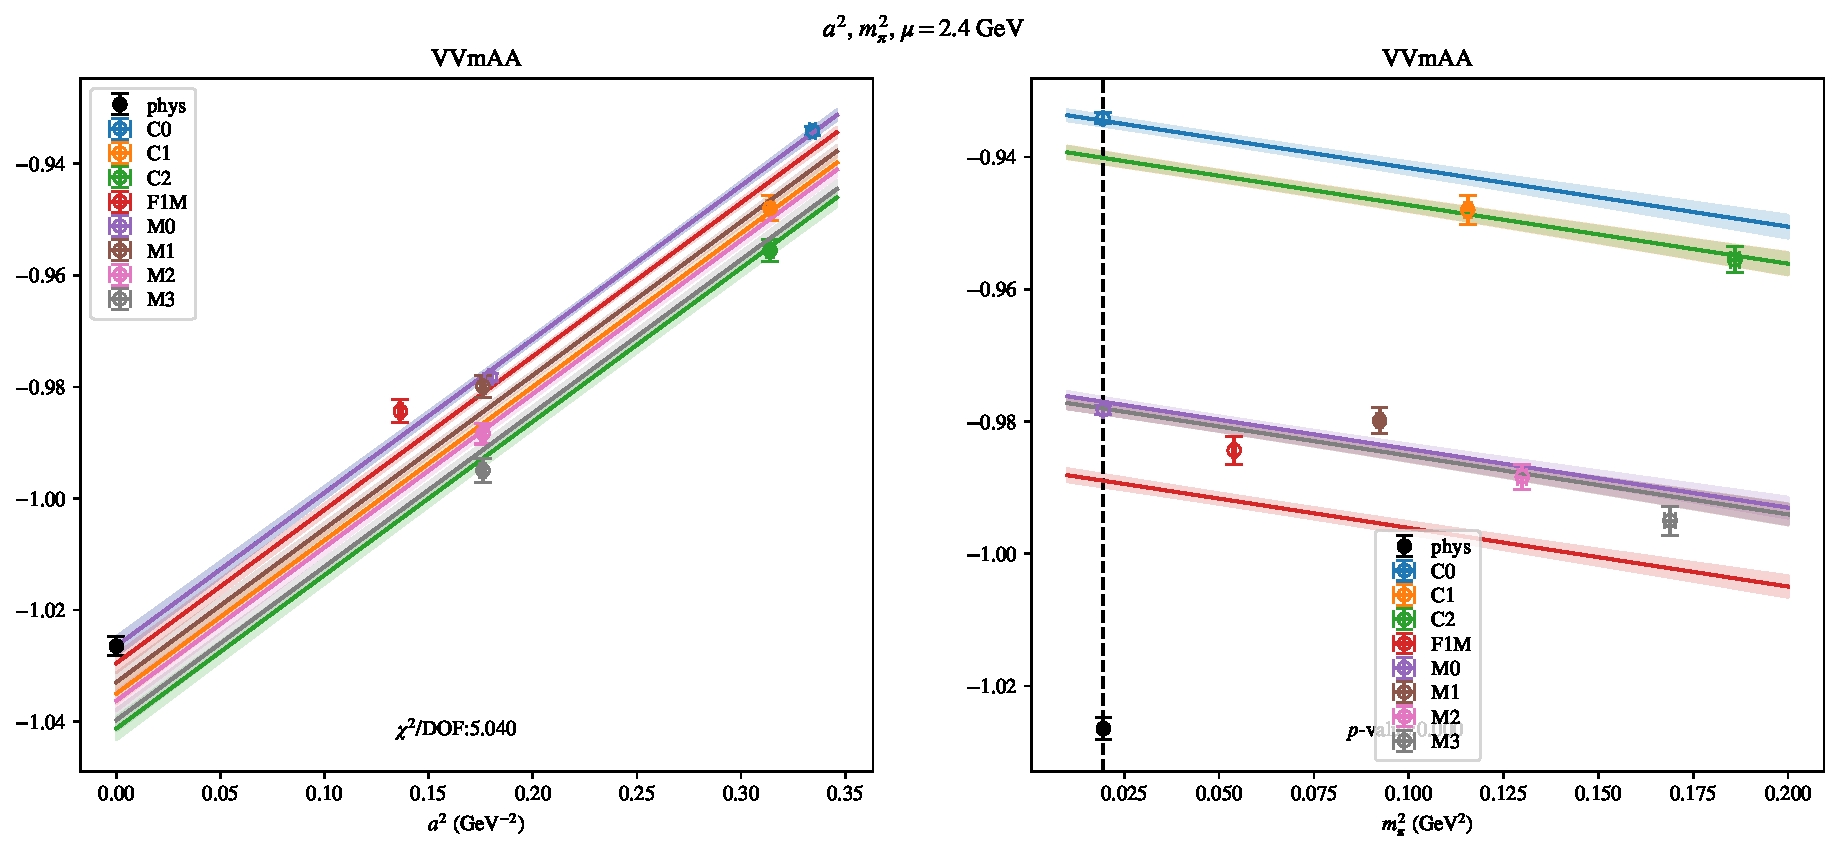
\includepdf[link, pages=-]{VVmAA/NPR/a2m2_24.pdf}
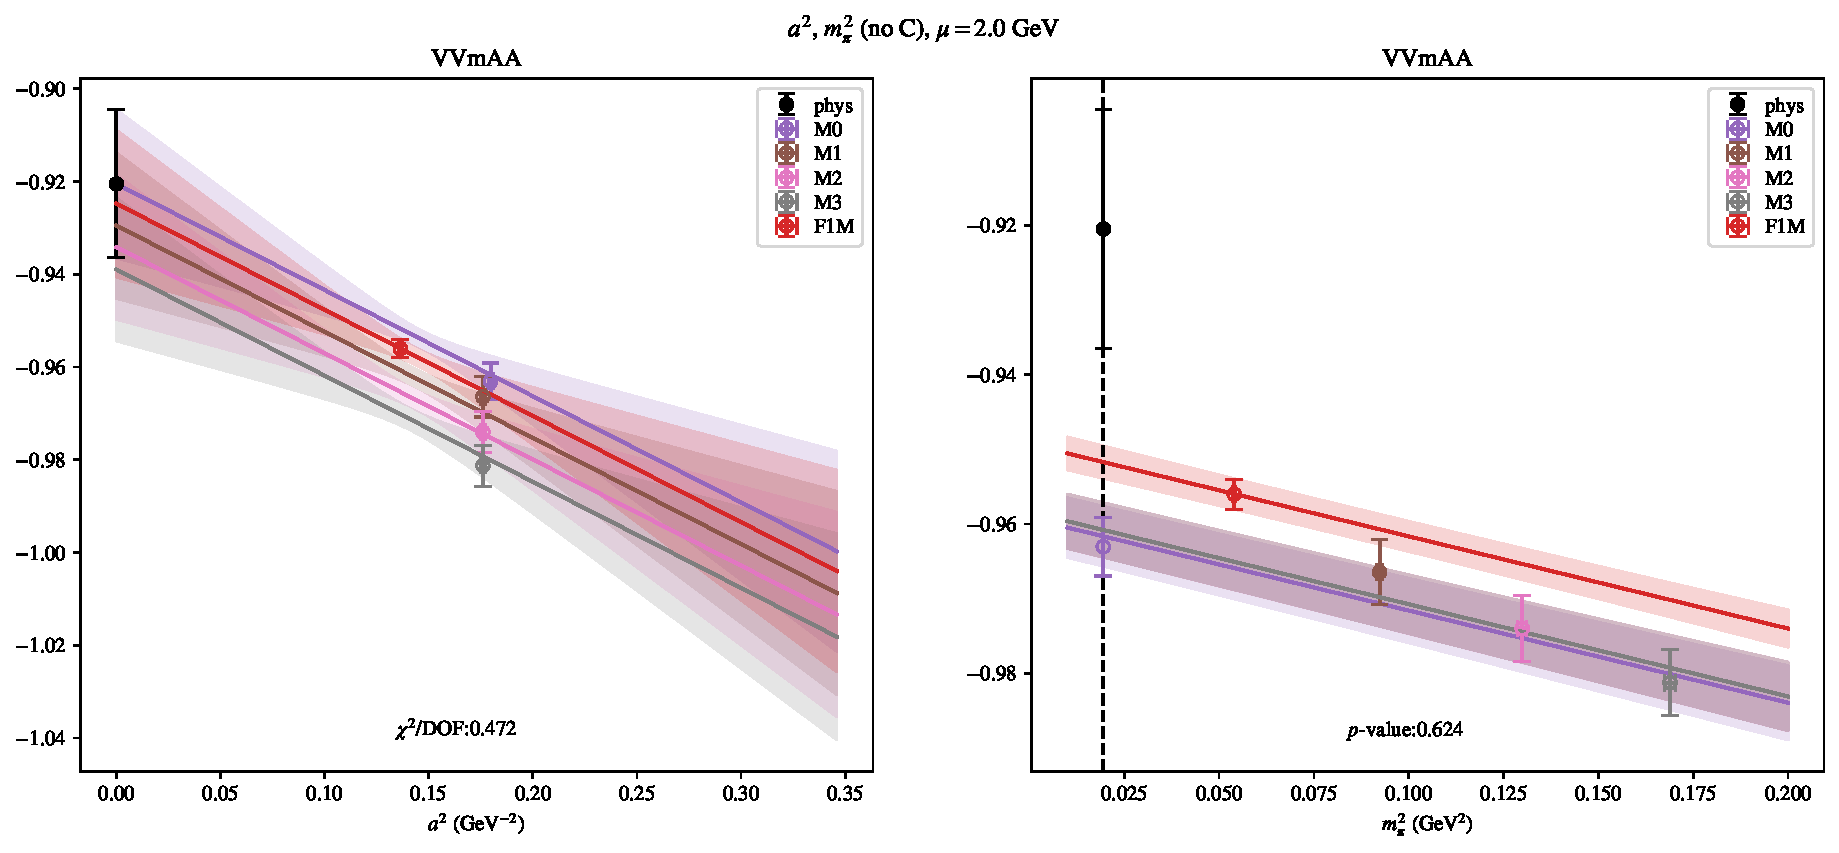
\includepdf[link, pages=-]{VVmAA/NPR/a2m2noC_20.pdf}
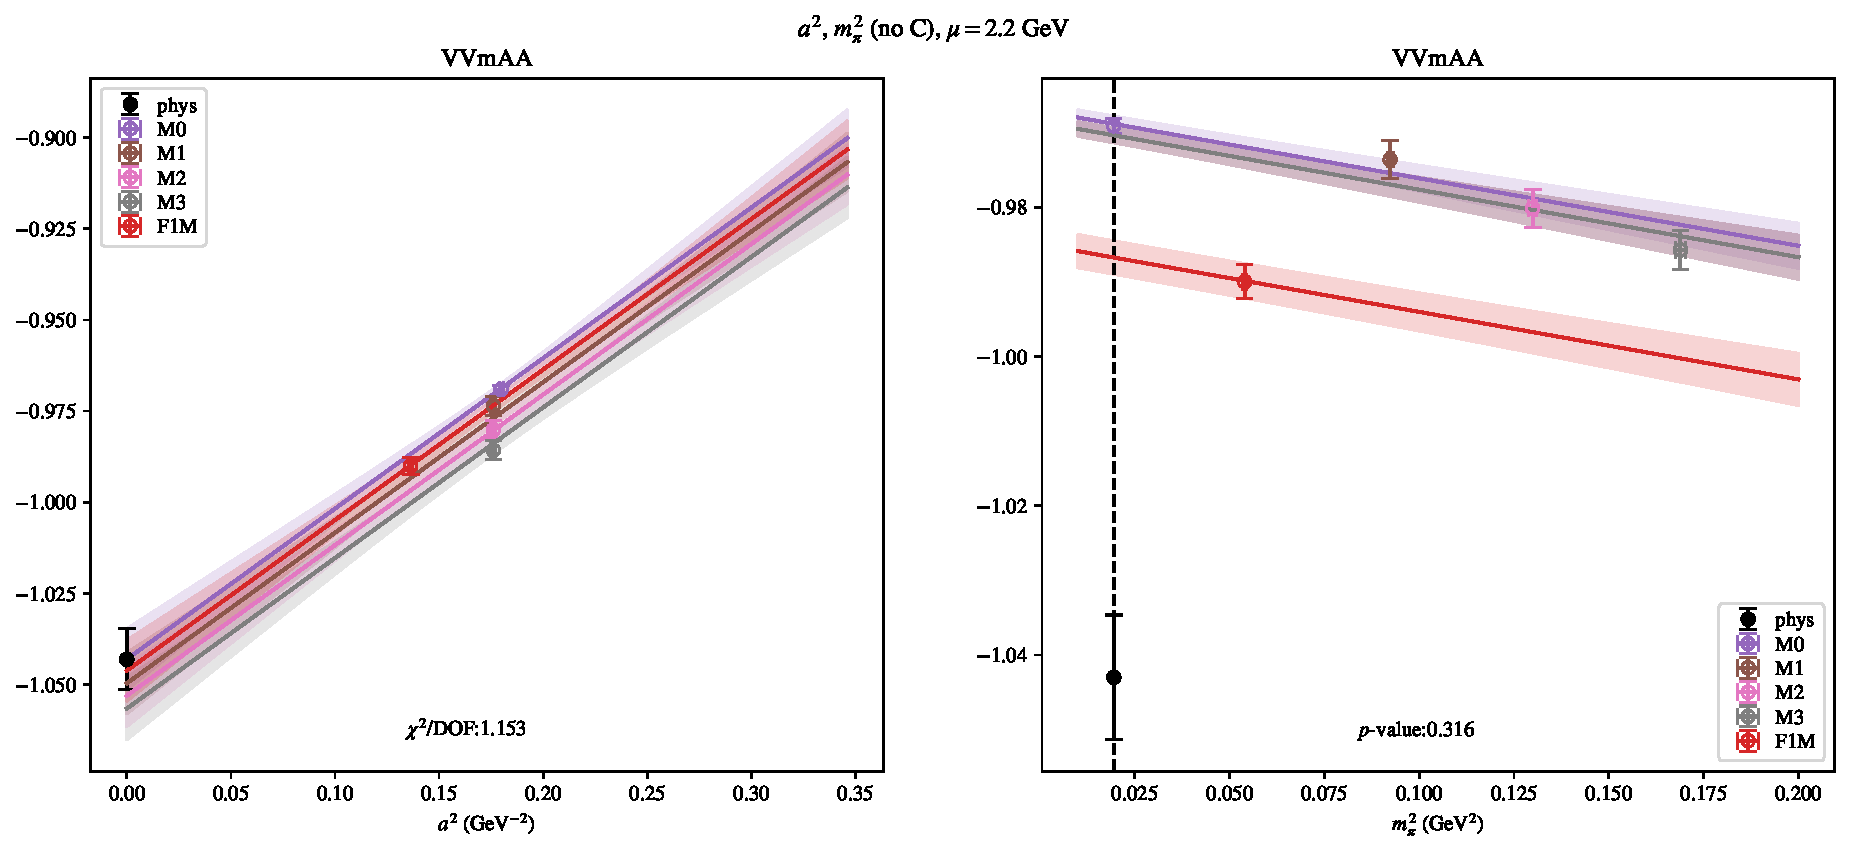
\includepdf[link, pages=-]{VVmAA/NPR/a2m2noC_22.pdf}
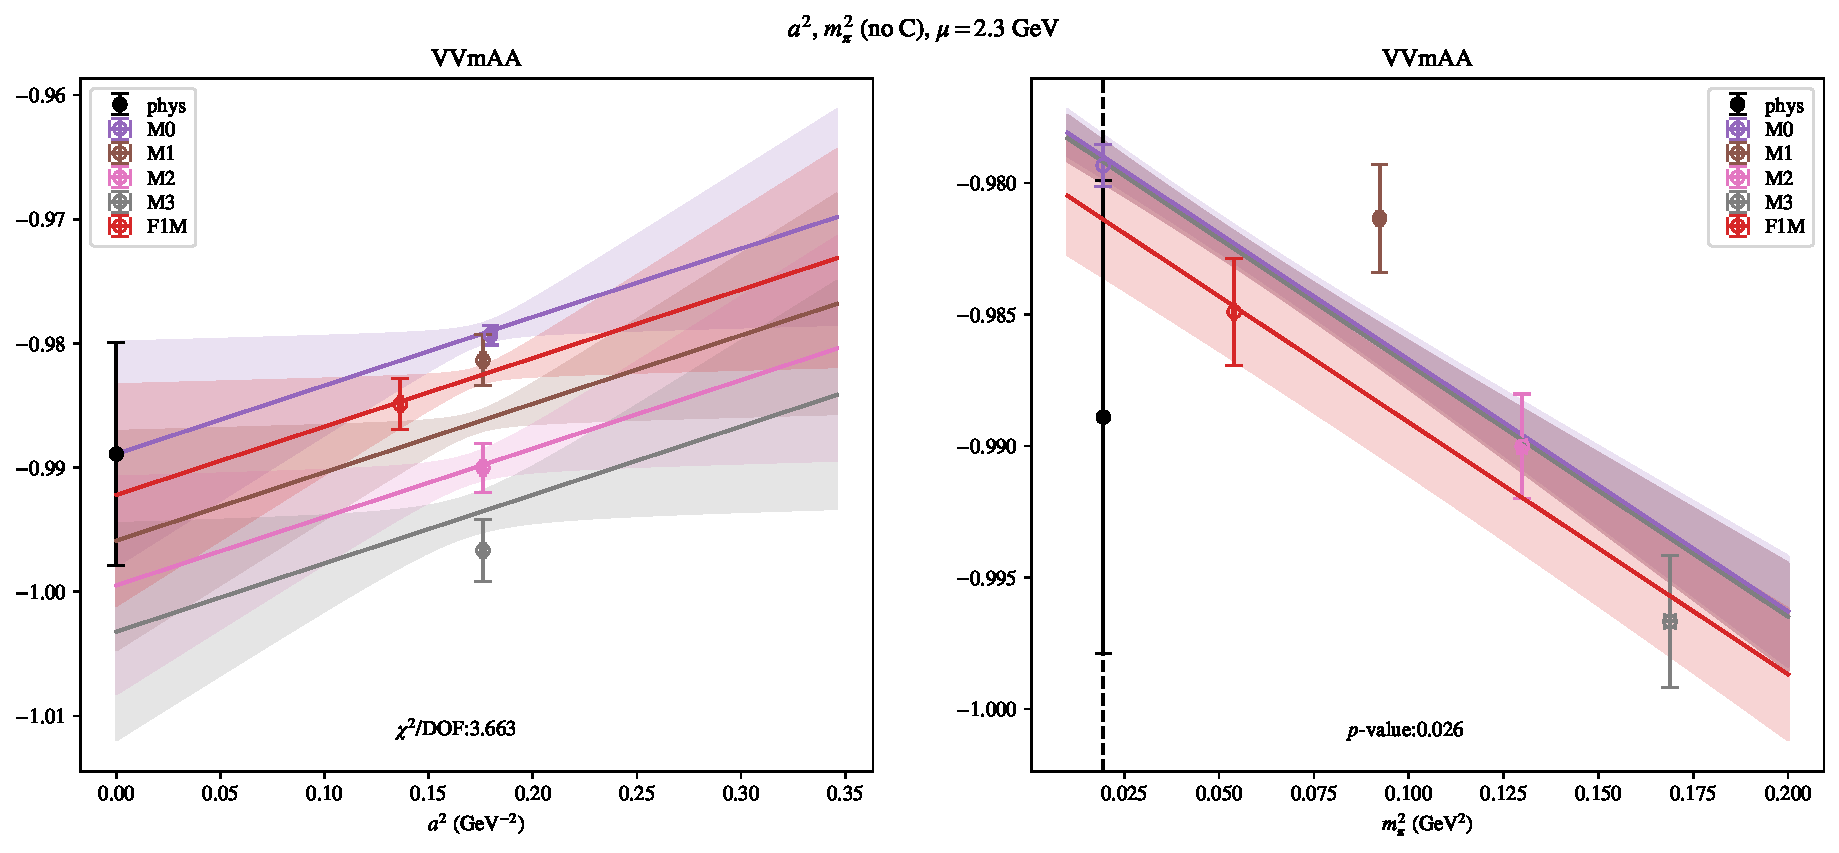
\includepdf[link, pages=-]{VVmAA/NPR/a2m2noC_23.pdf}
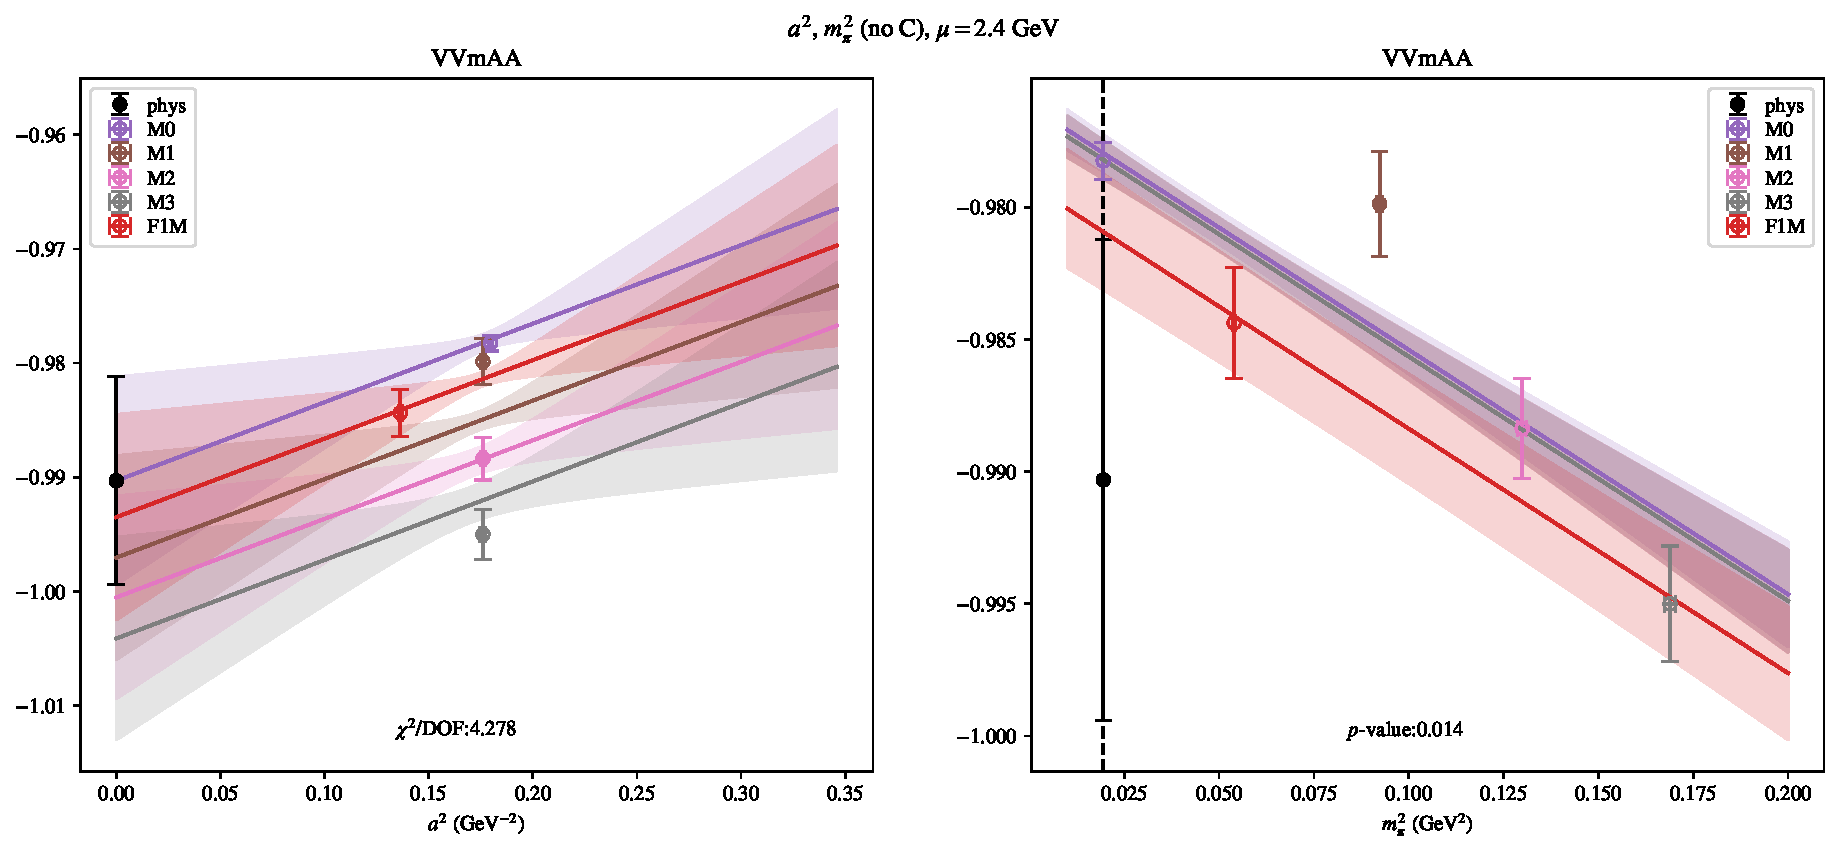
\includepdf[link, pages=-]{VVmAA/NPR/a2m2noC_24.pdf}
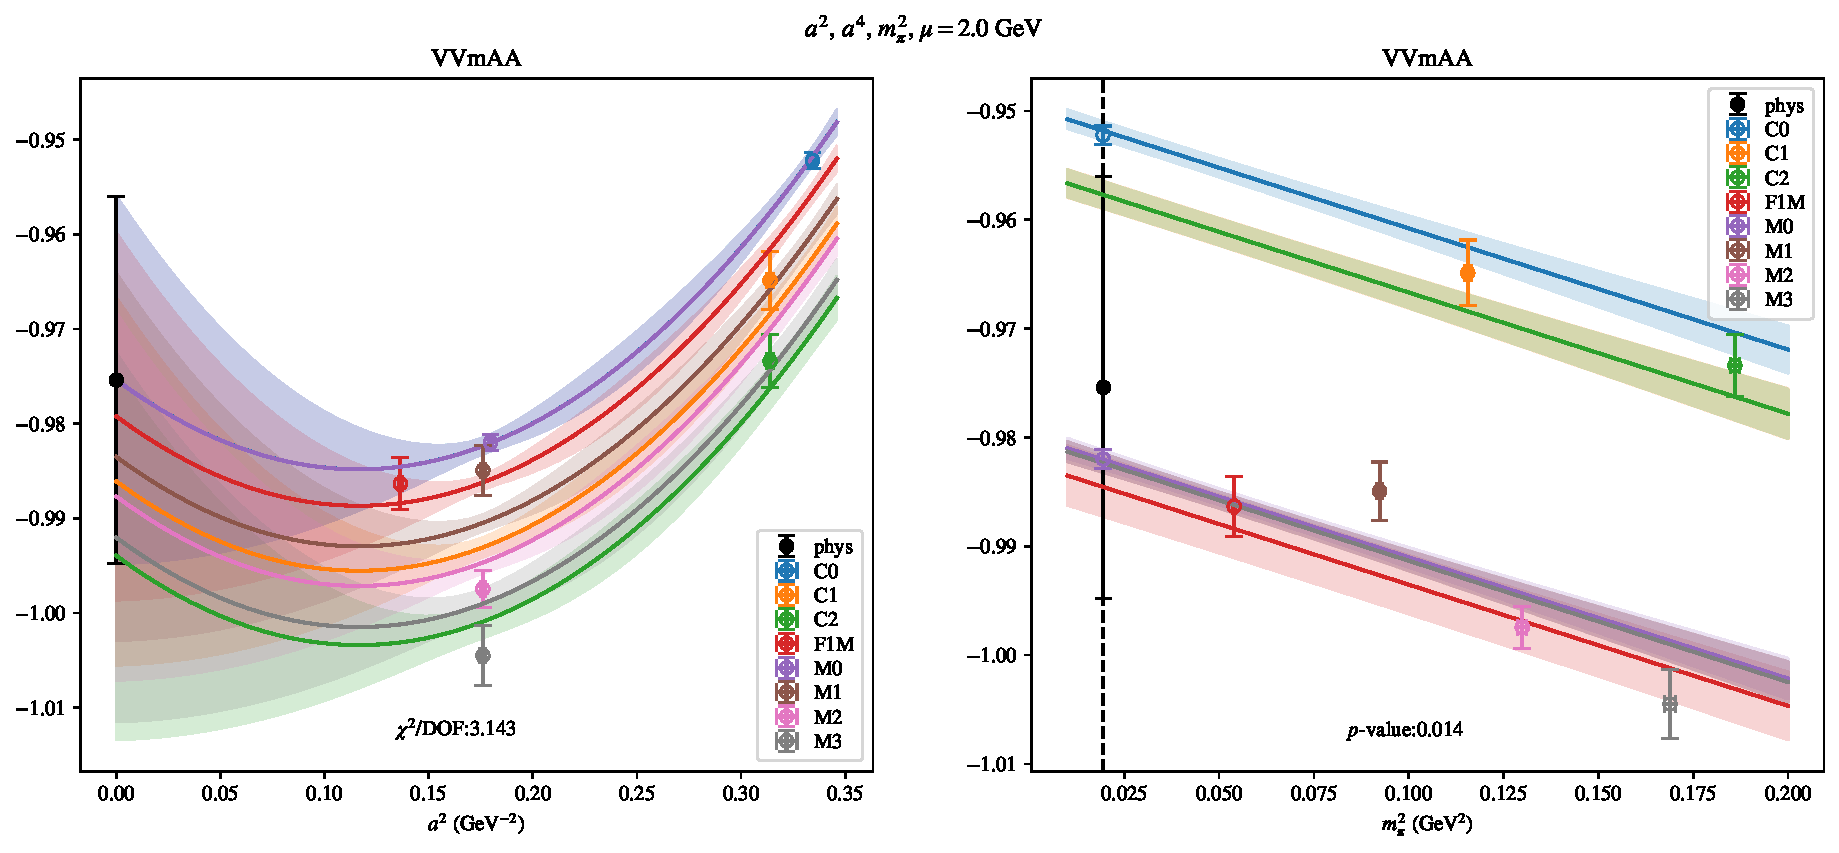
\includepdf[link, pages=-]{VVmAA/NPR/a2a4m2_20.pdf}
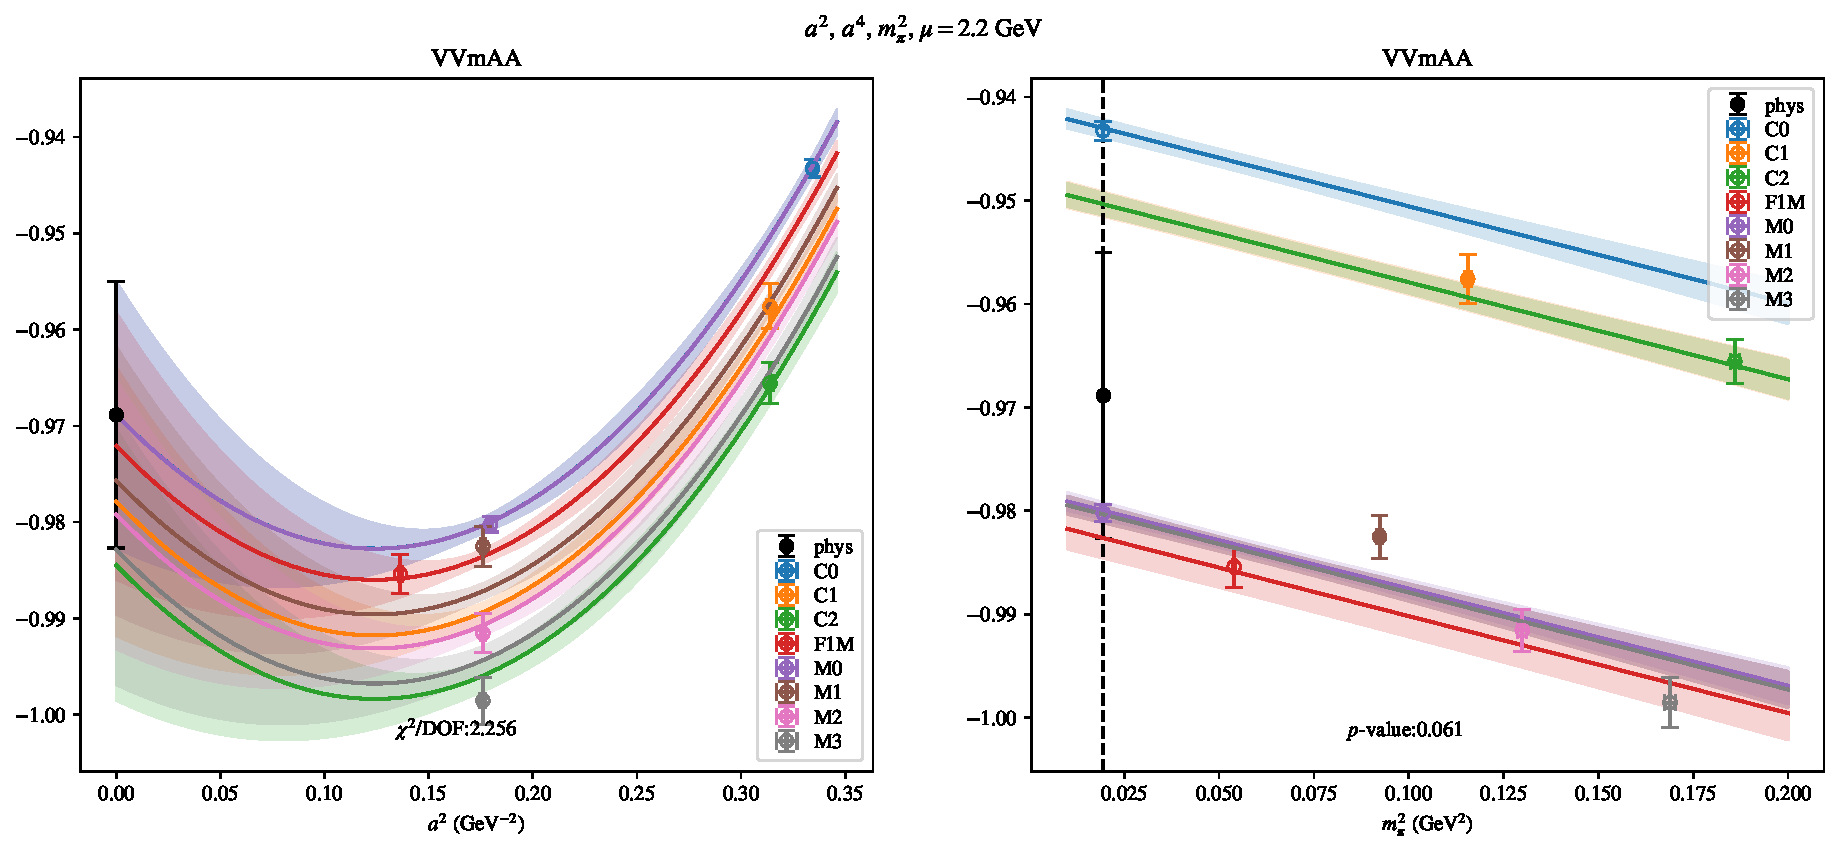
\includepdf[link, pages=-]{VVmAA/NPR/a2a4m2_22.pdf}
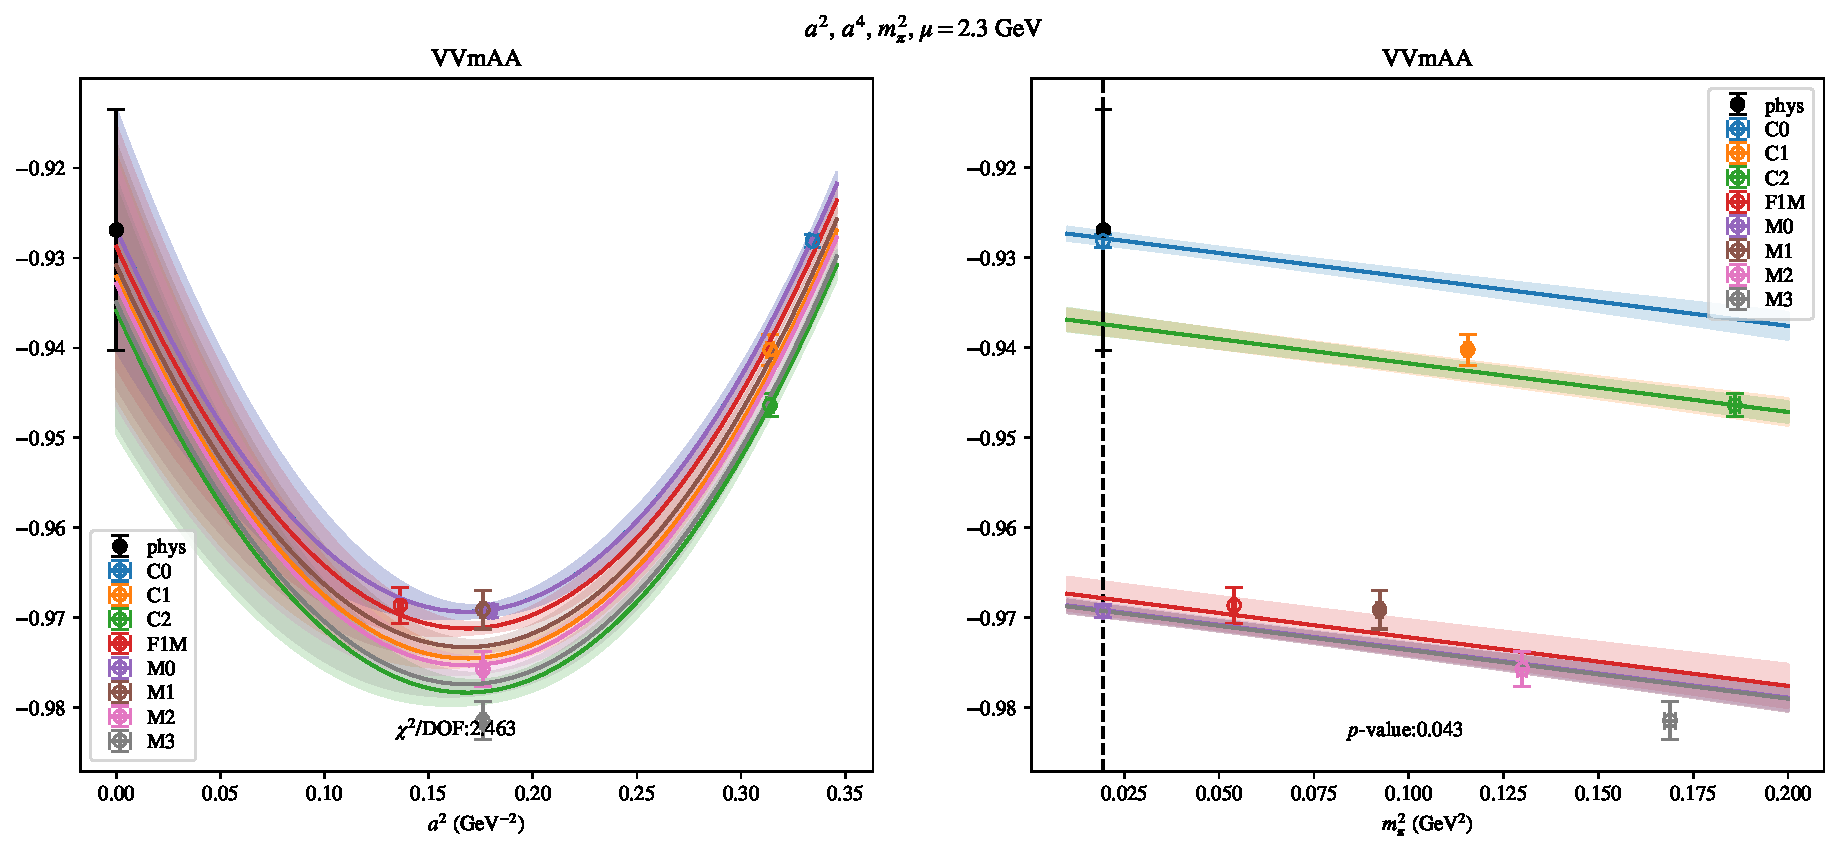
\includepdf[link, pages=-]{VVmAA/NPR/a2a4m2_23.pdf}
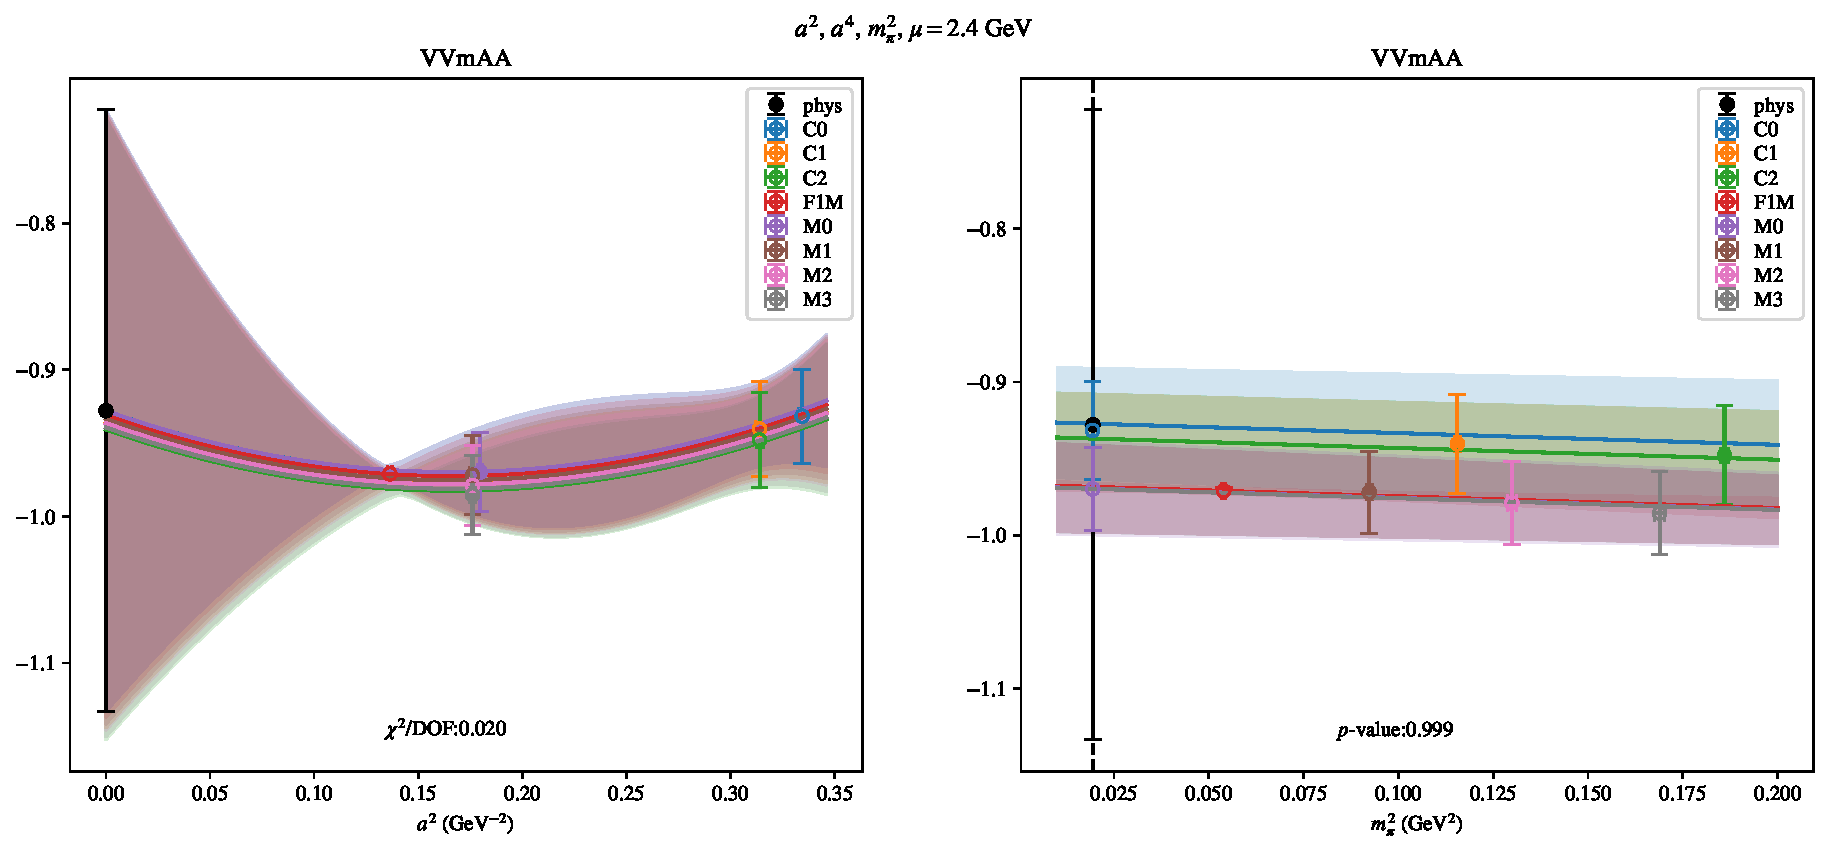
\includepdf[link, pages=-]{VVmAA/NPR/a2a4m2_24.pdf}
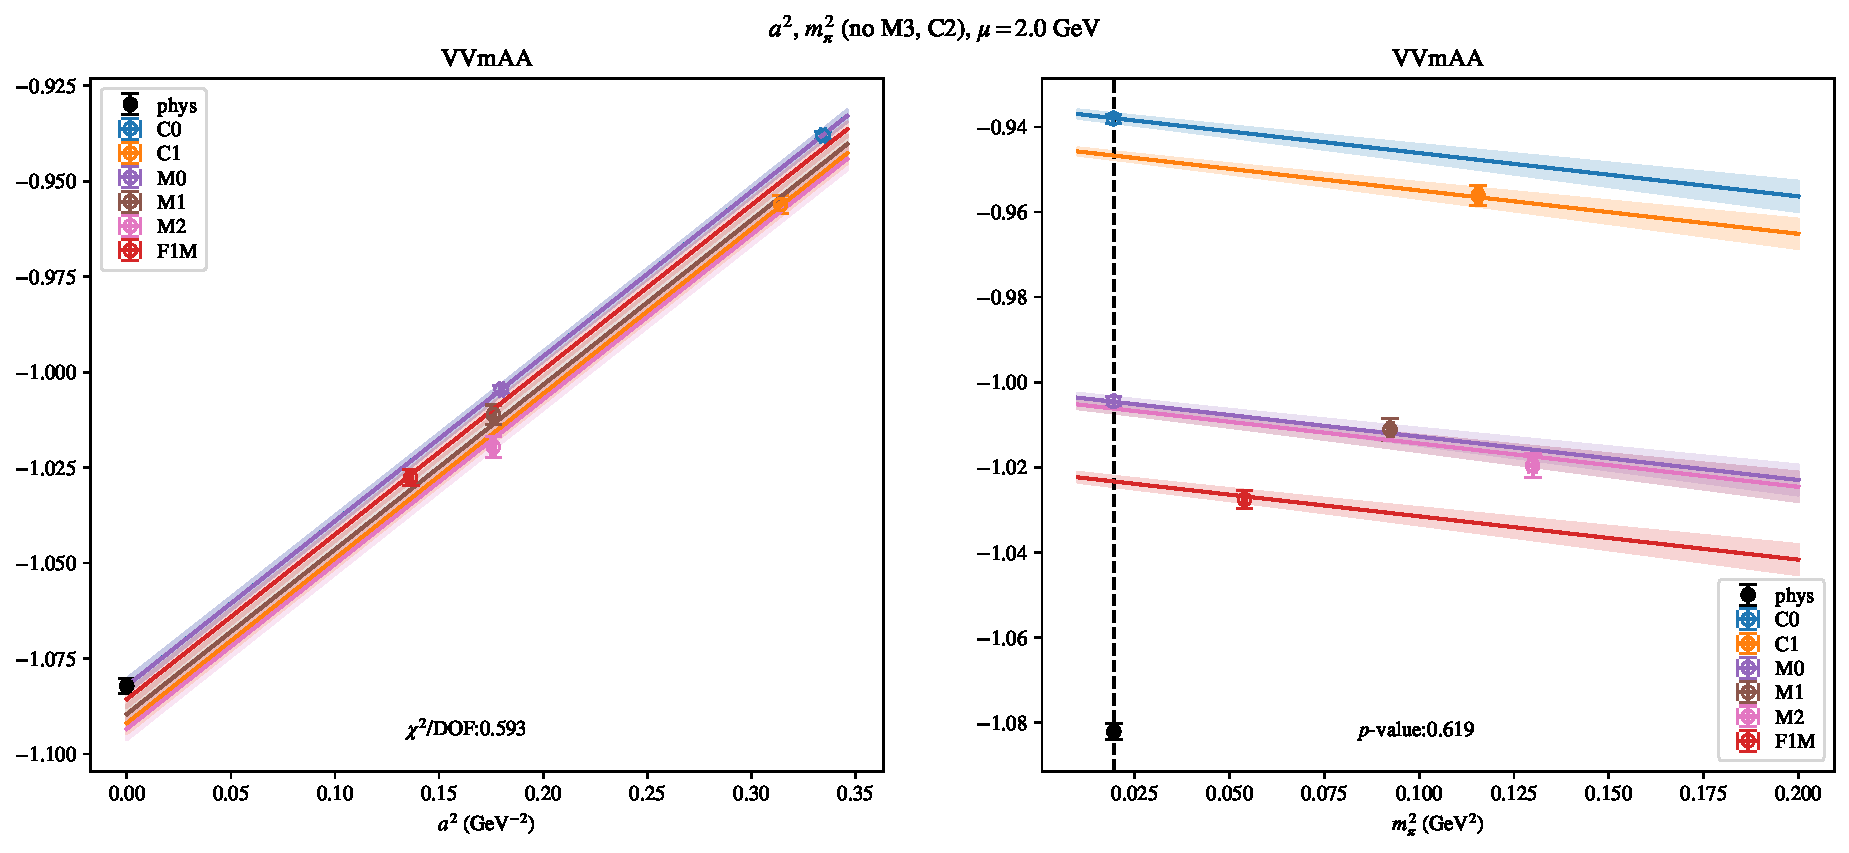
\includepdf[link, pages=-]{VVmAA/NPR/a2m2mcut_20.pdf}
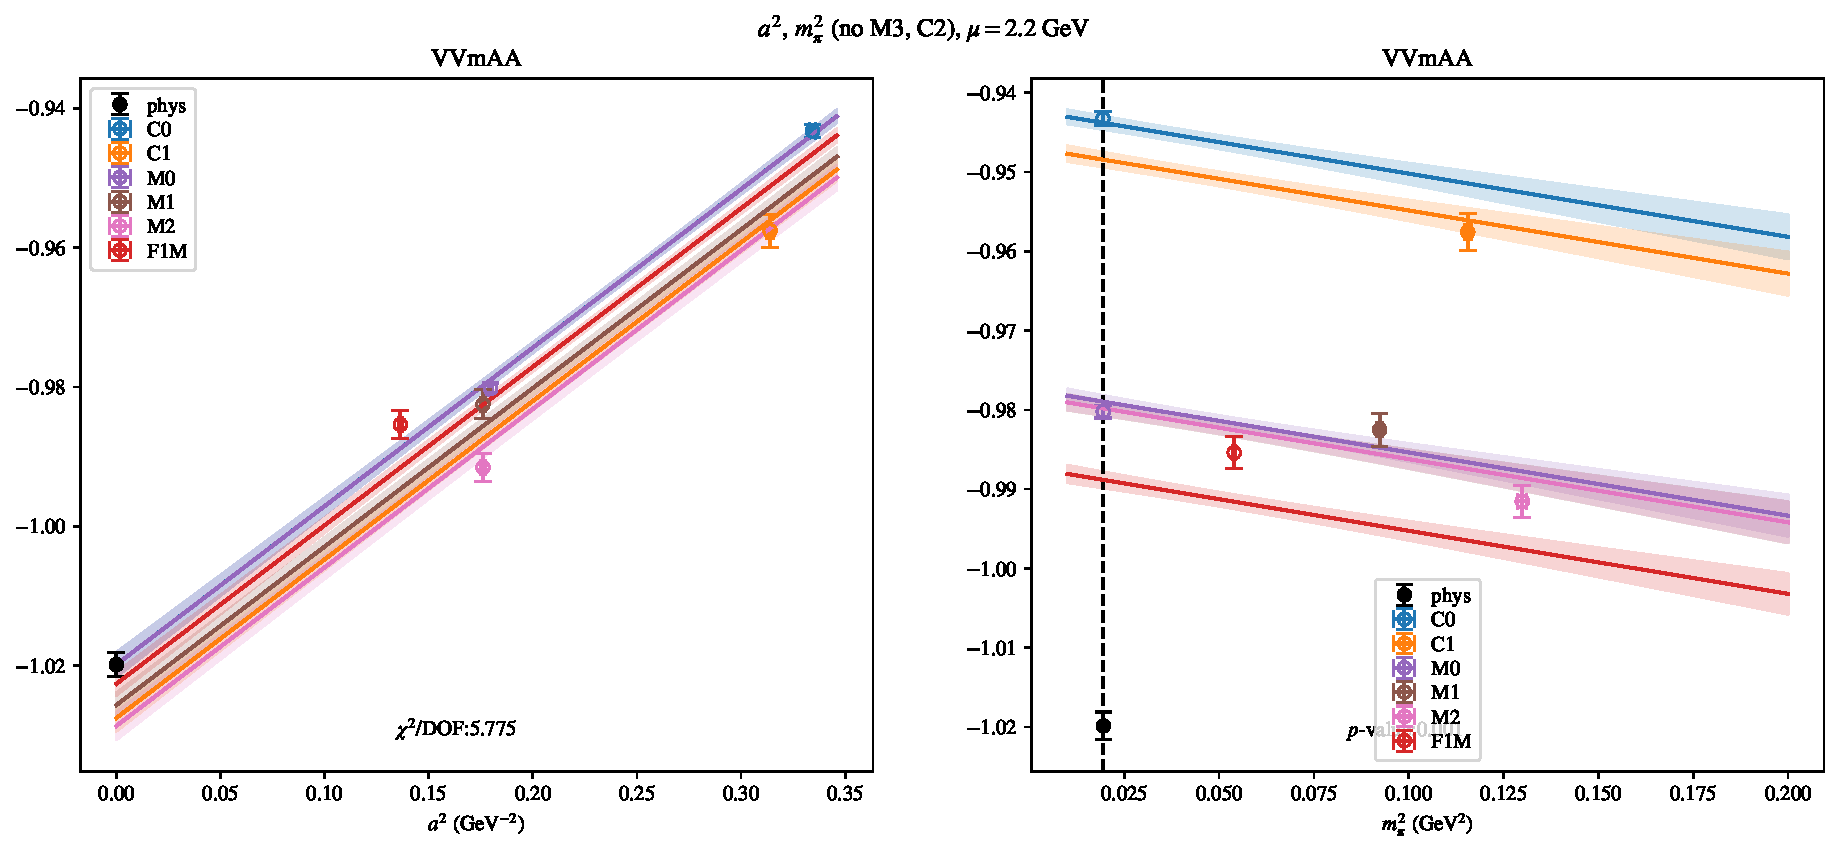
\includepdf[link, pages=-]{VVmAA/NPR/a2m2mcut_22.pdf}
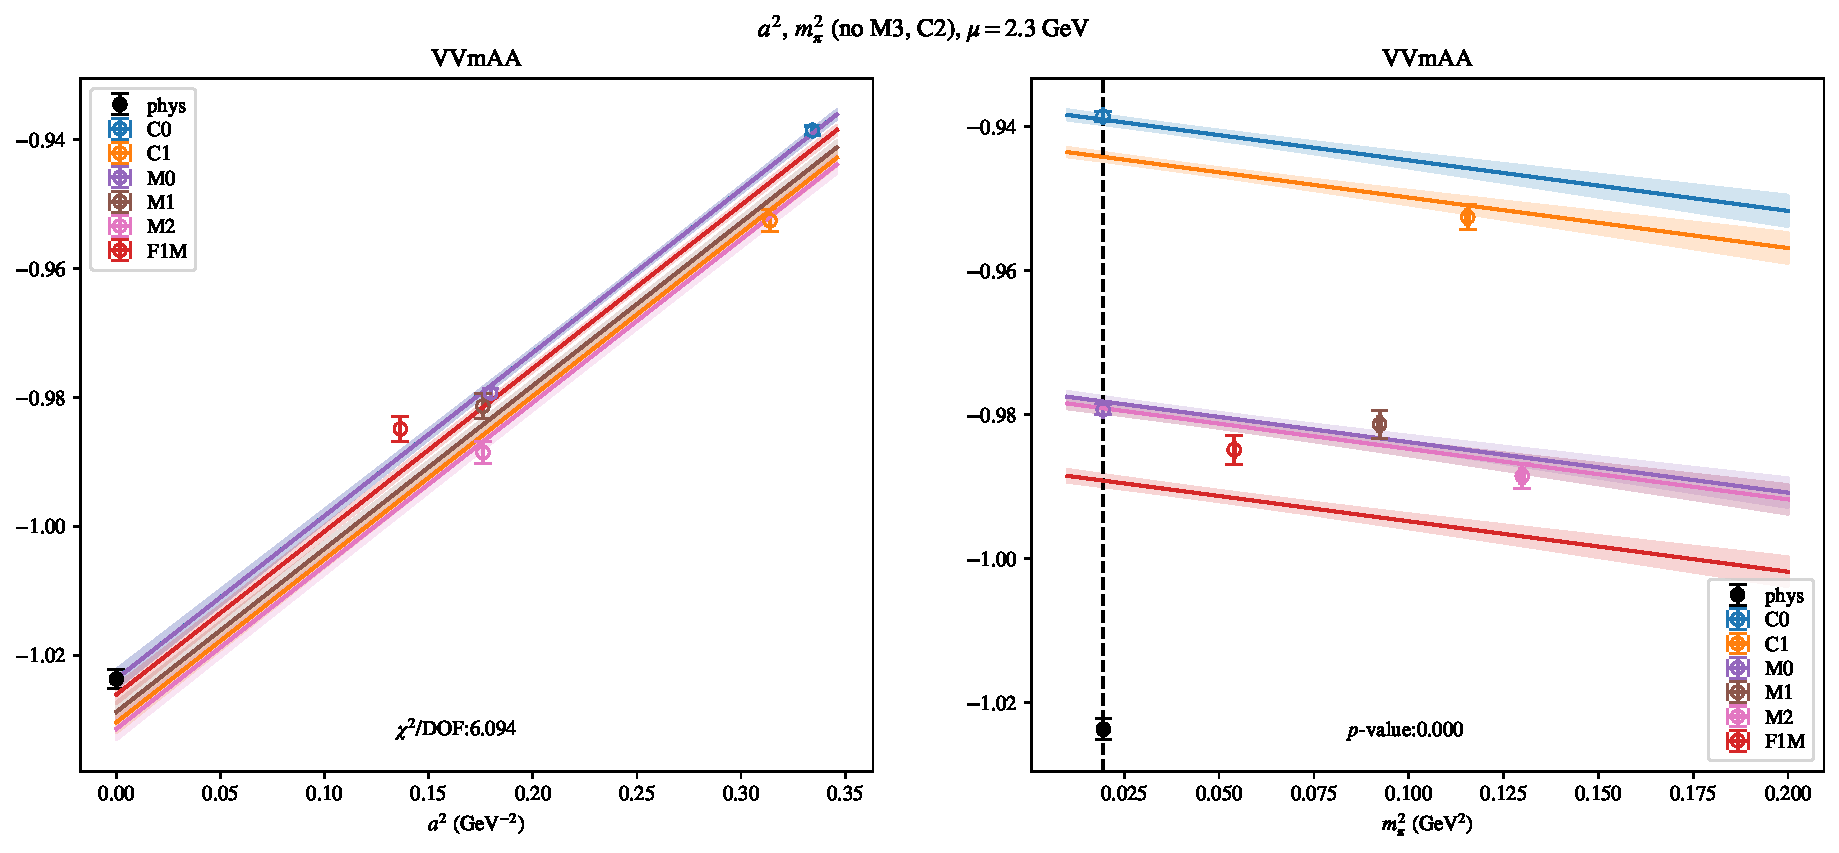
\includepdf[link, pages=-]{VVmAA/NPR/a2m2mcut_23.pdf}
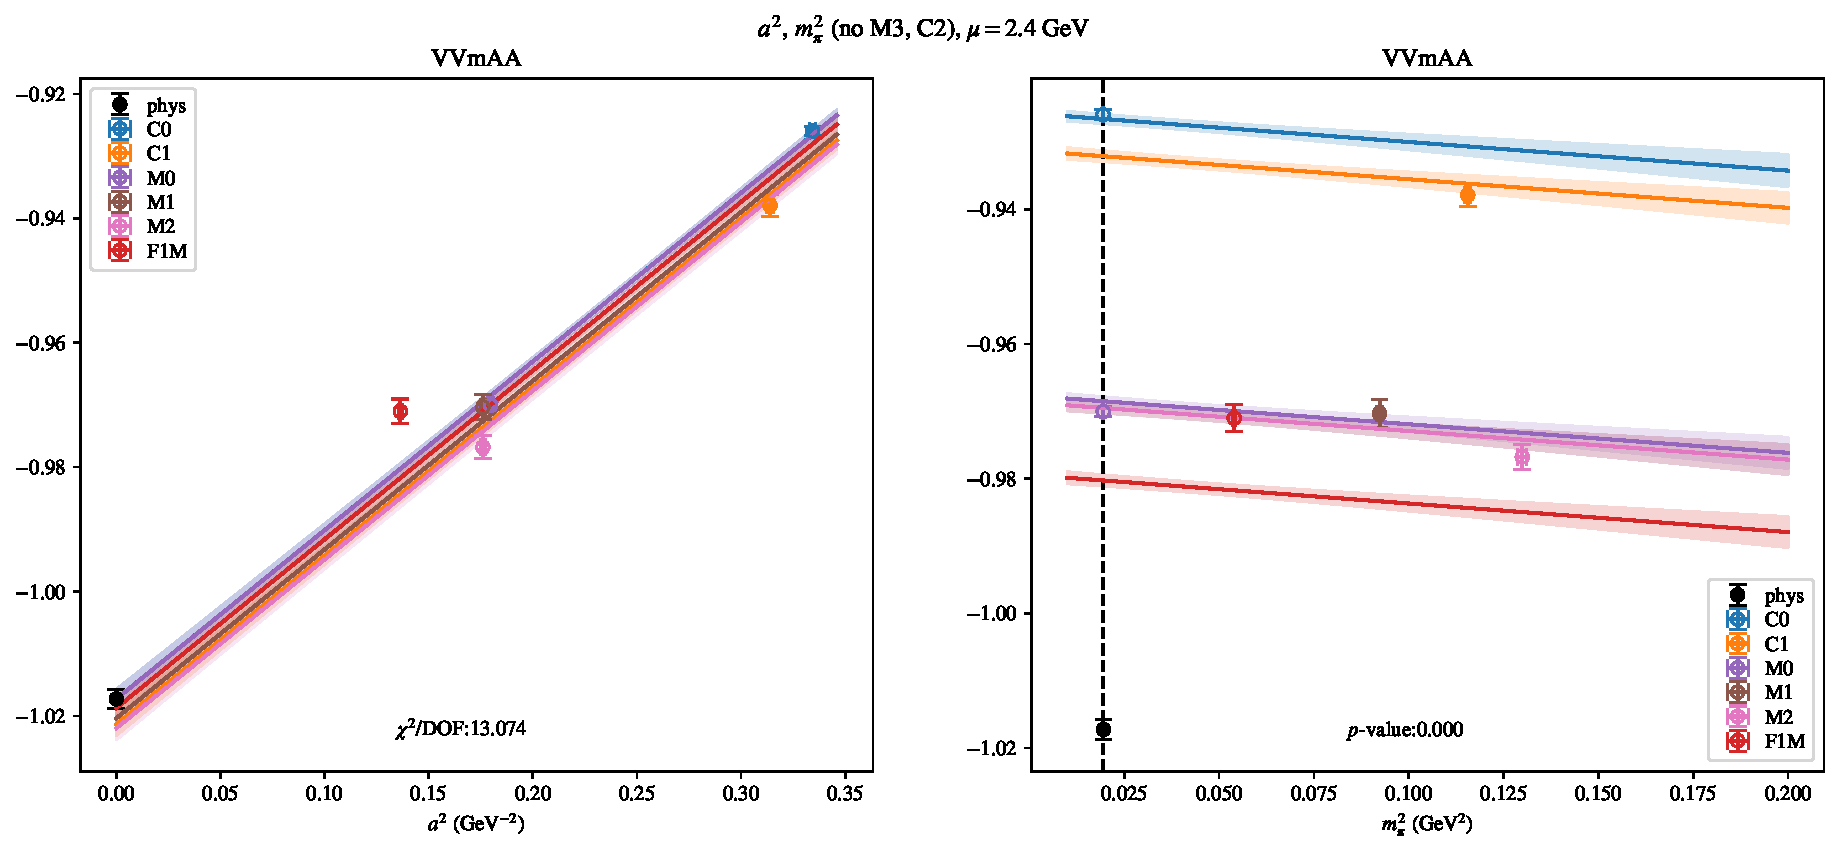
\includepdf[link, pages=-]{VVmAA/NPR/a2m2mcut_24.pdf}
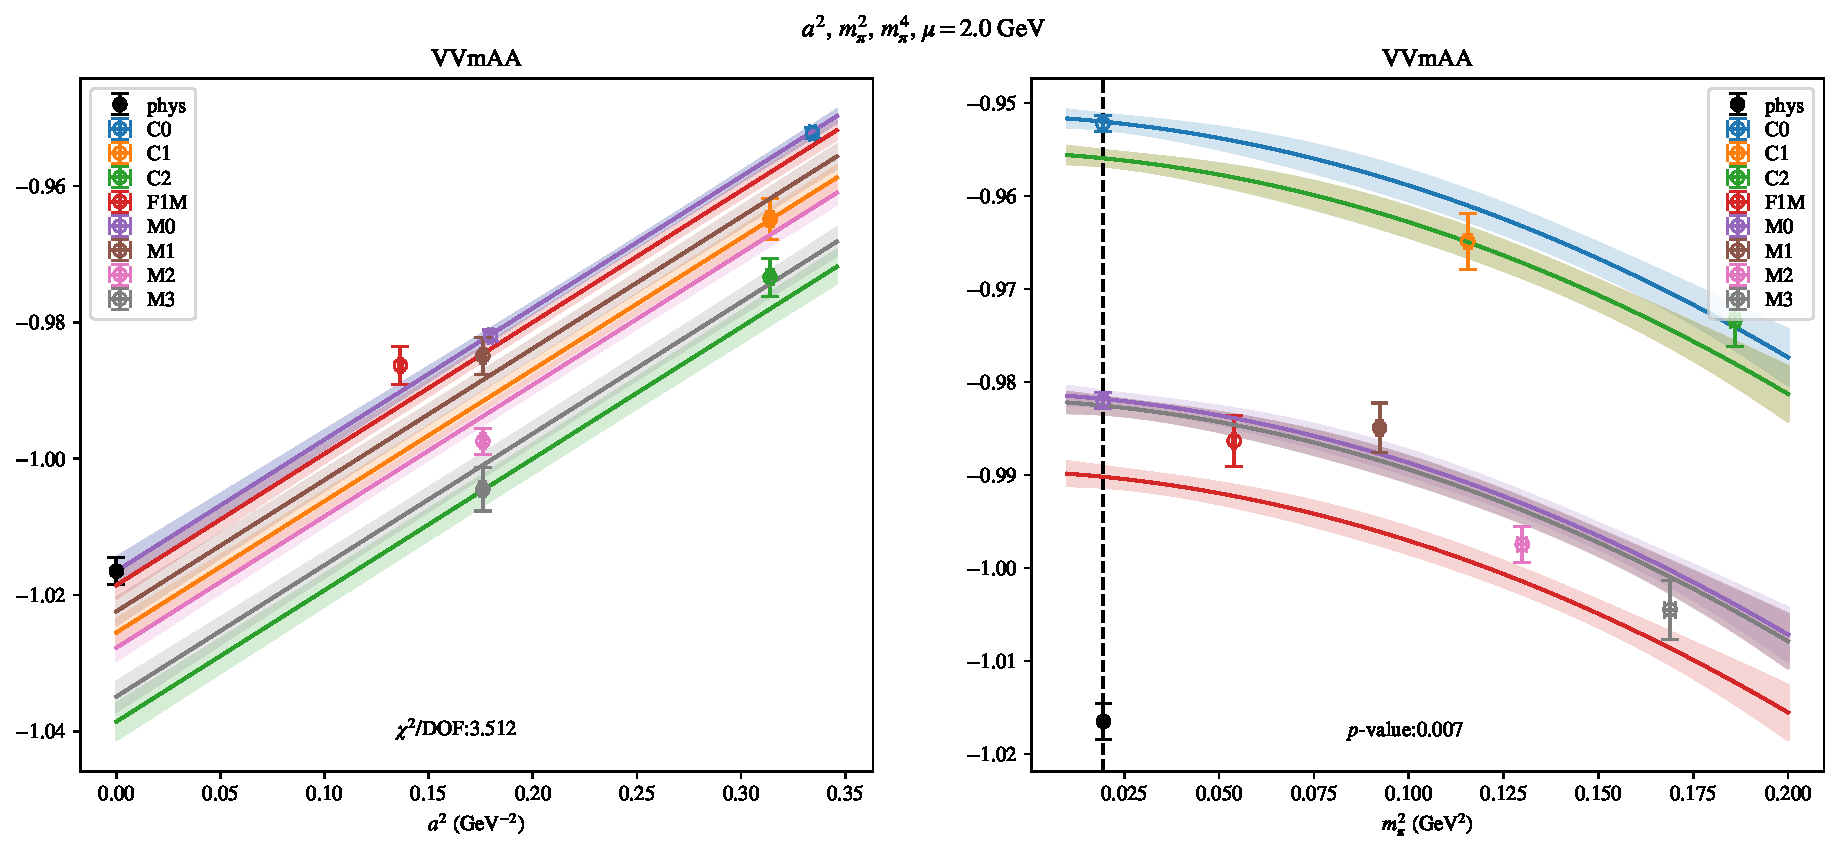
\includepdf[link, pages=-]{VVmAA/NPR/a2m2m4_20.pdf}
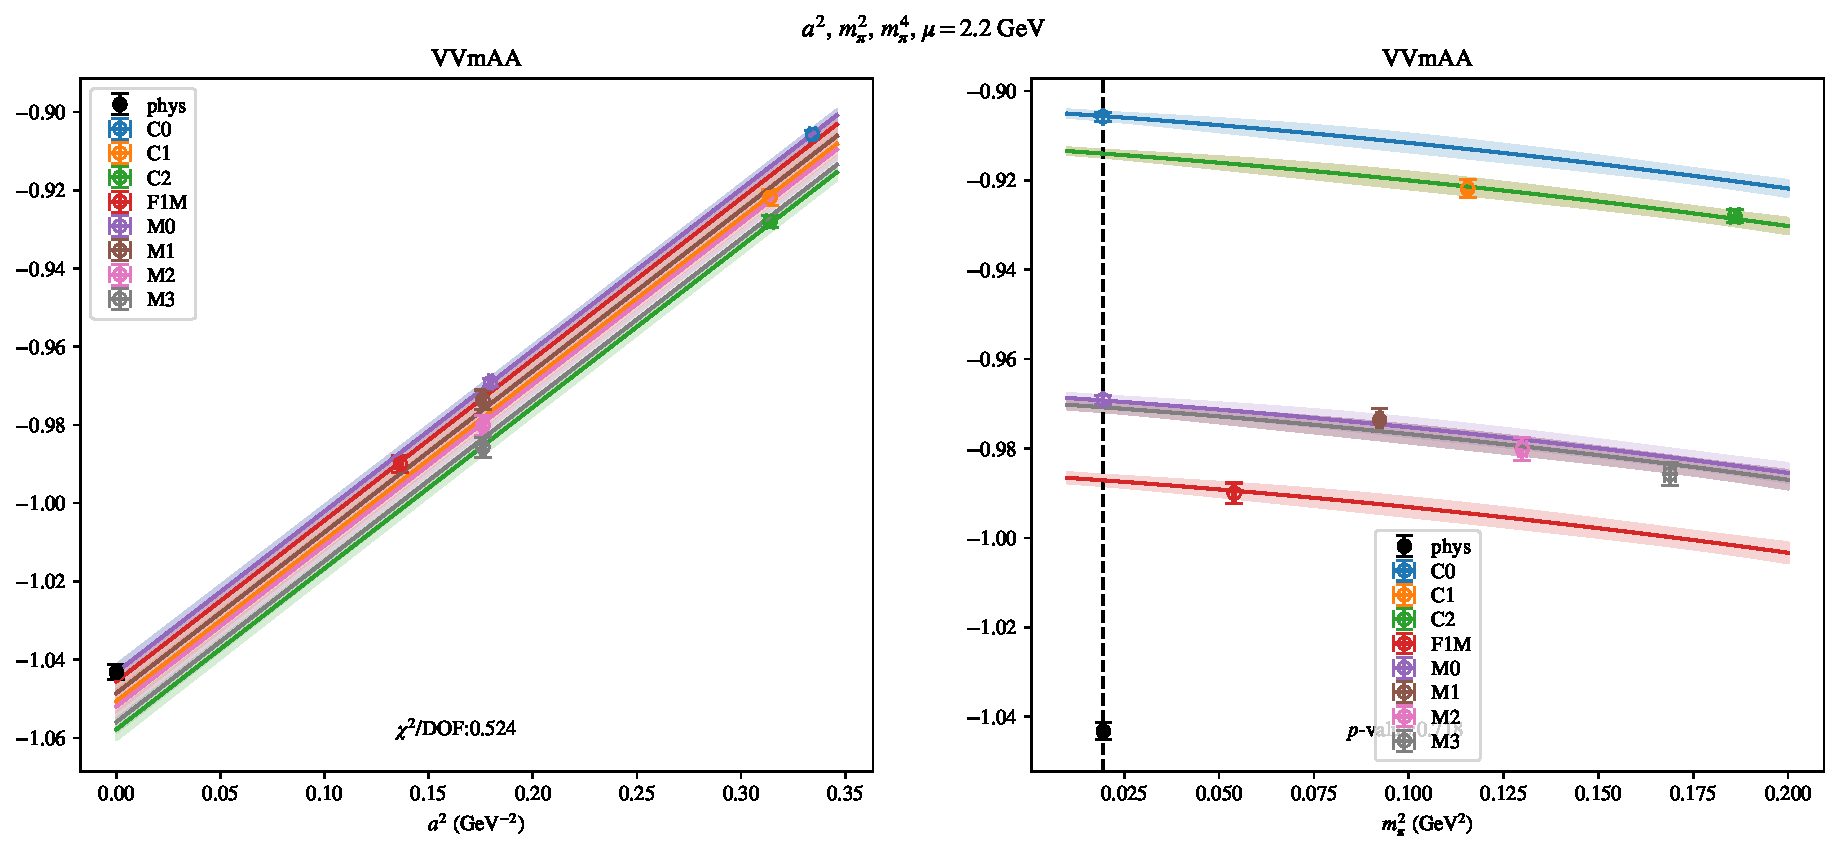
\includepdf[link, pages=-]{VVmAA/NPR/a2m2m4_22.pdf}
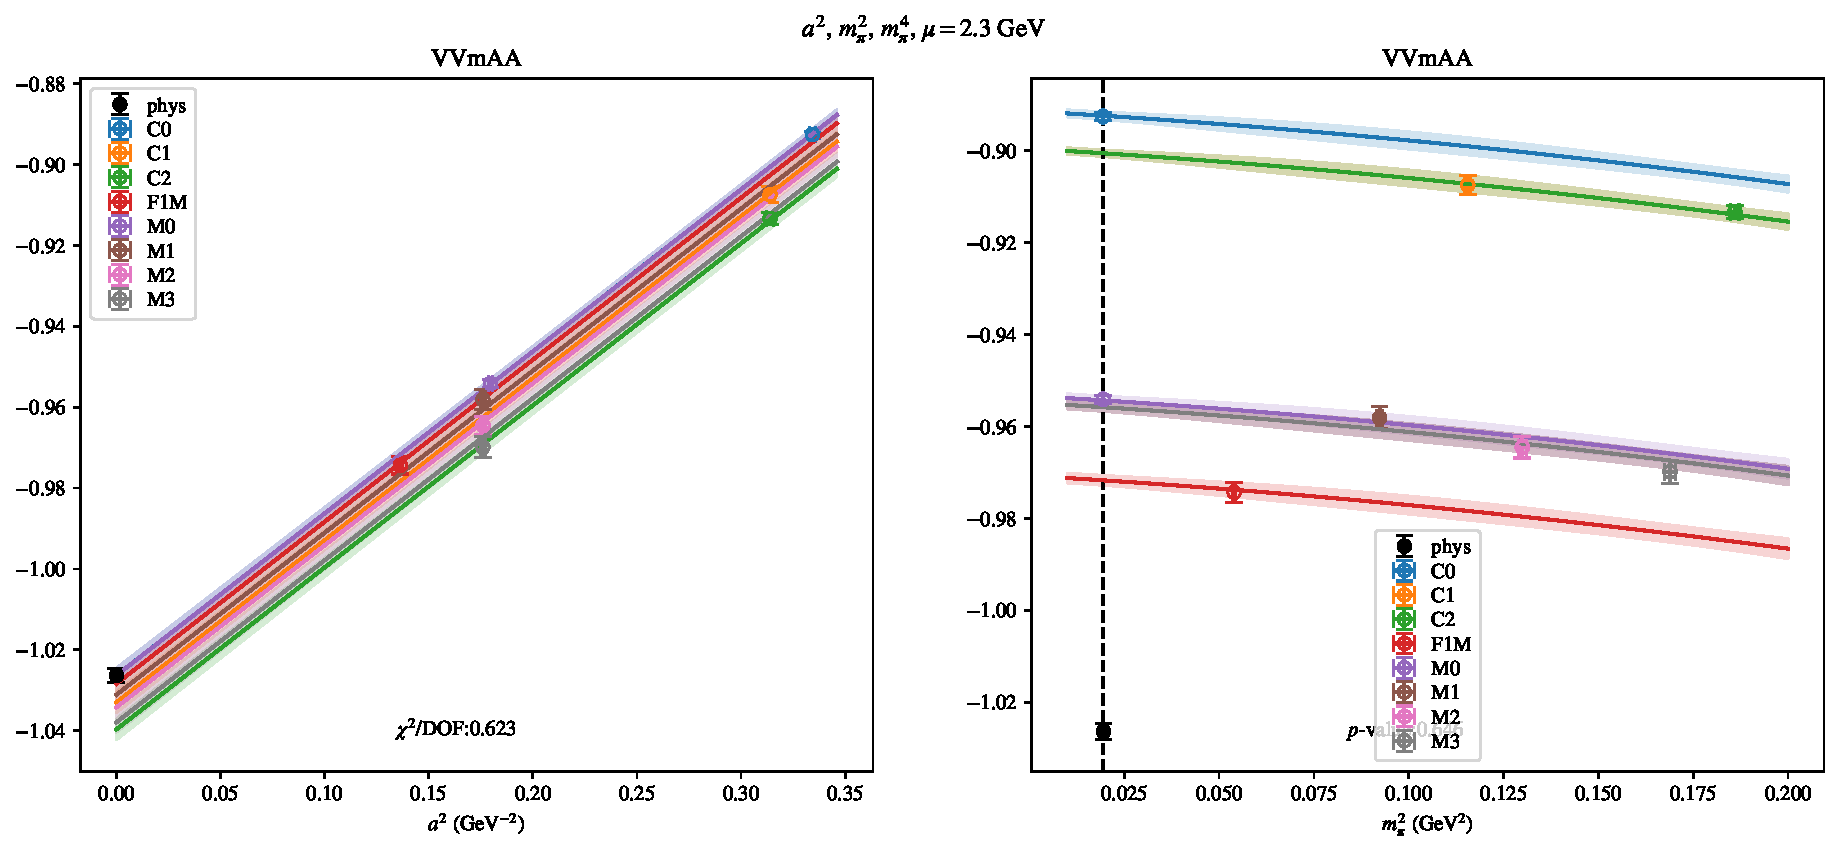
\includepdf[link, pages=-]{VVmAA/NPR/a2m2m4_23.pdf}
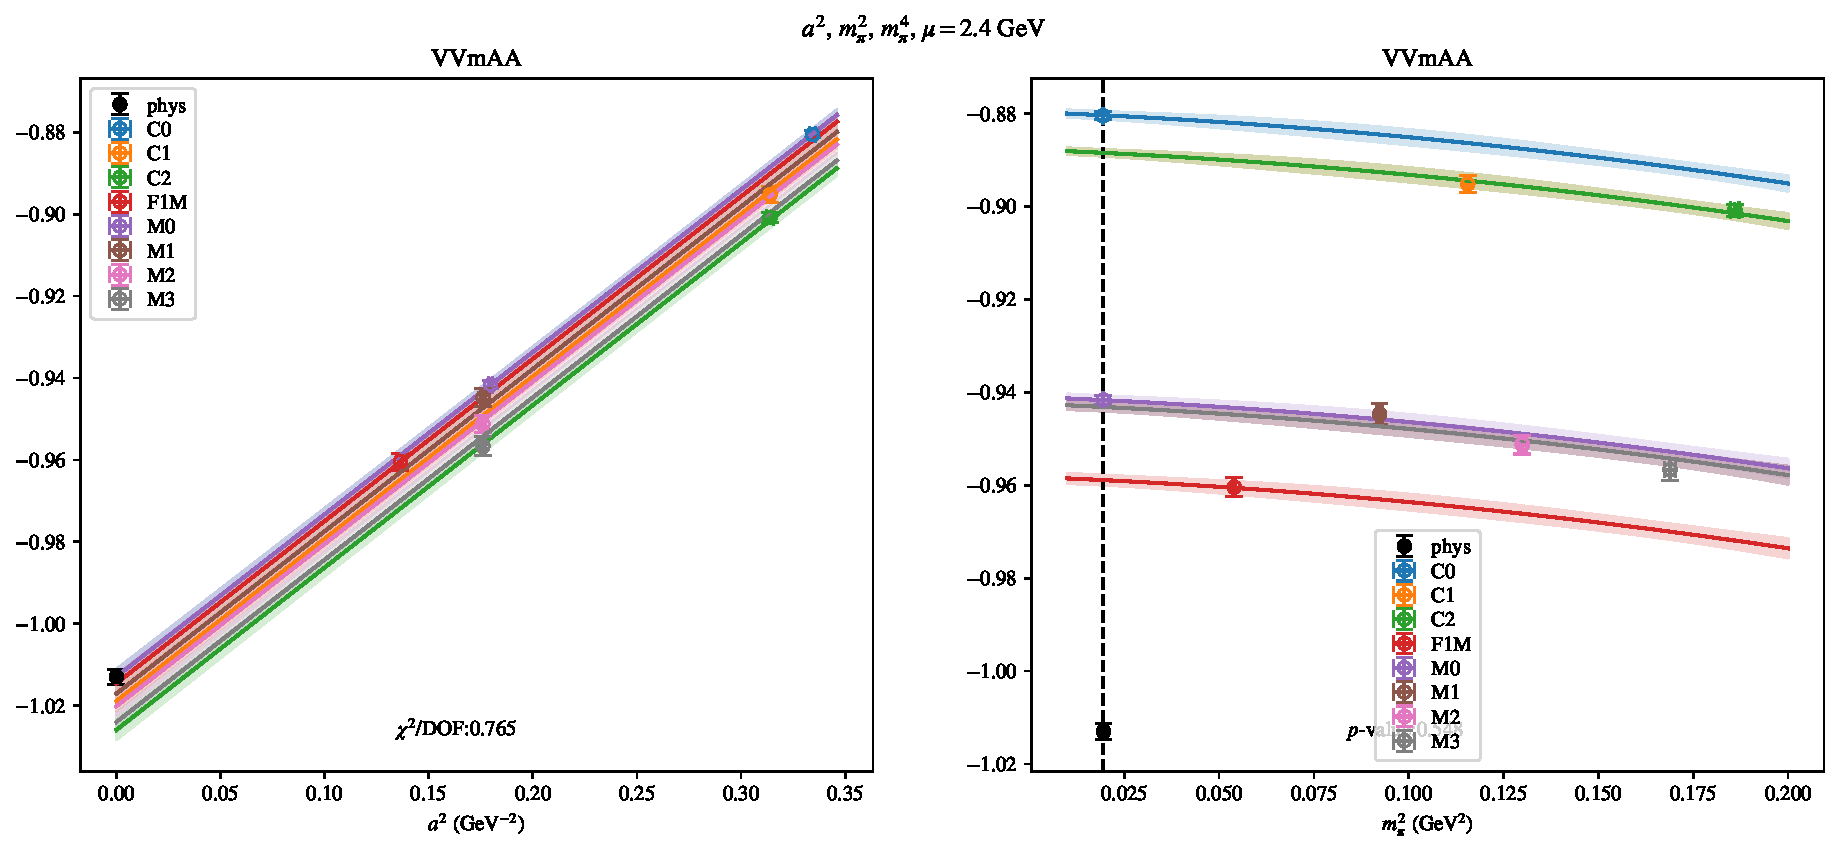
\includepdf[link, pages=-]{VVmAA/NPR/a2m2m4_24.pdf}
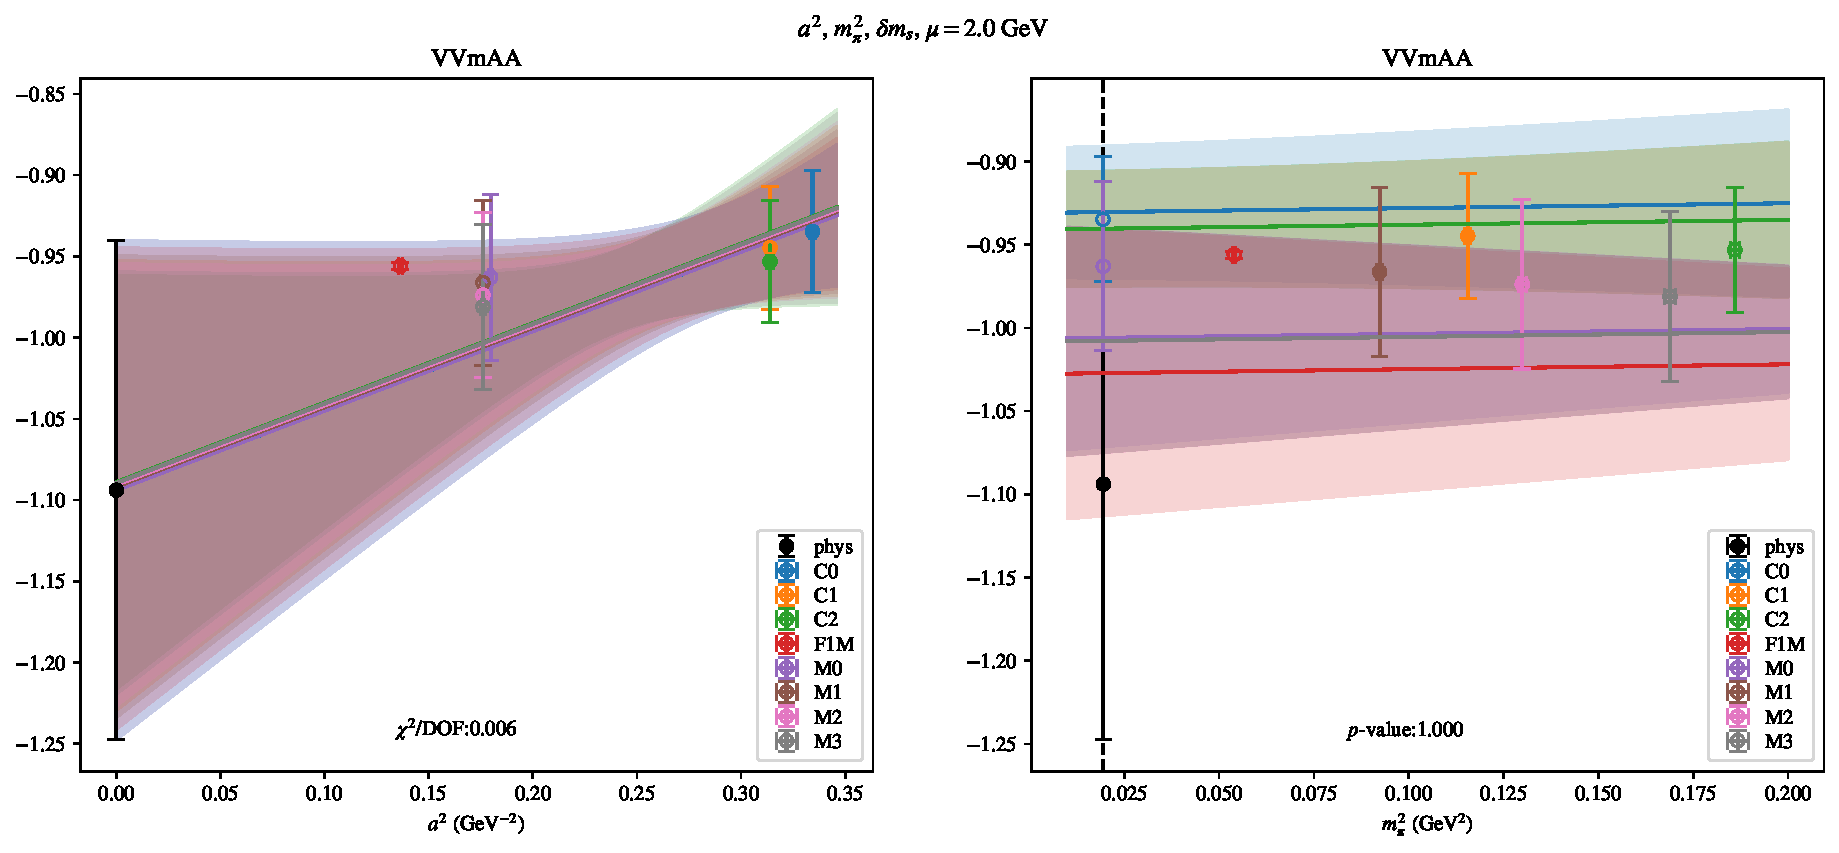
\includepdf[link, pages=-]{VVmAA/NPR/a2m2delm_20.pdf}
\includepdf[link, pages=-]{VVmAA/NPR/a2m2delm_22.pdf}
\includepdf[link, pages=-]{VVmAA/NPR/a2m2delm_23.pdf}
\includepdf[link, pages=-]{VVmAA/NPR/a2m2delm_24.pdf}
\clearpage
\section{$\mathcal{B}_3$}
\begin{table}[h!]
\begin{center}
\begin{tabular}{|c|c|c|c|c|c|c|}
\hline
$\mu$ (GeV) & $a^2$, $m_\pi^2$& $a^2$, $m_\pi^2$ (no C)& $a^2$, $m_\pi^2$, $a^4$& $a^2$, $m_\pi^2$ (no M3, C2)& $a^2$, $m_\pi^2$, $m_\pi^4$& $a^2$, $m_\pi^2$, $\delta m_s$\\
\hline
2.0& \hyperlink{SSmPP/NPR/a2m2_20.pdf.1}{\textbf{1.8033(46)}: 19.086 (0.0)} & \hyperlink{SSmPP/NPR/a2m2noC_20.pdf.1}{\textbf{1.662(20)}: 0.13 (0.878)} & \hyperlink{SSmPP/NPR/a2a4m2_20.pdf.1}{\textbf{1.591(23)}: 1.086 (0.361)} & \hyperlink{SSmPP/NPR/a2m2mcut_20.pdf.1}{\textbf{1.8053(46)}: 27.805 (0.0)} & \hyperlink{SSmPP/NPR/a2m2m4_20.pdf.1}{\textbf{1.8116(51)}: 13.649 (0.0)} & \hyperlink{SSmPP/NPR/a2m2delm_20.pdf.1}{\textbf{1.8160(57)}: 0.309 (0.872)}\\
2.2& \hyperlink{SSmPP/NPR/a2m2_22.pdf.1}{\textbf{1.8078(33)}: 15.74 (0.0)} & \hyperlink{SSmPP/NPR/a2m2noC_22.pdf.1}{\textbf{1.699(13)}: 0.622 (0.537)} & \hyperlink{SSmPP/NPR/a2a4m2_22.pdf.1}{\textbf{1.629(21)}: 1.381 (0.237)} & \hyperlink{SSmPP/NPR/a2m2mcut_22.pdf.1}{\textbf{1.8104(43)}: 23.699 (0.0)} & \hyperlink{SSmPP/NPR/a2m2m4_22.pdf.1}{\textbf{1.8146(42)}: 13.643 (0.0)} & \hyperlink{SSmPP/NPR/a2m2delm_22.pdf.1}{\textbf{1.8184(38)}: 0.86 (0.487)}\\
2.3& \hyperlink{SSmPP/NPR/a2m2_23.pdf.1}{\textbf{1.8093(30)}: 15.214 (0.0)} & \hyperlink{SSmPP/NPR/a2m2noC_23.pdf.1}{\textbf{1.707(13)}: 0.798 (0.45)} & \hyperlink{SSmPP/NPR/a2a4m2_23.pdf.1}{\textbf{1.634(21)}: 1.184 (0.315)} & \hyperlink{SSmPP/NPR/a2m2mcut_23.pdf.1}{\textbf{1.8123(40)}: 23.199 (0.0)} & \hyperlink{SSmPP/NPR/a2m2m4_23.pdf.1}{\textbf{1.8159(38)}: 13.585 (0.0)} & \hyperlink{SSmPP/NPR/a2m2delm_23.pdf.1}{\textbf{1.8191(33)}: 1.034 (0.388)}\\
2.4& \hyperlink{SSmPP/NPR/a2m2_24.pdf.1}{\textbf{1.8103(28)}: 14.237 (0.0)} & \hyperlink{SSmPP/NPR/a2m2noC_24.pdf.1}{\textbf{1.711(12)}: 0.928 (0.395)} & \hyperlink{SSmPP/NPR/a2a4m2_24.pdf.1}{\textbf{1.641(21)}: 1.392 (0.234)} & \hyperlink{SSmPP/NPR/a2m2mcut_24.pdf.1}{\textbf{1.8133(39)}: 21.956 (0.0)} & \hyperlink{SSmPP/NPR/a2m2m4_24.pdf.1}{\textbf{1.8166(36)}: 13.491 (0.0)} & \hyperlink{SSmPP/NPR/a2m2delm_24.pdf.1}{\textbf{1.8194(31)}: 1.161 (0.326)}\\
\hline
\end{tabular}
\caption{Physical point value from chiral and continuum extrapolation at renormalisation scale $\mu$. Entries are \textbf{value(error)}: $\chi^2/\text{DOF}$ ($p$-value).}
\end{center}
\end{table}
\begin{table}[h!]
\begin{center}
\begin{tabular}{|c c|c|c|c|c|c|c|}
\hline
$\mu$ (GeV) &  & $a^2$, $m_\pi^2$& $a^2$, $m_\pi^2$ (no C)& $a^2$, $m_\pi^2$, $a^4$& $a^2$, $m_\pi^2$ (no M3, C2)& $a^2$, $m_\pi^2$, $m_\pi^4$& $a^2$, $m_\pi^2$, $\delta m_s$\\
\hline
\multirow{3}{0.5in}{2.0} & $\alpha$ & 0.061(11)& 0.555(75)& 1.25(15)& 0.057(11)& 0.045(12)& 0.035(13)\\
 & $\beta$ & -0.0006(32)& 0.00052(73)& -0.0006(36)& -0.0017(46)& -0.007(10)& -0.0006(32)\\
 & $\gamma$ &  &  & -2.3(31)&  & 0.000683(86)& 0.0198(26)\\
\hline
\multirow{3}{0.5in}{2.2} & $\alpha$ & 0.0694(82)& 0.446(48)& 1.05(12)& 0.064(10)& 0.056(10)& 0.0481(91)\\
 & $\beta$ & -0.0007(27)& -0.0008(65)& -0.0011(31)& -0.0016(53)& -0.005(13)& -0.0010(27)\\
 & $\gamma$ &  &  & -1.9(26)&  & 0.00045(10)& 0.0161(19)\\
\hline
\multirow{3}{0.5in}{2.3} & $\alpha$ & 0.0722(72)& 0.427(47)& 1.03(12)& 0.0668(98)& 0.0600(90)& 0.0526(79)\\
 & $\beta$ & -0.0006(27)& -0.0008(68)& -0.0010(31)& -0.0014(53)& -0.005(13)& -0.0009(27)\\
 & $\gamma$ &  &  & -1.9(25)&  & 0.00041(10)& 0.0153(18)\\
\hline
\multirow{3}{0.5in}{2.4} & $\alpha$ & 0.0748(66)& 0.417(45)& 1.00(12)& 0.0692(95)& 0.0634(84)& 0.0567(72)\\
 & $\beta$ & -0.0005(21)& -0.0008(60)& -0.0009(24)& -0.0012(46)& -0.004(12)& -0.0008(21)\\
 & $\gamma$ &  &  & -1.8(25)&  & 0.00035(10)& 0.0147(17)\\
\hline
\end{tabular}
\caption{Fit values of coefficients in $Q = Q_{phys} + \mathbf{\alpha} a^2 + \mathbf{\beta}\left(\frac{m_\pi^2}{f_\pi^2}-\frac{m_{\pi,PDG}^2}{f_\pi^2}\right) + \gamma(\ldots)$}
\end{center}
\end{table}
\includepdf[link, pages=-]{SSmPP/NPR/a2m2_20.pdf}
\includepdf[link, pages=-]{SSmPP/NPR/a2m2_22.pdf}
\includepdf[link, pages=-]{SSmPP/NPR/a2m2_23.pdf}
\includepdf[link, pages=-]{SSmPP/NPR/a2m2_24.pdf}
\includepdf[link, pages=-]{SSmPP/NPR/a2m2noC_20.pdf}
\includepdf[link, pages=-]{SSmPP/NPR/a2m2noC_22.pdf}
\includepdf[link, pages=-]{SSmPP/NPR/a2m2noC_23.pdf}
\includepdf[link, pages=-]{SSmPP/NPR/a2m2noC_24.pdf}
\includepdf[link, pages=-]{SSmPP/NPR/a2a4m2_20.pdf}
\includepdf[link, pages=-]{SSmPP/NPR/a2a4m2_22.pdf}
\includepdf[link, pages=-]{SSmPP/NPR/a2a4m2_23.pdf}
\includepdf[link, pages=-]{SSmPP/NPR/a2a4m2_24.pdf}
\includepdf[link, pages=-]{SSmPP/NPR/a2m2mcut_20.pdf}
\includepdf[link, pages=-]{SSmPP/NPR/a2m2mcut_22.pdf}
\includepdf[link, pages=-]{SSmPP/NPR/a2m2mcut_23.pdf}
\includepdf[link, pages=-]{SSmPP/NPR/a2m2mcut_24.pdf}
\includepdf[link, pages=-]{SSmPP/NPR/a2m2m4_20.pdf}
\includepdf[link, pages=-]{SSmPP/NPR/a2m2m4_22.pdf}
\includepdf[link, pages=-]{SSmPP/NPR/a2m2m4_23.pdf}
\includepdf[link, pages=-]{SSmPP/NPR/a2m2m4_24.pdf}
\includepdf[link, pages=-]{SSmPP/NPR/a2m2delm_20.pdf}
\includepdf[link, pages=-]{SSmPP/NPR/a2m2delm_22.pdf}
\includepdf[link, pages=-]{SSmPP/NPR/a2m2delm_23.pdf}
\includepdf[link, pages=-]{SSmPP/NPR/a2m2delm_24.pdf}
\clearpage
\section{$\mathcal{B}_4$}
\begin{table}[h!]
\begin{center}
\begin{tabular}{|c|c|c|c|c|c|c|}
\hline
$\mu$ (GeV) & $a^2$, $m_\pi^2$& $a^2$, $m_\pi^2$ (no C)& $a^2$, $m_\pi^2$, $a^4$& $a^2$, $m_\pi^2$ (no M3, C2)& $a^2$, $m_\pi^2$, $m_\pi^4$& $a^2$, $m_\pi^2$, $\delta m_s$\\
\hline
2.0& \hyperlink{SSpPP/NPR/a2m2_20.pdf.1}{\textbf{-0.926(19)}: 0.698 (0.625)} & \hyperlink{SSpPP/NPR/a2m2noC_20.pdf.1}{\textbf{-0.92(10)}: 0.789 (0.454)} & \hyperlink{SSpPP/NPR/a2a4m2_20.pdf.1}{\textbf{-0.93(25)}: 0.856 (0.489)} & \hyperlink{SSpPP/NPR/a2m2mcut_20.pdf.1}{\textbf{-0.924(22)}: 0.629 (0.596)} & \hyperlink{SSpPP/NPR/a2m2m4_20.pdf.1}{\textbf{-0.924(22)}: 0.513 (0.726)} & \hyperlink{SSpPP/NPR/a2m2delm_20.pdf.1}{\textbf{-0.926(22)}: 0.857 (0.489)}\\
2.2& \hyperlink{SSpPP/NPR/a2m2_22.pdf.1}{\textbf{-0.906(20)}: 1.573 (0.164)} & \hyperlink{SSpPP/NPR/a2m2noC_22.pdf.1}{\textbf{-0.92(12)}: 0.94 (0.391)} & \hyperlink{SSpPP/NPR/a2a4m2_22.pdf.1}{\textbf{-0.92(24)}: 1.96 (0.098)} & \hyperlink{SSpPP/NPR/a2m2mcut_22.pdf.1}{\textbf{-0.905(23)}: 1.542 (0.201)} & \hyperlink{SSpPP/NPR/a2m2m4_22.pdf.1}{\textbf{-0.905(22)}: 1.234 (0.294)} & \hyperlink{SSpPP/NPR/a2m2delm_22.pdf.1}{\textbf{-0.905(26)}: 1.906 (0.106)}\\
2.3& \hyperlink{SSpPP/NPR/a2m2_23.pdf.1}{\textbf{-0.897(20)}: 2.292 (0.043)} & \hyperlink{SSpPP/NPR/a2m2noC_23.pdf.1}{\textbf{-0.91(12)}: 1.216 (0.296)} & \hyperlink{SSpPP/NPR/a2a4m2_23.pdf.1}{\textbf{-0.91(23)}: 2.85 (0.022)} & \hyperlink{SSpPP/NPR/a2m2mcut_23.pdf.1}{\textbf{-0.896(23)}: 2.412 (0.065)} & \hyperlink{SSpPP/NPR/a2m2m4_23.pdf.1}{\textbf{-0.896(21)}: 2.054 (0.084)} & \hyperlink{SSpPP/NPR/a2m2delm_23.pdf.1}{\textbf{-0.896(26)}: 2.723 (0.028)}\\
2.4& \hyperlink{SSpPP/NPR/a2m2_24.pdf.1}{\textbf{-0.889(20)}: 2.874 (0.013)} & \hyperlink{SSpPP/NPR/a2m2noC_24.pdf.1}{\textbf{-0.90(11)}: 1.503 (0.222)} & \hyperlink{SSpPP/NPR/a2a4m2_24.pdf.1}{\textbf{-0.90(23)}: 3.584 (0.006)} & \hyperlink{SSpPP/NPR/a2m2mcut_24.pdf.1}{\textbf{-0.888(24)}: 3.094 (0.026)} & \hyperlink{SSpPP/NPR/a2m2m4_24.pdf.1}{\textbf{-0.888(21)}: 2.73 (0.027)} & \hyperlink{SSpPP/NPR/a2m2delm_24.pdf.1}{\textbf{-0.888(25)}: 3.422 (0.008)}\\
\hline
\end{tabular}
\caption{Physical point value from chiral and continuum extrapolation at renormalisation scale $\mu$. Entries are \textbf{value(error)}: $\chi^2/\text{DOF}$ ($p$-value).}
\end{center}
\end{table}
\begin{table}[h!]
\begin{center}
\begin{tabular}{|c c|c|c|c|c|c|c|}
\hline
$\mu$ (GeV) &  & $a^2$, $m_\pi^2$& $a^2$, $m_\pi^2$ (no C)& $a^2$, $m_\pi^2$, $a^4$& $a^2$, $m_\pi^2$ (no M3, C2)& $a^2$, $m_\pi^2$, $m_\pi^4$& $a^2$, $m_\pi^2$, $\delta m_s$\\
\hline
\multirow{3}{0.5in}{2.0} & $\alpha$ & 0.3724(90)& 0.382(70)& 0.25(25)& 0.377(10)& 0.378(10)& 0.373(10)\\
 & $\beta$ & 0.00782(38)& 0.0087(13)& 0.00774(41)& 0.00853(63)& 0.0105(18)& 0.00783(38)\\
 & $\gamma$ &  &  & 0.22(49)&  & -0.0002(15)& -0.001\\
\hline
\multirow{3}{0.5in}{2.2} & $\alpha$ & 0.419(10)& 0.316(83)& 0.22(25)& 0.421(11)& 0.424(10)& 0.423(12)\\
 & $\beta$ & 0.00737(28)& 0.00710(51)& 0.00728(37)& 0.00777(43)& 0.00924(94)& 0.00746(24)\\
 & $\gamma$ &  &  & 0.36(49)&  & -0.00017(81)& -0.003(41)\\
\hline
\multirow{3}{0.5in}{2.3} & $\alpha$ & 0.442(10)& 0.318(84)& 0.24(25)& 0.444(11)& 0.447(10)& 0.447(13)\\
 & $\beta$ & 0.00748(27)& 0.00702(43)& 0.00739(36)& 0.00781(43)& 0.00915(91)& 0.00759(23)\\
 & $\gamma$ &  &  & 0.37(48)&  & -0.00015(76)& -0.004(41)\\
\hline
\multirow{3}{0.5in}{2.4} & $\alpha$ & 0.462(10)& 0.334(81)& 0.27(25)& 0.464(12)& 0.467(10)& 0.467(12)\\
 & $\beta$ & 0.00756(23)& 0.00710(37)& 0.00747(31)& 0.00787(39)& 0.00916(88)& 0.00768(20)\\
 & $\gamma$ &  &  & 0.36(48)&  & -0.00014(74)& -0.004(40)\\
\hline
\end{tabular}
\caption{Fit values of coefficients in $Q = Q_{phys} + \mathbf{\alpha} a^2 + \mathbf{\beta}\left(\frac{m_\pi^2}{f_\pi^2}-\frac{m_{\pi,PDG}^2}{f_\pi^2}\right) + \gamma(\ldots)$}
\end{center}
\end{table}
\includepdf[link, pages=-]{SSpPP/NPR/a2m2_20.pdf}
\includepdf[link, pages=-]{SSpPP/NPR/a2m2_22.pdf}
\includepdf[link, pages=-]{SSpPP/NPR/a2m2_23.pdf}
\includepdf[link, pages=-]{SSpPP/NPR/a2m2_24.pdf}
\includepdf[link, pages=-]{SSpPP/NPR/a2m2noC_20.pdf}
\includepdf[link, pages=-]{SSpPP/NPR/a2m2noC_22.pdf}
\includepdf[link, pages=-]{SSpPP/NPR/a2m2noC_23.pdf}
\includepdf[link, pages=-]{SSpPP/NPR/a2m2noC_24.pdf}
\includepdf[link, pages=-]{SSpPP/NPR/a2a4m2_20.pdf}
\includepdf[link, pages=-]{SSpPP/NPR/a2a4m2_22.pdf}
\includepdf[link, pages=-]{SSpPP/NPR/a2a4m2_23.pdf}
\includepdf[link, pages=-]{SSpPP/NPR/a2a4m2_24.pdf}
\includepdf[link, pages=-]{SSpPP/NPR/a2m2mcut_20.pdf}
\includepdf[link, pages=-]{SSpPP/NPR/a2m2mcut_22.pdf}
\includepdf[link, pages=-]{SSpPP/NPR/a2m2mcut_23.pdf}
\includepdf[link, pages=-]{SSpPP/NPR/a2m2mcut_24.pdf}
\includepdf[link, pages=-]{SSpPP/NPR/a2m2m4_20.pdf}
\includepdf[link, pages=-]{SSpPP/NPR/a2m2m4_22.pdf}
\includepdf[link, pages=-]{SSpPP/NPR/a2m2m4_23.pdf}
\includepdf[link, pages=-]{SSpPP/NPR/a2m2m4_24.pdf}
\includepdf[link, pages=-]{SSpPP/NPR/a2m2delm_20.pdf}
\includepdf[link, pages=-]{SSpPP/NPR/a2m2delm_22.pdf}
\includepdf[link, pages=-]{SSpPP/NPR/a2m2delm_23.pdf}
\includepdf[link, pages=-]{SSpPP/NPR/a2m2delm_24.pdf}
\clearpage
\section{$\mathcal{B}_5$}
\begin{table}[h!]
\begin{center}
\begin{tabular}{|c|c|c|c|c|c|c|}
\hline
$\mu$ (GeV) & $a^2$, $m_\pi^2$& $a^2$, $m_\pi^2$ (no C)& $a^2$, $m_\pi^2$, $a^4$& $a^2$, $m_\pi^2$ (no M3, C2)& $a^2$, $m_\pi^2$, $m_\pi^4$& $a^2$, $m_\pi^2$, $\delta m_s$\\
\hline
2.0& \hyperlink{TT/NPR/a2m2_20.pdf.1}{\textbf{-0.3621(85)}: 0.401 (0.849)} & \hyperlink{TT/NPR/a2m2noC_20.pdf.1}{\textbf{-0.362(51)}: 0.147 (0.863)} & \hyperlink{TT/NPR/a2a4m2_20.pdf.1}{\textbf{-0.36(11)}: 0.428 (0.788)} & \hyperlink{TT/NPR/a2m2mcut_20.pdf.1}{\textbf{-0.3620(96)}: 0.514 (0.673)} & \hyperlink{TT/NPR/a2m2m4_20.pdf.1}{\textbf{-0.3620(94)}: 0.5 (0.735)} & \hyperlink{TT/NPR/a2m2delm_20.pdf.1}{\textbf{-0.3620(99)}: 0.476 (0.753)}\\
2.2& \hyperlink{TT/NPR/a2m2_22.pdf.1}{\textbf{-0.359(10)}: 0.766 (0.574)} & \hyperlink{TT/NPR/a2m2noC_22.pdf.1}{\textbf{-0.365(58)}: 0.179 (0.836)} & \hyperlink{TT/NPR/a2a4m2_22.pdf.1}{\textbf{-0.364(98)}: 0.953 (0.432)} & \hyperlink{TT/NPR/a2m2mcut_22.pdf.1}{\textbf{-0.359(11)}: 0.894 (0.443)} & \hyperlink{TT/NPR/a2m2m4_22.pdf.1}{\textbf{-0.359(11)}: 0.958 (0.429)} & \hyperlink{TT/NPR/a2m2delm_22.pdf.1}{\textbf{-0.358(13)}: 0.934 (0.443)}\\
2.3& \hyperlink{TT/NPR/a2m2_23.pdf.1}{\textbf{-0.357(11)}: 1.135 (0.339)} & \hyperlink{TT/NPR/a2m2noC_23.pdf.1}{\textbf{-0.364(59)}: 0.24 (0.786)} & \hyperlink{TT/NPR/a2a4m2_23.pdf.1}{\textbf{-0.361(98)}: 1.399 (0.231)} & \hyperlink{TT/NPR/a2m2mcut_23.pdf.1}{\textbf{-0.357(11)}: 1.308 (0.27)} & \hyperlink{TT/NPR/a2m2m4_23.pdf.1}{\textbf{-0.357(11)}: 1.418 (0.225)} & \hyperlink{TT/NPR/a2m2delm_23.pdf.1}{\textbf{-0.357(13)}: 1.401 (0.231)}\\
2.4& \hyperlink{TT/NPR/a2m2_24.pdf.1}{\textbf{-0.356(11)}: 1.097 (0.359)} & \hyperlink{TT/NPR/a2m2noC_24.pdf.1}{\textbf{-0.362(57)}: 0.309 (0.734)} & \hyperlink{TT/NPR/a2a4m2_24.pdf.1}{\textbf{-0.361(99)}: 1.354 (0.247)} & \hyperlink{TT/NPR/a2m2mcut_24.pdf.1}{\textbf{-0.356(11)}: 1.297 (0.274)} & \hyperlink{TT/NPR/a2m2m4_24.pdf.1}{\textbf{-0.356(11)}: 1.363 (0.244)} & \hyperlink{TT/NPR/a2m2delm_24.pdf.1}{\textbf{-0.356(14)}: 1.354 (0.247)}\\
\hline
\end{tabular}
\caption{Physical point value from chiral and continuum extrapolation at renormalisation scale $\mu$. Entries are \textbf{value(error)}: $\chi^2/\text{DOF}$ ($p$-value).}
\end{center}
\end{table}
\begin{table}[h!]
\begin{center}
\begin{tabular}{|c c|c|c|c|c|c|c|}
\hline
$\mu$ (GeV) &  & $a^2$, $m_\pi^2$& $a^2$, $m_\pi^2$ (no C)& $a^2$, $m_\pi^2$, $a^4$& $a^2$, $m_\pi^2$ (no M3, C2)& $a^2$, $m_\pi^2$, $m_\pi^4$& $a^2$, $m_\pi^2$, $\delta m_s$\\
\hline
\multirow{3}{0.5in}{2.0} & $\alpha$ & -0.032(98)& -0.04(81)& -0.1(29)& -0.03(11)& -0.03(10)& -0.03(11)\\
 & $\beta$ & 0.00686(40)& 0.0071(10)& 0.00680(51)& 0.00696(57)& 0.0076(14)& 0.00687(39)\\
 & $\gamma$ &  &  & 0.18(59)&  & -0.0& -0.001(44)\\
\hline
\multirow{3}{0.5in}{2.2} & $\alpha$ & -0.07(12)& -0.16(92)& -0.1(24)& -0.07(13)& -0.07(13)& -0.06(15)\\
 & $\beta$ & 0.00659(31)& 0.00596(59)& 0.00652(35)& 0.00644(47)& 0.0066(10)& 0.00665(32)\\
 & $\gamma$ &  &  & 0.23(51)&  & -0.0& -0.003(47)\\
\hline
\multirow{3}{0.5in}{2.3} & $\alpha$ & -0.09(13)& -0.18(94)& -0.1(25)& -0.09(13)& -0.09(13)& -0.08(15)\\
 & $\beta$ & 0.00664(30)& 0.00594(54)& 0.00659(36)& 0.00647(48)& 0.0065(10)& 0.00672(29)\\
 & $\gamma$ &  &  & 0.19(51)&  & 0.0& -0.003(49)\\
\hline
\multirow{3}{0.5in}{2.4} & $\alpha$ & -0.11(13)& -0.20(91)& -0.2(25)& -0.11(13)& -0.11(13)& -0.11(16)\\
 & $\beta$ & 0.00667(28)& 0.00611(48)& 0.00661(34)& 0.00651(45)& 0.0066(10)& 0.00675(29)\\
 & $\gamma$ &  &  & 0.21(53)&  & -0.0& -0.003(49)\\
\hline
\end{tabular}
\caption{Fit values of coefficients in $Q = Q_{phys} + \mathbf{\alpha} a^2 + \mathbf{\beta}\left(\frac{m_\pi^2}{f_\pi^2}-\frac{m_{\pi,PDG}^2}{f_\pi^2}\right) + \gamma(\ldots)$}
\end{center}
\end{table}
\includepdf[link, pages=-]{TT/NPR/a2m2_20.pdf}
\includepdf[link, pages=-]{TT/NPR/a2m2_22.pdf}
\includepdf[link, pages=-]{TT/NPR/a2m2_23.pdf}
\includepdf[link, pages=-]{TT/NPR/a2m2_24.pdf}
\includepdf[link, pages=-]{TT/NPR/a2m2noC_20.pdf}
\includepdf[link, pages=-]{TT/NPR/a2m2noC_22.pdf}
\includepdf[link, pages=-]{TT/NPR/a2m2noC_23.pdf}
\includepdf[link, pages=-]{TT/NPR/a2m2noC_24.pdf}
\includepdf[link, pages=-]{TT/NPR/a2a4m2_20.pdf}
\includepdf[link, pages=-]{TT/NPR/a2a4m2_22.pdf}
\includepdf[link, pages=-]{TT/NPR/a2a4m2_23.pdf}
\includepdf[link, pages=-]{TT/NPR/a2a4m2_24.pdf}
\includepdf[link, pages=-]{TT/NPR/a2m2mcut_20.pdf}
\includepdf[link, pages=-]{TT/NPR/a2m2mcut_22.pdf}
\includepdf[link, pages=-]{TT/NPR/a2m2mcut_23.pdf}
\includepdf[link, pages=-]{TT/NPR/a2m2mcut_24.pdf}
\includepdf[link, pages=-]{TT/NPR/a2m2m4_20.pdf}
\includepdf[link, pages=-]{TT/NPR/a2m2m4_22.pdf}
\includepdf[link, pages=-]{TT/NPR/a2m2m4_23.pdf}
\includepdf[link, pages=-]{TT/NPR/a2m2m4_24.pdf}
\includepdf[link, pages=-]{TT/NPR/a2m2delm_20.pdf}
\includepdf[link, pages=-]{TT/NPR/a2m2delm_22.pdf}
\includepdf[link, pages=-]{TT/NPR/a2m2delm_23.pdf}
\includepdf[link, pages=-]{TT/NPR/a2m2delm_24.pdf}
\clearpage
\end{document}